\documentclass[11pt]{article}
\usepackage[T1]{fontenc}
\usepackage[utf8]{inputenc}
\usepackage{lmodern}
\usepackage[margin=1.05in]{geometry}
\usepackage{amsmath,amssymb,amsthm,mathtools}
\usepackage{mathrsfs}
\numberwithin{equation}{section}
\usepackage{microtype}
\usepackage{enumitem,booktabs,array,longtable}
\usepackage{tikz}
\usetikzlibrary{arrows.meta,positioning,calc}
\usepackage{xcolor}
\usepackage[hypertexnames=false,colorlinks=true,linkcolor=blue!45!black,citecolor=green!35!black,urlcolor=blue!45!black]{hyperref}
\hypersetup{pdftitle={Exact Birch--Swinnerton-Dyer Formula from Low Selmer Corank},pdfauthor={OpenAI}}
\newtheorem{theorem}{Theorem}[section]
\newtheorem{lemma}[theorem]{Lemma}
\newtheorem{proposition}[theorem]{Proposition}
\newtheorem{corollary}[theorem]{Corollary}
\newtheorem{claim}[theorem]{Claim}
\theoremstyle{definition}
\newtheorem{definition}[theorem]{Definition}
\newtheorem{hypothesis}[theorem]{Hypothesis}
\theoremstyle{remark}
\newtheorem{remark}[theorem]{Remark}
\newcommand{\Q}{\mathbb Q}
\newcommand{\Z}{\mathbb Z}
\newcommand{\F}{\mathbb F}
\newcommand{\C}{\mathbb C}
\newcommand{\R}{\mathbb R}
\newcommand{\N}{\mathbb N}
\DeclareMathOperator{\Sel}{Sel}
\DeclareMathOperator{\Sha}{Sha}
\DeclareMathOperator{\Reg}{Reg}
\DeclareMathOperator{\rank}{rank}
\DeclareMathOperator{\corank}{corank}
\DeclareMathOperator{\ord}{ord}
\DeclareMathOperator{\length}{length}
\DeclareMathOperator{\Hom}{Hom}
\DeclareMathOperator{\Gal}{Gal}
\DeclareMathOperator{\Frob}{Frob}
\DeclareMathOperator{\Frac}{Frac}
\DeclareMathOperator{\Pic}{Pic}
\DeclareMathOperator{\Tr}{Tr}
\DeclareMathOperator{\Spec}{Spec}
\DeclareMathOperator{\im}{im}
\DeclareMathOperator{\coker}{coker}
\DeclareMathOperator{\Ann}{Ann}
\DeclareMathOperator{\Tor}{Tor}
\DeclareMathOperator{\rec}{rec}
\setlist{topsep=4pt,itemsep=3pt,parsep=0pt}
\setlength{\emergencystretch}{1.5em}
\clubpenalty=10000
\widowpenalty=10000
\displaywidowpenalty=10000
\title{Exact Birch--Swinnerton-Dyer Formula\protect\\from Low Selmer Corank}
\author{OpenAI}
\date{October 7, 2026}
\begin{document}
\maketitle
\begin{abstract}
We prove the full Birch--Swinnerton-Dyer leading-term formula for every
elliptic curve over $\Q$ whose full $q$-power Selmer group has corank zero
or one at some prime $q$. The analytic and Mordell--Weil ranks equal
that corank, and the Tate--Shafarevich group is finite. The formula
includes all prime factors and requires no additional hypotheses on
reduction, rational torsion, isogenies, complex multiplication, or
residual Galois representations.
\end{abstract}
\tableofcontents
\section{Introduction}\label{sec:intro}

The Birch--Swinnerton-Dyer formula relates the first nonzero Taylor
coefficient of an elliptic curve's $L$-function to its periods, rational
points, local components, and Tate--Shafarevich group. Knowing the order
of vanishing and the finiteness of the Tate--Shafarevich group does not
determine that coefficient. The problem addressed here is the remaining
integral comparison when a full Selmer group has corank zero or one.

\subsection{Statement and normalization}

Let $E/\Q$ be an elliptic curve. For a prime $p$, let
$\Sel_{p^\infty}(E/\Q)$ denote the full $p$-power Selmer group, defined
using the local Kummer images at every place, and write
\[
 s_p(E)=\corank_{\Z_p}\Sel_{p^\infty}(E/\Q),\qquad
 a(E)=\ord_{s=1}L(E,s),\qquad r(E)=\rank E(\Q).
\]
Here $L(E,s)$ is the uncompleted Hasse--Weil $L$-function with all its
finite Euler factors. Its center is $s=1$. We write
\[
 \Sha(E/\Q)=\ker\left(H^1(\Q,E)\longrightarrow
                          \prod_v H^1(\Q_v,E)\right).
\]

Choose a global minimal Weierstrass equation and its Neron differential
$\omega_E$. Our real period and finite component factors are
\[
 \Omega_E=\int_{E(\R)}|\omega_E|,
 \qquad c_\ell(E)=[E(\Q_\ell):E_0(\Q_\ell)].
\]
Thus the real period includes both connected components when there are
two. No separate real-component factor is used.

We fix the height convention as well. If $x(P)=a/b$ in lowest terms,
$b>0$, put $h_x(P)=\log\max\{|a|,b\}$ and $h_x(O)=0$. Define
\begin{equation}\label{eq:height-convention}
 H(P)=\lim_{n\to\infty}4^{-n}h_x([2^n]P),\qquad
 B(P,Q)=\frac{H(P+Q)-H(P)-H(Q)}2.
\end{equation}
For a basis $P_1,\ldots,P_r$ of the full free group
$E(\Q)/E(\Q)_{\rm tors}$, set
$\Reg_E=\det(B(P_i,P_j))$; in rank zero set $\Reg_E=1$.
In particular $B(P,P)=H(P)$. An index-$d$ sublattice has pairing
determinant $d^2\Reg_E$.

\begin{theorem}\label{thm:main}
Let $E/\Q$ be an elliptic curve and let $q$ be any prime. If
$s_q(E)\in\{0,1\}$, then
\[
 r(E)=a(E)=s_q(E),\qquad \#\Sha(E/\Q)<\infty,
\]
and, with $r=r(E)$ and the preceding normalizations,
\begin{equation}\label{eq:bsd-main}
 \frac{L^{(r)}(E,1)}{r!}
 =\frac{\Omega_E\Reg_E\,\#\Sha(E/\Q)
                  \prod_{\ell\text{ finite}}c_\ell(E)}
              {\#E(\Q)_{\rm tors}^{2}}.
\end{equation}
There are no additional hypotheses on reduction, rational torsion,
isogenies, complex multiplication, or residual Galois representations.
\end{theorem}

The rank and finiteness assertions are the unrestricted low-corank
converse of \cite{C}; the two-primary leading-term equality is supplied
by \cite{B}. We state these inputs precisely in
Section~\ref{sec:classical}. The new assertion proved here is the exact
valuation of the leading-term formula at every odd prime, independently
of the prime $q$ in the hypothesis. The low-Selmer-corank hypothesis is
essential to the stated scope: it is not replaced here by a hypothesis
on Mordell--Weil rank alone.

\subsection{Historical context and the integral problem}

Birch and Swinnerton-Dyer formulated their conjectures from the
relationship between the arithmetic of rational points and the behavior
of the Euler product \cite{BirchSwinnertonDyer}. Tate's account
\cite{TateBSD} placed the rank prediction and the leading-term formula
in the broader arithmetic of abelian varieties. The leading coefficient
contains information that the rank alone cannot see: finite local
components, torsion, the index of a point lattice, and the order of
\(\Sha\) must be compared simultaneously. Cassels's isogeny formula
\cite{Cassels} explains why this combined expression, rather than any
individual factor, is the natural arithmetic invariant.

The modularity theorems of Wiles, Taylor--Wiles, and
Breuil--Conrad--Diamond--Taylor
\cite{Wiles,TaylorWiles,BCDT} supply the analytic continuation and
functional equation of the \(L\)-function of every elliptic curve over
\(\Q\). Gross--Zagier's height formula \cite{GrossZagier} identifies
a derivative of a quadratic base-change \(L\)-function with the height
of a Heegner point. Kolyvagin's Euler-system argument
\cite{Kolyvagin} then gives rank equality and finiteness of the whole
Tate--Shafarevich group in analytic ranks zero and one. These results
are indispensable here, but their rank and finiteness conclusions do
not by themselves identify every prime valuation of the leading term.

Iwasawa theory provides a route to those integral refinements.
Rubin's main-conjecture theorem for imaginary quadratic fields
\cite{Rubin} gives leading-term consequences for CM elliptic curves.
Kato's zeta elements and explicit reciprocity law \cite{Kato}
connect modular \(L\)-values with Galois cohomology. In the non-CM
setting, the work of Skinner--Urban \cite{SkinnerUrban} yields
ordinary rank-zero leading-term results under residual and
ramification hypotheses. Jetchev--Skinner--Wan
\cite{JetchevSkinnerWan} prove rank-one formulas for semistable
curves at good primes under irreducibility hypotheses, including
ordinary and supersingular settings in their stated ranges.
These theorems make precise integral comparisons, with their own
local and residual assumptions; they are not used here as
unrestricted odd-primary formulas.

For CM curves, Burungale--Flach \cite{BurungaleFlach} prove the full
rank-zero BSD formula for their abelian torsion-field class.
Their rational descent applies to CM elliptic curves over \(\Q\).
That theorem supplies the rank-zero CM input in our final step.
The unrestricted low-corank converse \cite{C} and the two-primary
formula \cite{B} are distinct companion inputs. The auxiliary
twist-density theorem \cite{Goldfeld}, whose proof uses Smith's
Selmer-distribution results \cite{Smith}, permits simultaneous
choices of the two imaginary quadratic fields. We state the
scope of each input where it is used.

The cohomological language of the proof belongs to the arithmetic
duality and Selmer-complex framework
\cite{BlochKato,Milne,Nekovar}. In particular, exact local
orthogonality and determinant lines organize the local factors;
they do not remove the need to compute the integral lattices.
The moving-prime constructions use the Galois-image principles
of Serre and Bogomolov \cite{Serre,Bogomolov}, while analytic
primitivity uses the elliptic tame-stalk independence proved below
by the Chai--Hida rigidity and monodromy method
\cite{ChaiOrd,HidaMu}. The finite-model, switching, and theta
methods of \cite{B,C} provide the starting constructions.
The work below extends the relevant comparisons to residual
tests and to nonaugmentation theta tests with growing \(p\)-level,
and explains why these extensions give an exact center.

\subsection{The arithmetic discrepancy}

For an elliptic curve of analytic rank at most one, put
$r=r(E)=a(E)$ and define
\begin{equation}\label{eq:normalized-quotient}
 Q_E=\frac{L^{(r)}(E,1)\,\#E(\Q)_{\rm tors}^{2}}
            {r!\,\Omega_E\Reg_E\prod_\ell c_\ell(E)},
 \qquad
 X_p(E)=v_p(Q_E)-v_p(\#\Sha(E/\Q)),
\end{equation}
where $v_p(p)=1$. These quantities are defined: the analytic low-rank
theorem gives the rank and finiteness statements, and the two-primary
input gives $Q_E\in\Q_{>0}$. The latter applies because the Kummer exact
sequence gives $s_2(E)=r$ once the whole Tate--Shafarevich group is
finite.

Fix an odd prime $p$. The proof has two distinct outputs:
\begin{align}
 X_p(E)&\geq0 &&\text{if $E$ is non-CM and $a(E)\leq1$},
                                      \label{eq:intro-inequality}\\
 X_p(E)+X_p(E^D)&=0 &&\text{for a suitable imaginary quadratic twist},
                                      \label{eq:intro-pair}
\end{align}
where $a(E)+a(E^D)=1$. Applying the first inequality to both curves
in the second identity gives $X_p(E)=0$ in the non-CM case. The same
pair identity handles CM curves of analytic rank one after the CM
rank-zero formula is used. This separation is useful: the first
comparison is a one-sided integral statement, whereas the second
requires a unit, not just an integral quotient.

\subsection{Integral comparisons and the role of theta series}

The integral objects are finite free models of Galois cochain diagrams
over rings
\[
 R=\Z_p[[t,u_1,\ldots,u_m]].
\]
The variable $t$ is a genuine cyclotomic or anticyclotomic character
variable. The $u_i$ are limits of tame characters at varying auxiliary
primes. Every finite stage retains $T_pE$, the local conditions, and
the maps, pairings, and homotopies needed for derived specialization.
The tame variables make it possible to test and change the residual
cohomology while retaining an exact integral center.

The first comparison transfers Kato's modular-symbol construction into
these diagrams. Complementary local-condition comparisons prove that
its normalized determinant coordinate is integral. Exact calibration
against modular symbols in rank zero and a tame height formula in rank
one identifies its central valuation with $X_p(E)$. This proves
\eqref{eq:intro-inequality}; it does not require the normalized coordinate
to be a unit.

For the pair comparison, one works over
$K=\Q(\sqrt D)$, where $p$ splits as $w\bar w$. There are two determinant
series $L_w,L_{\bar w}$, obtained by imposing the strict (zero) local
condition at one of these places and the full (unrestricted) local
condition at the other. The analytic
series $B_w,B_{\bar w}$ are constructed from bounded CM measures.
After an integral coefficient descent, the relevant quotients are
\[
 U_w=B_w/L_w,\qquad U_{\bar w}=B_{\bar w}/L_{\bar w}.
\]
These formulas initially define elements of a fraction field. The
first task is to prove that they belong to $R$; the second is to prove
that they belong to $R^\times$.

Two different tests establish integrality and vertical primitivity.
Residual cohomology over $\Frac\F_p[[\mathbf u]]$ makes the determinants
regular in the tame variables modulo $(p,t)$. At sufficiently ramified
finite characters of $t$, local-condition comparisons give divisibility
after inverting $p$. Integral Weierstrass division then gives
$L_w\mid B_w$ over $R$. Independently, linear independence on the
ordinary modular curve proves $p\nmid B_w$. Thus $U_w$ is integral
and has no factor $p$. This does not yet exclude its other irreducible
factors.

Theta series are used for that remaining purpose. This part of the
proof allows a fixed loss of $p$-adic precision. At a characteristic-zero
divisor where an undepleted CM period vanishes, a theta-to-cusp
comparison produces a nonzero class satisfying a one-sided strict
condition, either for $E$ or for a fixed companion twist. The
comparison needs values at a nontrivial test character, not just the
augmentation. Its proof consequently allows increasing $p$-level and
proves a uniform bound for position-cut moments. A product-character
argument gives the required content bound at every interior test.

The theta implications make every possible quotient factor regular in
the tame variables. High-character association and the integral
character-division test then identify the two quotient ideals, including
their multiplicities. Adding
finitely many further tame variables then makes their possible
simultaneous strict jumps have codimension at least two. A quotient
divisor has codimension one, so no such divisor remains. Specializing
the added variables to zero is integral, and a unit remains a unit.
This last fact is what permits an exact central comparison; the
rationalized theta construction is not itself read as a formula for
the order of a finite $p$-primary group.

\begin{figure}[htbp]
\centering
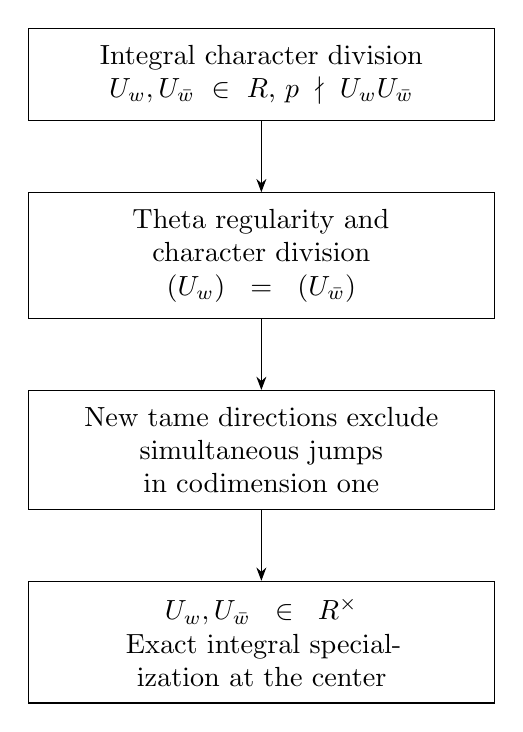
\begin{tikzpicture}[
 box/.style={draw,align=center,text width=5.5cm,inner sep=6pt},
 >=Stealth,node distance=9mm]
 \node[box] (integral) {Integral character division\\
                         $U_w,U_{\bar w}\in R$, $p\nmid U_wU_{\bar w}$};
 \node[box,below=of integral] (theta) {Theta regularity and character division\\
                         $(U_w)=(U_{\bar w})$};
 \node[box,below=of theta] (remove) {New tame directions exclude\\
                         simultaneous jumps in codimension one};
 \node[box,below=of remove] (unit) {$U_w,U_{\bar w}\in R^\times$\\
                         Exact integral specialization at the center};
 \draw[->] (integral)--(theta);
 \draw[->] (theta)--(remove);
 \draw[->] (remove)--(unit);
\end{tikzpicture}
\caption{The pair comparison separates integral divisibility from
divisor removal. The theta implication is used on characteristic-zero
divisors; the final specialization takes place in the integral ring.}
\label{fig:pair-comparison}
\end{figure}

The reusable parts of this argument are the marked residual
obstruction calculation, the integral character-division test, and the
uniform position-cut and product-character estimates. Their roles are
different: the first controls determinant factors above $p$, the
second transfers divisibility from highly ramified characters, and the
third supplies the vanishing implication needed to remove horizontal
factors. We prove the changes needed for these applications rather
than inferring them from the conclusions of the companion papers.

\subsection{Organization}

Section~\ref{sec:classical} fixes the arithmetic inputs and the exact
height and period comparisons. Sections~\ref{sec:models}
and~\ref{sec:vertical} construct the integral diagrams and establish
the residual determinant tests. Section~\ref{sec:single} proves the
single-curve inequality, and Section~\ref{sec:pair} constructs the
integral pair quotients. Sections~\ref{sec:theta}
and~\ref{sec:extraction} prove the theta implication, including the
increasing-level and nonaugmentation estimates.
Section~\ref{sec:unit} removes the quotient divisors.
Section~\ref{sec:center} computes the central arithmetic volume and
completes the proof of Theorem~\ref{thm:main}.

\section{Arithmetic inputs and exact normalizations}\label{sec:classical}

The two comparisons will be carried out at a fixed odd prime. This
section explains the reduction to that problem, constructs the
quadratic fields used in the pair comparison, and records the real
arithmetic identity that converts a Heegner-point index into a sum of
BSD discrepancies. None of these reductions asserts an odd-primary
leading-term equality.

\subsection{The two low-corank inputs}

For a number field $M$, the compact local Kummer condition for the
Tate lattice $T_pE$ is the image of the completed point module
\[
 E(M_v)^{\wedge}_p=\varprojlim_n E(M_v)/p^nE(M_v)
       \longrightarrow H^1(M_v,T_pE).
\]
For discrete coefficients, the local condition is the image of
$E(M_v)\otimes\Q_p/\Z_p$ in $H^1(M_v,E[p^\infty])$. The full Selmer
group uses these conditions at every place. The Kummer exact sequence
is
\begin{equation}\label{eq:kummer-exact}
 0\longrightarrow E(\Q)\otimes\Q_p/\Z_p
 \longrightarrow\Sel_{p^\infty}(E/\Q)
 \longrightarrow\Sha(E/\Q)[p^\infty]\longrightarrow0.
\end{equation}

\begin{theorem}[Unrestricted low-corank converse]\label{classical:low-corank}
For every elliptic curve $A/\Q$, every prime $q$, and $u\in\{0,1\}$,
the equality $s_q(A)=u$ implies
\[
 a(A)=r(A)=u,\qquad \#\Sha(A/\Q)<\infty.
\]
\end{theorem}

This is \cite[Theorem~1.1]{C}. We use its stated conclusion;
we do not interpret its rationalized cohomological construction as
an integral leading-term formula.

\begin{theorem}[Two-primary leading term]\label{classical:two-primary}
For every elliptic curve $A/\Q$ with $s_2(A)\leq1$, the quotient
$Q_A$ of \eqref{eq:normalized-quotient}, with the total real period
and the full-lattice regulator of \eqref{eq:height-convention}, is a
positive rational number, and
\[
 v_2(Q_A)=v_2(\#\Sha(A/\Q)).
\]
\end{theorem}

This is \cite[Theorem~1.1]{B}. Its role here is exactly
the assertion at two, together with positivity and rationality.
After Theorem~\ref{classical:low-corank},
\eqref{eq:kummer-exact} gives $s_p(E)=r(E)$ at every prime. Thus
Theorem~\ref{classical:two-primary} applies to the curve in
Theorem~\ref{thm:main}.

We also use the forward analytic theorem, in order to apply these
conventions to auxiliary twists chosen by analytic nonvanishing.

\begin{theorem}[Analytic rank zero and one]\label{classical:analytic-low-rank}
If an elliptic curve $A/\Q$ has $a(A)\leq1$, then
$r(A)=a(A)$ and the entire group $\Sha(A/\Q)$ is finite.
\end{theorem}

This is the Gross--Zagier--Kolyvagin theorem, using modularity
\cite{GrossZagier,Kolyvagin,BCDT}. By \eqref{eq:kummer-exact} and
Theorem~\ref{classical:two-primary}, $Q_A\in\Q_{>0}$ for every such
$A$. Hence $X_p(A)$ is defined for all the twists used below.
From now on, $p>2$ is fixed, $v=v_p$ on constants, and we abbreviate
$X_p(A)$ to $X(A)$.

\begin{proposition}[Isogeny invariance]\label{classical:isogeny}
Suppose $A$ and $A'$ are isogenous elliptic curves over $\Q$ of
analytic rank at most one. Then
\[
 \frac{Q_A}{\#\Sha(A/\Q)}
       =\frac{Q_{A'}}{\#\Sha(A'/\Q)}.
\]
In particular $X(A)=X(A')$. Over a number field, the corresponding
analytic-to-arithmetic BSD ratio is likewise invariant under isogeny
when the Tate--Shafarevich groups are finite. It is compatible with
products and restriction of scalars.
\end{proposition}

\begin{proof}
These are the arithmetic-volume identities of Cassels and the
restriction-of-scalars comparison of Milne \cite{Cassels,MilneBSD}.
The ratio is formed with the period lattice, full point lattice,
torsion, component factors, and finite Tate--Shafarevich group;
the kernel and cokernel factors of an isogeny cancel in this combined
ratio. The analytic $L$-function is isogeny invariant. Finiteness in
the rational low-rank applications is supplied by
Theorem~\ref{classical:analytic-low-rank}; it passes to the products
and restrictions used here. Thus no conjectural equality of either
ratio with one is required.
\end{proof}

\subsection{Auxiliary quadratic fields}

The pair comparison uses simultaneous nonvanishing for three twists.
We record precisely the density input used for that choice.

\begin{theorem}[Analytic twist densities]\label{classical:twist-density}
For every elliptic curve $A/\Q$, among nonzero squarefree integers
$d$ ordered by $|d|$, the twists $A^d$ of analytic rank zero and one
each have density $1/2$. Consequently the set of $d$ with
$a(A^d)\geq2$ has density zero.
\end{theorem}

We use the theorem at the scope stated in \cite[Theorem~1.2]{Goldfeld}.
Its use below requires no uniform estimate as $A$ varies: one first
chooses one discriminant and then applies the theorem to two fixed
curves. This is the auxiliary-field argument of \cite[Section~2]{C}.

\begin{lemma}[Compatible auxiliary fields]\label{classical:auxiliary-fields}
Let $E/\Q$ have conductor $N$ and analytic rank $r\in\{0,1\}$.
There exist coprime negative odd fundamental discriminants $D,D'<-4$
such that, for
\[
 K=\Q(\sqrt D),\qquad F=\Q(\sqrt{DD'}),\qquad
 L=\Q(\sqrt D,\sqrt{D'}),
\]
the following statements hold.
\begin{enumerate}[label=\textup{(\roman*)}]
\item Every prime dividing $2Np$ splits in both imaginary quadratic
fields, and $\left(\frac{D}{|D'|}\right)=1$.
\item The analytic ranks of $E^D,E^{D'},E^{DD'}$ are respectively
$1-r,1-r,r$.
\item The extension $L/F$ is CM and unramified at every finite place,
and $L$ has only the roots of unity $\{\pm1\}$.
\item One may require $L\cap\Q(E[p])=\Q$ and, when $E$ has CM,
that $L$ not contain its CM field.
\end{enumerate}
Finitely many additional splitting conditions and exclusions of
quadratic fields can be imposed. Both $L(E/K,s)$ and
$L(E^{D'}/K,s)$ have a simple zero at $s=1$.
\end{lemma}

\begin{proof}
Negative odd fundamental discriminants in an admissible fixed
congruence class have positive density. Prescribe splitting at
$2Np$, impose any additional splitting conditions, and exclude a
finite set of quadratic fields. The zero-density exceptional set
in Theorem~\ref{classical:twist-density} cannot exhaust these classes.
We can therefore choose $D$ so that $a(E^D)\leq1$.

Keep $D$ fixed. Choose $D'$ prime to $D$, subject to the same
splitting conditions and, in addition,
$D'\equiv-1\pmod{|D|}$. Together with a sufficiently divisible
modulus supported at $2Np$ and any other prescribed primes, these
conditions contain admissible classes of positive density. Since
$|D'|\equiv1\pmod{|D|}$, quadratic reciprocity gives the required
Jacobi symbol. Apply Theorem~\ref{classical:twist-density} to the
two fixed curves $E$ and $E^D$. The union of their exceptional sets
still has density zero. Thus one can arrange both
$a(E^{D'})\leq1$ and $a(E^{DD'})\leq1$.

For a fundamental discriminant $b$ prime to $N$, the root-number
multiplier is $\chi_b(-N)$. Our splitting and sign prescriptions
make this multiplier $-1$ for $D$ and $D'$, and $+1$ for $DD'$.
The functional equation and the ranks at most one therefore give
the ranks in (ii). The two quadratic factorizations of the
$L$-functions over $K$ prove the last assertion.

The three quadratic subfields of $L$ have discriminants $D,D',DD'$.
The biquadratic discriminant formula yields
\[
 |\operatorname{disc}L|=D^2(D')^2
                       =\operatorname{disc}(F)^2.
\]
The relative discriminant of $L/F$ has norm one, so it is trivial.
The field $F$ is real and $L/F$ is CM. Excluding the finitely many
quadratic subfields responsible for additional roots of unity gives
the last assertion of (iii).

The finite Galois extension $\Q(E[p])/\Q$ has only finitely many
quadratic subfields. A nontrivial intersection with the biquadratic
field $L$ would contain one of the three quadratic subfields of
$L$. Exclude these possibilities when choosing $D$ and $D'$:
after $D$ is fixed, prescribing either $\Q(\sqrt{D'})$ or
$\Q(\sqrt{DD'})$ excludes only finitely many choices of $D'$.
The same argument excludes the CM field. Finite exclusions do not
alter the preceding positive-density argument.
\end{proof}

For the rest of the pair construction, fix such $D,D',K,F,L$ and
write $E'=E^{D'}$ for the companion. In particular $p$ splits
completely in $L$. The rational compact Selmer group over $K$ for
each of $E,E'$ has dimension one. Indeed restriction of scalars is
isogenous to the product of the corresponding two rational twists,
whose analytic ranks sum to one and whose Tate--Shafarevich groups
are finite. A nonzero point in either rank-one line has nonzero
local logarithm at both places above $p$: the kernel of the local
elliptic logarithm on local points is torsion.

\subsection{Heegner points and the height formula}

Put $d_K=|D|$. Let $f\in S_2(\Gamma_0(N))$ be the normalized
rational eigenform attached to $E$. Choose an oriented ideal of
$\mathcal O_K$ of norm $N$ with cyclic quotient, and let $P_X$
be the sum, once over the ideal class group of $K$, of the associated
maximal-order Heegner divisor minus the cusp $\infty$ on $X_0(N)$.
Thus $P_X\in J_0(N)(K)$. There is no division by the class number.

Let $\phi:X_0(N)\to E$ be a rational modular parametrization taking
$\infty$ to zero. We write $\phi_*$ for its map on degree-zero
divisors, and define
\begin{equation}\label{eq:manin-constant}
 P_K=\phi_*P_X,\qquad
 \phi^*\omega_E=c_E f(q)\,\frac{dq}{q},\qquad
 q=e^{2\pi i\tau}.
\end{equation}
The nonzero rational constant $c_E$ is retained exactly; no claim
that it is a $p$-adic unit is used. Write $(f,f)_N$ for the
unnormalized Petersson integral on the ordinary
$\Gamma_0(N)$ quotient, and put
\[
 A_E=\int_{E(\C)}|\omega_E\wedge\overline{\omega_E}|.
\]

Over a number field, $H_{\rm abs}$ denotes the height of
\eqref{eq:height-convention} formed from the absolute logarithmic
$x$-height. It restricts to $H$ over $\Q$. On the Jacobian, use
the Poincare pairing and the orthogonal projector onto the rational
newform factor with its restricted polarization; denote the
resulting absolute diagonal by $H_{\rm abs,f}$.

\begin{theorem}[Split Gross--Zagier normalization]
\label{classical:gross-zagier}
With the preceding conventions, $D$ odd fundamental, $(D,N)=1$,
all level primes split, and $\mathcal O_K^\times=\{\pm1\}$, one has
\begin{align}
 \frac{\sqrt{d_K}}{8\pi^2(f,f)_N}L'(f/K,1)
       &=2H_{\rm abs,f}(P_X),\label{eq:classical-gz}\\
 L'(E/K,1)&=\frac{A_E}{\sqrt{d_K}\,c_E^2}\cdot
                        2H_{\rm abs}(P_K).
                                      \label{eq:classical-gz-elliptic}
\end{align}
In the simple-zero case $P_K$ is nontorsion.
\end{theorem}

The first formula is the conductor-one split Gross--Zagier formula
in the normalization used in \cite[Chapters~I and~V]{GrossZagier};
the conversion is also recorded in \cite[Section~2]{B}. For clarity,
the conversion to the second formula uses the projection formula
for $\phi_*$ and
\[
 (\deg\phi)A_E=8\pi^2c_E^2(f,f)_N.
\]
The relative height over $K$ is $[K:\Q]H_{\rm abs}=2H_{\rm abs}$.
This explains the factor two in both displays. The canonical height
of the origin divisor is $H_{\rm abs}/2$; its Poincare-pairing
diagonal is $H_{\rm abs}$. Thus this convention agrees with
\eqref{eq:height-convention}, without an additional halving.

\subsection{The real arithmetic comparison}

The following equality is needed at odd primes. It is an equality
of real arithmetic ratios before any valuation is taken.

\begin{proposition}[Full-index discrepancy identity]
\label{classical:discrepancy-identity}
Assume $L(E/K,s)$ has a simple zero under the hypotheses of
Theorem~\ref{classical:gross-zagier}. Then
\begin{equation}\label{eq:real-discrepancy}
 \frac{Q_E}{\#\Sha(E/\Q)}
 \frac{Q_{E^D}}{\#\Sha(E^D/\Q)}
 =\frac{[E(K):\Z P_K]^2}
 {c_E^2\prod_\ell c_\ell(E)^2\,\#\Sha(E/K)}.
\end{equation}
The index on the right is the full group index, including torsion.
Consequently, at any prime $p$, if
\[
 n_P=v_p\bigl([E(K)/E(K)_{\rm tors}:\Z\overline P_K]\bigr),
 \qquad \tau_g=v_p(\#E(K)_{\rm tors}),
\]
then
\begin{equation}\label{eq:classical-discrepancy}
 X_p(E)+X_p(E^D)
 =2(n_P+\tau_g)-2v_p(c_E)
             -2\sum_\ell v_p(c_\ell(E))-v_p(\#\Sha(E/K)).
\end{equation}
\end{proposition}

\begin{proof}
Consider $A=\operatorname{Res}_{K/\Q}E_K$. It is isogenous over
$\Q$ to $E\times E^D$. Its point group and Tate--Shafarevich group
are $E(K)$ and $\Sha(E/K)$, and its $L$-function is $L(E/K,s)$.
Its Neron period is $A_E/\sqrt{d_K}$. To see the discriminant
factor, use an integral quadratic basis for $\mathcal O_K$ in the
restriction of the invariant differential; the determinant of the
dual Lie lattice has real Jacobian $1/\sqrt{d_K}$.
The differential stays minimal over $K$: primes of bad reduction
split, and good reduction stays good.

The finite component product for $A$ is
$\prod_\ell c_\ell(E)^2$. At a bad prime, the two split places
each contribute $c_\ell(E)$. At a ramified prime of good reduction,
the special restriction fiber is an extension of the good special
fiber by a vector group and is connected, so there is no extra
component factor. At the remaining good primes the component
factor is one. These period and component calculations are the
restriction-of-scalars arithmetic comparison
\cite{MilneBSD,B}.

Let $P_0$ generate the full free group $E(K)/E(K)_{\rm tors}$,
and write $P_K=mP_0$ modulo torsion. The rank-one regulator for
$A$ is $2H_{\rm abs}(P_0)$; hence
\[
 \frac{2H_{\rm abs}(P_K)}{\Reg_A}=m^2,
 \qquad [E(K):\Z P_K]=|m|\,\#E(K)_{\rm tors}.
\]
Dividing \eqref{eq:classical-gz-elliptic} by the BSD arithmetic
volume just computed gives the right side of
\eqref{eq:real-discrepancy}. Proposition~\ref{classical:isogeny}
identifies the same ratio with the product on its left. Taking
$v_p$ gives \eqref{eq:classical-discrepancy}.
\end{proof}

In \cite[Section~2]{B}, this real identity is subsequently evaluated
at two. The proof above explains why the identity itself applies
at any prime: neither the restriction-of-scalars calculation nor
the Gross--Zagier height identity used a two-primary BSD equality.
What remains in the present paper is to compute the odd-primary
index and Tate--Shafarevich terms on the right of
\eqref{eq:classical-discrepancy} by an exact integral comparison.

\section{Integral cohomology and determinant comparisons}\label{sec:models}

Fix an odd prime $p$.  The arithmetic comparisons below will take place
over power-series rings with coefficients in $\Z_p$, before any
rationalization.  Three features of these comparisons are essential:
specialization is derived, local conditions retain their torsion, and
the duality maps are retained together with the complexes.  We develop
these features first.  The last part of the section records the
specialization criteria that will turn characterwise comparisons into
integral divisibility.

\subsection{Complexes and finite models}

Put $T=T_pE$ and $V=T\otimes_{\Z_p}\Q_p$.  The Weil pairing identifies
$T$ with its Tate dual $T^*(1)$.  Cohomological Frobenius is arithmetic.
Character weights in a theta sum or an Euler factor may therefore use
the inverse of a cohomological character; each such comparison will
specify its convention.  Character corestriction is the unnormalized
sum of translates.  Its restriction to a field killing the character
is the weighted sum with the character giving the required inverse
equivariance, without division by the degree.

For a number field $F$ and a support $S$ containing the places above $p$
and infinity, write
\[
 G(M)=C^\bullet(G_{F,S},M),\qquad L_v(M)=C^\bullet(F_v,M).
\]
Here $M$ is a finite free coefficient module, initially over a finite
local Artin ring.  A local condition is a map $U_v\longrightarrow L_v$.
With $Q_v=\operatorname{cone}(U_v\to L_v)$, its Selmer complex is
\begin{equation}\label{models:selmer-complex}
 C(U,M)=\operatorname{fib}\left(G(M)\longrightarrow\bigoplus_vQ_v\right),
 \qquad \operatorname{fib}=\operatorname{cone}[-1].
\end{equation}
A full condition is the identity and a strict condition is zero.
Global duality uses modified localization at infinity.  Since $p$ is
odd, real Tate complexes are contractible.  The Euler characteristic
of ordinary global cohomology is the negative of the sum of the
negative eigenspace dimensions at real places and the coefficient
ranks at complex places.

The finite-model construction of \cite[Section 3, ``Finite models and
matrix limits'']{B} has the following integral form.  We
give the construction because the residual specialization used in
Section~\ref{sec:vertical} is not a characteristic-zero formal germ.

\begin{lemma}[Finite models and marked operations]\label{models:finite-models}
Consider continuous-cochain diagrams over finite local Artin rings of
$p$-power characteristic, with finite free coefficient modules and
compatible coefficient lifts.  Assume that residual cohomology
dimensions are bounded uniformly, and vanish outside a uniformly
bounded range for every complex for which a bounded model is required.
Then the diagrams admit bounded finite free models with derived base
change.  Restriction, unramified inflation, local cones, cup products,
invariant maps, conjugation, and specified comparison homotopies can be
retained simultaneously.

Suppose the scalar rings at the stages identify with every fixed Artin
precision of a complete local ring $R$ with finite residue field.  On a
fixed nonprincipal ultrafilter $\mathcal U$, the model matrices have compatible
limits over $R$.  Their marked identities survive arbitrary derived
base change, in particular to residue fields of primes of $R$,
including primes containing $p$.  Fixed-group diagrams whose actions
stabilize at every precision compute the actual cohomology of that
group.  A finite diagram may be enlarged on the same stages while
retaining its previous models and markings.
\end{lemma}

\begin{proof}
Continuous cochains with free coefficients over an Artin ring $A$ are
flat: continuous functions are filtered colimits of finite free modules
indexed by finite clopen partitions.  Tensoring them with a finite
scalar module gives the corresponding continuous cochains.  A flat
module over a local Artin ring is free.  Indeed, lift a basis modulo the
maximal ideal; nilpotence proves surjectivity, and flatness followed by
nilpotence proves that the kernel is zero.

Split the residual complex into its cohomology and contractible disks,
and lift the graded bases.  Write $d_0$ for the disk differential and
$i,q,h$ for the inclusion, projection, and contraction, normalized by
$h^2=hi=qh=0$ and $1-iq=d_0h+hd_0$.  For $d=d_0+\epsilon$, the formulas
\begin{equation}\label{models:contraction}
 \begin{aligned}
 I&=(1+h\epsilon)^{-1}i,&Q&=q(1+\epsilon h)^{-1},\\
 H&=h(1+\epsilon h)^{-1},&
 d_{\rm small}&=q\epsilon(1+h\epsilon)^{-1}i
 \end{aligned}
\end{equation}
are finite series in the nilpotent maximal ideal.  Substitution, using
$d^2=0$, gives $dI=Id_{\rm small}$, $Qd=d_{\rm small}Q$, $QI=1$,
and $dH+Hd=1-IQ$.  The remaining ranks are the residual cohomology
dimensions; hence they have the asserted bounds.  Inserting $I,Q$
transfers maps, and inserting $H$ transfers their composition
homotopies.  Tensoring the contractions transfers the cup maps and
their homotopies.  Cones may be formed from transferred maps and then
contracted.

Functions lift across coefficient quotients, so the contractions can
be chosen compatibly.  At a fixed precision the matrices belong to
finite sets.  Their ultrafilter values are therefore defined, and all
finite matrix identities survive passage to the limit.  Exact
triangles survive by retaining their cone identifications; duality
survives by retaining its maps and contracting the comparison cones.
Because the models are free, ordinary tensor of these models is
derived tensor.  No inversion of $p$ enters this argument.

For a fixed group, compare the limiting model at each precision with
a contraction of its actual cochains.  The two compositions are
homotopic to the identities.  These comparisons preserve the marked
maps.  Passing to compact inverse limits introduces no $\lim^1$ term,
by finiteness and compactness.  When the diagram is enlarged, keep the
old contractions, transfer the additional maps, and decrease the
working precision along the ultrafilter if necessary.  Any finite list
of new identities is then retained at a cofinal sequence of precisions.
\end{proof}

The hypotheses hold for the diagrams used here.  The residual
representations belong to a fixed finite list, and the support has
bounded cardinality.  Pass to a fixed finite extension trivializing
these representations and containing $\mu_p$.  Kummer theory bounds
degree one by the fixed unit and class groups and the bounded number
of allowed valuations.  Inflation--restriction, local and global
duality, and the odd-primary cohomological-dimension bounds give the
remaining bounds.  Thus the number of moving primes matters, but
their ramification degrees need not be bounded.

\subsection{Localization and exact orthogonality}

At a non-$p$ place where $M$ is unramified, the unramified complex is
\[
 U_v^{\rm ur}=[M\xrightarrow{\Frob_v-1}M]\quad\text{in degrees }0,1.
\]
Its quotient in the full local complex is residue cohomology on
$M(-1)$, in degrees $1,2$.  Allowing such a place globally while imposing
$U_v^{\rm ur}$ gives the original global complex, by unramified
inflation.  These are the usual localization and purity comparisons;
they hold for the models with their maps, not just for dimensions of
cohomology.

For completeness, the $G_{F,S}$ comparison can be checked after finite
covers trivializing residual coefficients.  In the universal cover,
degree-one classes die as torsors.  Brauer classes die after adjoining
sufficient $p$-power roots of unity, whose local degrees grow at the
finitely many required places, and Picard classes die after
principalization.  Purity, cohomological dimension, and Brauer
reciprocity give higher vanishing.  Real groups have order prime to
$p$.  This proves the comparison on residual coefficients, and the
finite-model construction lifts it to all the coefficients in use.

Locally, first take invariants under the pro-prime-to-$p$ kernel of
inertia, an exact operation, and then use the procyclic tame
$p$-inertia resolution.  A change of generator $z\mapsto z^b$ acts on
its degree-one term by $(z^b-1)/(z-1)$.  If the conjugating powers tend
to $1$ at the retained precisions, both the powers and these geometric
sums tend to $1$.  This observation fixes the local comparison when
the residue cardinalities of moving primes tend to $1$.

After inversion of $p$, at a place with fixed possibly ramified Tate
action and varying unramified scalar, use residue cochains on $V^{I_v}$.
The singular quotient uses $V_{I_v}(-1)$ in degrees $1,2$.  Inertia has
constant linear algebra before the Frobenius scalar is introduced.
These unramified conditions contain all $H^0$ and inject into field
$H^1$.  Their paired cup is nullhomotopic through residue cochains.
On a field fiber their degree-one dimension is $h^0$, and local
duality and Euler characteristic zero identify their exact
complements.

\begin{lemma}[Exact local complements]\label{models:orthogonality}
Let paired perfect local maps $U_v\to L_v$ and $U'_v\to L'_v$ have
a specified nullhomotopy of their cup restriction.  Suppose the
induced morphism
\[
 L'_v/U'_v\longrightarrow U_v^\vee[-2]
\]
is an equivalence, where $\vee$ denotes derived linear dual before
shifting.  Then their Selmer complexes are perfect duals with shift
$-3$.  The localization boundaries for nested such conditions are
adjoint under this duality.  These assertions hold over the model
rings and after localization or derived specialization.
\end{lemma}

\begin{proof}
Let $G_c$ be the compact-support fiber of global localization.
Poitou--Tate pairs $G_c$ with the unrestricted dual global complex
with shift $-3$, and local Tate duality pairs $L_v,L'_v$ with shift
$-2$.  Dualizing $G_c\to C(U)\to\bigoplus_vU_v$ and using the given
local equivalences identifies the dual fiber with $C(U')$.  The same
triangle identifies the boundary maps as adjoints.

At finite precision these are the cup, invariant, and compact trace
diagrams of local and global duality \cite{Milne,Nekovar}.  The top
scalar local and compact cohomology groups, in degrees two and three,
are the coefficient ring; their traces are compatible with reduction
and corestriction.  Retain these maps and the reciprocity homotopy in
Lemma~\ref{models:finite-models}.  Perfectness is checked on the
residue field and lifted by contracting the comparison cone.  This
also proves compatibility after specialization.  For split local
complexes the required nullhomotopies are checked on the split
cohomology; for unramified conditions they are supplied by the residue
factorization above.
\end{proof}

Conjugate transport may identify a coefficient over an imaginary
quadratic field with its Tate dual.  In that convention complements
are imposed at conjugate places.  Under Shapiro, compact and local
invariants are compatible with corestriction; no factor equal to the
quadratic degree is inserted.  Exact orthogonality over the testing
ring is needed throughout.  Orthogonality only after passage to its
fraction field would not suffice for the determinant comparisons.

\subsection{Detection of classes after residual specialization}

The models also allow classes to be tested on sequences of Galois
elements.  This will let Chebotarev produce new primes whose
first-order effects distinguish specified classes.

\begin{lemma}[Evaluation detection]\label{models:evaluations}
Let $G_R(M)$ be an unrestricted limiting global model as in
Lemma~\ref{models:finite-models}.  After any field specialization,
including $R\to\Frac(\F_p[[\mathbf u]])$, its degree-one cohomology
injects into abstract crossed-homomorphism classes on the product of
the stage absolute Galois groups.  The action is obtained by taking
entrywise coefficient limits before specialization.  Invariants are
detected in the same way.  The assertion holds for a Selmer complex
whenever its local conditions contain all local $H^0$ and inject into
local field $H^1$.
\end{lemma}

\begin{proof}
Keep the inclusions of the finite models into actual cochains.  At
residual precision a bounded list of group elements detects
invariants and detects whether the values of a model cocycle have
the form $g a-a$ for one $a$ in the coefficient module.  The bound
comes from linear equations in the coefficient space and in the
bounded model space.  Mark the resulting evaluation map to
$[M\to M^{\rm list}]$ in degrees zero and one.  It is an isomorphism
on residual $H^0$ and injective on residual $H^1$.  Its cone has zero
residual cohomology in degrees at most zero.  A minimal model of the
cone therefore has zero terms there.  This remains true after every
field base change and proves the required injection.

For every sequence of group elements, and every pair or finite tuple
of sequences, the evaluation matrices have compatible limits.
The cocycle and coboundary equations consequently hold on their
product group.  Conjugation identities hold on classes by the marked
homotopies.  The Selmer assertion follows from the localization
sequence and the hypotheses on the local maps.
\end{proof}

Here are two consequences that we will use.  If a normal joint kernel
$J$ acts trivially on the coefficients, restriction gives additive,
equivariant evaluations on $J$.  It detects classes whenever the
quotient has vanishing $H^1$.  A central scalar whose difference from
$1$ is invertible gives this vanishing directly from the crossed
homomorphism identity.  In characteristic zero another useful
quotient test is a normal subgroup consisting of arbitrary sequences
in a fixed deep $\operatorname{SL}_2(\Z_p)$ subgroup, with its standard
plane action and trivial scalar twists.  To see vanishing of even
abstract $H^1$, use a constant diagonal $(m,m^{-1})$, with integer
$m>1$ sufficiently close to $1$, to kill the cocycle on the diagonal.
Conjugation multiplies the upper-unipotent parameter by $m^2$; the
crossed relation and the $m^2$-power formula then kill the upper
unipotent values, since the resulting coefficient matrix is
invertible.  Use the inverse diagonal for lower unipotents, and
Gaussian factorization for arbitrary sequences.  Such a subgroup
remains available in a non-CM Tate image in the presence of competing
data of bounded derived length: sufficiently iterated derived groups
kill those data and still contain a deep special linear subgroup.

For an absolutely simple coefficient representation with scalar
endomorphisms, evaluations of independent detected classes span the
full tuple of coefficient spaces.  Otherwise their equivariant span,
a submodule of a sum of copies of that simple representation, would
give a scalar relation among the classes.  The same holds jointly for
pairwise nonisomorphic simples.  This statement is valid in the
residual fields; it requires neither characteristic-zero
semisimplicity of the Galois group nor an assertion about polynomial
avoidance on a finite field.  We will use its linear span and
bilinearity there.

Finally, a finite table of the evaluations and other continuous
arithmetic data factors through a finite quotient at each retained
precision.  Chebotarev realizes it by a Frobenius representative once
the prescribed splitting conditions are compatible.  Adding primes
uses unramified inflation with its marked homotopies, so evaluations
already made are preserved.  Cup-primitive equations solved in a
field-specialized model are interpreted on these evaluation cochains
using the same inclusions and homotopies.  Reciprocity in this use is
the transferred arithmetic invariant identity, not a reciprocity
assertion for an abstract product group.  Over a fixed finite extension
of $\Q_p$, fixed denominators can be cleared and equations lifted to
increasing precision.  Such clearing is used only after inversion of
$p$.

\subsection{Determinant volumes and switching lemmas}

For a perfect complex define its inverse determinant by
\[
 \mathcal D(C)=\bigotimes_i(\det C^i)^{(-1)^{i+1}}.
\]
At a DVR $A$, let $d(C,y)$ be the valuation of a generic tensor $y$
relative to a generator of this line.  A torsion cohomology group of
length $b$ in degree $i$ contributes $(-1)^{i+1}b$.  In particular, for
a generically acyclic square complex in degrees $1,2$,
\begin{equation}\label{models:determinant-sign}
 d(C,1)=-v(\det d^1).
\end{equation}
Determinants multiply in exact triangles.  Bases and their signs are
understood up to integral units.

The following statements give the precise interfaces of the algebra
lemmas in \cite[Lemmas 3.5 and 3.6]{B}.  Their hypotheses will be verified
at the primes where the switches are used.

Here is the local diagram used in both statements.  At one place
choose conditions
\[
 U_-\subset U_f,U_s\subset U_+,
 \qquad U_f\cap U_s=U_-,\qquad U_f+U_s=U_+,
\]
whose quotients are split free in degree one:
\[
 U_f/U_-=F[-1],\qquad U_s/U_-=S[-1],\qquad
 U_+/U_-=(F\oplus S)[-1].
\]
The conditions contain all local $H^0$; $U_+$ omits local $H^2$.
Write
$C_-,C_f,C_s,C_+$ for the global complexes with these respective
conditions, keeping all other places fixed.  The localization
maps from $H^1(C_f)$ to $F$ and from $H^1(C_s)$ to $S$ are denoted
by $f$ and $s$.  The dual coefficient has the exactly complementary
diagram, and the mixed pairing between the corresponding finite
and transverse quotients is perfect.  A fiber means derived
tensor with the DVR residue field; a generic line has a primitive
fiber reduction by taking a generator of its saturated kernel in
the two-term free model.  The opposite condition in the line
lemma is the complementary condition on the dual coefficient.

\begin{lemma}[Line switch]\label{models:line-switch}
Over a DVR $A$ with residue field $k$, suppose local finite and transverse coordinates are split
free lines in degree one, with perfect mixed pairing.  The lower
condition contains all $H^0$, the upper condition omits $H^2$, and the
global lower and upper diagrams have exact complementary duality.
Assume the finite and transverse global complexes have amplitude
$[1,2]$ on the generic and residual tests.  Suppose the finite complex
has only a generic degree-one line.  At a fiber with
$\dim H^1(C_f\otimes_A k)=h>1$,
assume nonzero finite evaluation both for a primitive reduction of
that line and for some degree-one class of the opposite condition.
Then switching lowers the degree-one dimension by one, and leaves one
generic degree-one line.  If integral classes $Y,Y'$ satisfy
$s(Y')=f(Y)$ under a unit-volume isomorphism of coordinates, then
\[
 d(C_f,Y)=d(C_s,Y').
\]
Successive switches ending at dimension one prove nonnegativity of
this common valuation.
\end{lemma}

\begin{proof}
The generic finite evaluation is nonzero, so the lower complex is
generically acyclic.  In the fiber, reciprocity against the nonzero
opposite finite evaluation prohibits a transverse contribution.
The two localization triangles therefore lower the dimension by one.
Those same triangles identify the class tensors through the common
lower tensor $1$; the local isomorphism changes its volume only by a
unit.  At dimension one the minimal model is a free line in degree
one, and the integral class has nonnegative coordinate valuation.
\end{proof}

\begin{lemma}[Square switch]\label{models:square-switch}
In the preceding local diagram over a DVR $A$ with residue field
$k$, let $F,S$ be split free planes.  Retain all $H^0$ in the lower
condition and omit $H^2$ from the upper condition.  Assume amplitude
$[1,2]$ for both switched global complexes on their generic and
residual tests, exact self-duality of the lower and upper diagrams,
and perfect mixed pairing.  The pure finite and transverse planes
are isotropic, with their compatible cup nullhomotopies retained.
On a common plane let $e$ be unimodular
alternating and $J$ an integral involution, with cross pairing
$e(x,Jy)$ up to a unit.  Suppose the finite complex has generic rank
one in degrees one and two, with class $Y$ and $f(Y)\ne0$, and an
integral transverse class satisfies $s(Y')=Jf(Y)$ up to a unit.  Then
the transverse complex has the same generic ranks and
\[
 d(C_f,(Y,Y^\vee))=d(C_s,(Y',(Y')^\vee)),
\]
where the dual tensor uses the pairing functional on degree two.
If finite evaluation has rank two at a fiber with
$\dim H^1(C_f\otimes_A k)>1$ and is nonzero
on a primitive reduction of $Y$, the switch lowers its degree-one
dimension by two.  Ending at dimension one gives nonnegative
valuation for the class-functional tensor.
\end{lemma}

\begin{proof}
Adjunction identifies the annihilator of the upper localization
image with that same image, so the image is self-annihilating in the
four coordinates.  The two generic classes form a basis of the upper
degree-one space.  In the dual basis of $H^2(C_-)$, write
$Y^*,(Y')^*$ for the functionals normalized to take value one on
their respective upper basis vectors.  These are dual basis
vectors, distinct from the pairing functionals $Y^\vee,(Y')^\vee$
used in the determinant tensors.  Choose a rational complement
$x$ to $f(Y)$ whose boundary is $(Y')^*$.  The cross-pairing gives
$e(x,J s(Y'))$ a unit value, and $s(Y')=Jf(Y)$ therefore makes
$f(Y)\wedge x$ a unit plane volume.  The complement need not be
integral: if both classes are multiplied by a uniformizer
$\varpi$, the normalized dual $(Y')^*$ and this complement
are divided by $\varpi$.
Interchanging the planes gives
the same volume.  Thus both triangles identify the class-functional
tensors with the same lower tensor, proving the equality.  At a
rank-two fiber the upper image is exactly the finite plane, giving
the dimension drop.  At the terminal fiber the model is two free
lines with zero differential and unimodular pairing.  The tensor is
integral there.  Compatible nullhomotopies on the lower comparisons
are part of exact duality and are retained at all unchanged places.
\end{proof}

\begin{lemma}[Strict versus finite conditions]\label{models:strict-finite}
At a split pair $w,\bar w$, let $C_*$ be strict at $w$ and full at
$\bar w$, and let $C_F$ impose exactly complementary finite
conditions $U_w,U_{\bar w}$.  Keep all other conditions fixed with
conjugate duality.  Suppose these comparisons are perfect over a DVR,
$U_w$ is generically a line in degree one, $C_*$ is generically
acyclic, and $Y\in H^1(C_F)$ has nonzero localization.  If
$\operatorname{loc}_wY=a e$ in a generic basis $e$ of $U_w$, then
\begin{equation}\label{models:strict-finite-volume}
 d(C_F,(Y,Y^\vee))=d(C_*,1)+2\bigl(v(a)+d(U_w,e)\bigr).
\end{equation}
Moreover $C_F$ has exactly one generic line in each of degrees one
and two.  Conversely, these line assertions and the nonzero
localization imply the strict acyclicity.
\end{lemma}

\begin{proof}
Use $C_0$, strict at $w$ and finite at $\bar w$, and the triangles
$C_0\to C_F\to U_w$ and $C_0\to C_*\to L_{\bar w}/U_{\bar w}$.
The latter quotient is $U_w^\vee[-2]$.  Its boundary of $e^*$ pairs
with $Y$ by $a$.  The two triangles therefore compare the tensors
with a factor $a^2$, and their local lattice volumes are dual.  This
gives the formula and the rank assertions; the converse follows by
the same nonzero adjoint boundary.  This is the determinant
calculation of \cite[Lemma 3.4]{B}.
\end{proof}

\subsection{The Kummer lattice and its volume}

At an actual scalar specialization the integral local condition is
\[
 U_v^{\rm Kum}=E(F_v)^{\wedge}_p[-1]
 \longrightarrow C^\bullet(F_v,T).
\]
The completed point module includes its torsion.  Its derived
reduction modulo $p^n$ therefore has the invariant $p^n$-torsion in
degree zero and the finite Kummer image in degree one.  The
Bockstein identifies the former with the integral torsion Kummer
classes.  Finite Kummer orthogonality and derived base change show
that these conditions are exact complements.  More explicitly the
cup restriction is null: morphisms from the derived Kummer tensor
to scalars in degree two are detected in top degree, and finite
Kummer pairings vanish for every $n$.  The resulting local quotient
duality is an equivalence on the residue field and hence integrally.

Compact local duality gives
\[
 0\longrightarrow E(F_v)^{\wedge}_p\longrightarrow H^1(F_v,T)
 \longrightarrow
 \Hom(E^\vee(F_v)^{\wedge}_p,\Z_p)\longrightarrow0.
\]
In particular at a non-$p$ finite place the compact degree-one
cohomology is entirely Kummer.  Over $F_v/\Q_p$, the rational
abelian-variety comparison of Bloch--Kato gives
\begin{equation}\label{models:log-exp-pairing}
 \operatorname{inv}_v(z\cup x)
 =\pm\Tr_{F_v/\Q_p}\bigl(\exp^*z\cdot\log x\bigr).
\end{equation}
For $F_v=\Q_p$ and $\exp^*z=\alpha\omega_E$, this is
$\pm\alpha\log_{\omega_E}x$.  This rational comparison includes bad
reduction; it makes no assertion that exponential coordinates are
integral quotient bases \cite{BlochKato}.

\begin{lemma}[Local Haar factors]\label{models:haar}
For the minimal differential, write $P_\ell(1)=L_\ell(E,1)^{-1}$,
$\tau_\ell=\length E(\Q_\ell)[p^\infty]$, and
$\log_{\omega_E}E(\Q_p)=p^l\Z_p$.  Then
\begin{equation}\label{models:haar-identities}
 \tau_\ell=v_p(c_\ell P_\ell(1))\quad(\ell\ne p),\qquad
 \tau_p-l=v_p(c_pP_p(1)).
\end{equation}
The connected real period $\Omega_0$ on a primitive positive Betti
cycle satisfies $\Omega_E/\Omega_0=\#\pi_0(E(\R))$, a $p$-adic unit.
\end{lemma}

\begin{proof}
The measure of the identity-component points for the minimal
differential is the nonsingular residue size divided by $\ell$,
namely $P_\ell(1)$.  Multiplication by the component number gives
$c_\ell P_\ell(1)$.  Away from $p$, the formal subgroup has pro-$\ell$
order and contributes no $p$-primary valuation.  At $p$, a sufficiently
small subgroup is identified by formal logarithm with its additive
lattice.  The $p$-primary part of the logarithm's finite kernel has
size $p^{\tau_p}$, and its image has measure $p^{-l}$; the
prime-to-$p$ kernel contributes a valuation unit.  This gives the
second identity.  The real
identity follows by translation of the minimal differential across
the components.
\end{proof}

\begin{lemma}[Global Kummer volume]\label{models:kummer-volume}
Let $K$ be imaginary quadratic, suppose $E(K)$ has rank one and
$\Sha(E/K)$ is finite, and let $C_{\rm Kum}$ impose the full integral
Kummer conditions.  Put $\tau_g=v_p(\#E(K)_{\rm tors})$ and
$s_K=v_p(\#\Sha(E/K))$.  For a nontorsion point $P$ let $n_P$ be
the valuation of its index in $E(K)/E(K)_{\rm tors}$.  Then
\begin{equation}\label{models:kummer-volume-formula}
 d(C_{\rm Kum},(P,P^\vee))=2n_P+2\tau_g-s_K.
\end{equation}
\end{lemma}

\begin{proof}
Derived Kummer reduction gives the usual finite Selmer groups;
passage to divisible coefficients gives the usual Kummer sequence.
Whole-Sha finiteness therefore identifies integral degree one with
the compact Mordell--Weil module.  The torsion in degree two is the
finite quotient in the compact-to-divisible comparison and has
length $s_K$.  Duality gives torsion length $\tau_g$ in degree three,
as well as a unimodular pairing on the free parts in degrees one and
two.  The torsion lengths in degrees one, two, three are consequently
$\tau_g,s_K,\tau_g$.  Their inverse-determinant contribution is
$2\tau_g-s_K$, and the point and its pairing functional each
contribute $n_P$.  This proves the formula, including under
conjugate-field duality; compare \cite[Section 3, ``Central Kummer
lattices and local measures'']{B}.
\end{proof}

\subsection{Bounded series and specialization}

A bounded series has coefficients in a fixed complete DVR, or in its
fraction field with one common denominator.  This condition excludes
general formal power series over the fraction field.  For measure
coefficients we also use
\[
 \mathcal V=W(\overline{\F}_p),\qquad
 \mathcal V^*=\varprojlim_j\prod_{\mathcal U}(\mathcal V/p^j)
 =W\left(\prod_{\mathcal U}\overline{\F}_p\right).
\]
This is again a complete integer DVR; fixed finite ramification may
be adjoined.  Arithmetic model matrices are first formed over the
smaller rings with finite residual coefficients.  Bounded measures
may then use this larger constant ring.  Fixed character substitution
and fixed finite group quotients commute with the limits.  A tame
cyclic generator is denoted by $1+u$; its relation disappears at every
fixed Artin precision when its $p$-power order tends to infinity.

\begin{lemma}[Division from high characters]\label{models:series-division}
Let $\mathcal O$ be one of these complete integer DVRs and let
$L,B\in\mathcal O[[t,\mathbf u]]$.  Suppose
$L\not\equiv0\pmod{(\varpi,t)}$, where $\varpi$ is a uniformizer.
If, for every sufficiently high finite $p$-power character $\theta$
of $1+t$, the specialization $B(\theta,\mathbf u)$ is divisible by
$L(\theta,\mathbf u)$ after inversion of $p$, then $L$ divides $B$
integrally.  The assertion applies simultaneously to finite products
of such divisors and after the fixed constant extensions above.
\end{lemma}

\begin{proof}
Choose integers $n_j$, one equal to $1$ and the others with suitably
large successive $p$-adic valuations, so that restriction to
$1+u_j=(1+x)^{n_j}$ separates a nonzero leading monomial of the
reduction.  Extend this to a group-power coordinate change.  Then
$L$ is distinguished, up to a unit, in one tame coordinate.
Applying this to a product handles a finite list.  Prescribed
characteristic-zero generic ranks and nonvanishings at $t=0$ may also
be retained: their leading homogeneous forms in logarithmic
coordinates impose finitely many proper conditions on the integer
choices, which can be avoided within the specified congruences.

Divide $B$ by the monic Weierstrass polynomial of $L$.  At each high
$\theta$ its distinguished degree is unchanged, and its quotient
module is $p$-torsion-free.  Thus divisibility after inversion of $p$
makes the integral remainder zero.  Every coefficient of this
remainder, considered as a bounded series in $t$, vanishes at all
high finite characters and is therefore zero by one-variable
Weierstrass preparation.  The argument also applies componentwise
to finite coefficient orders embedded in products of DVRs when the
same residual regularity is retained.  It is the proof of
\cite[Lemma 3.10]{B}, with $p$
in place of two.
\end{proof}

Two further forms of this principle will be useful.  First, a
nonzero bounded one-variable series has, at sufficiently high
characters, valuation equal to its minimum coefficient valuation
plus the first degree attaining that minimum times the valuation
of $\theta-1$.  This is unique dominance; it also proves finite
character avoidance for several variables by iteration.

\begin{lemma}[Persistence of poles]\label{models:poles}
Suppose integral stage numerators and denominators in a genuine
variable converge coefficientwise along the ultrafilter, with
nonzero limiting denominator.  If every stage numerator is
divisible by its denominator after inversion of $p$, each zero
of the limiting denominator in the open unit disk is a zero
of the limiting numerator with at least the same multiplicity.
\end{lemma}

\begin{proof}
Coefficientwise converging integral series converge uniformly on
smaller closed disks.  A zero of multiplicity $m$ of a nonzero
limiting denominator can be isolated on such a disk.  Weierstrass
preparation there retains its zero count on an ultrafilter-large
set.  If stage numerators are divisible by stage denominators after
inversion of $p$, the limiting numerator has at least that
multiplicity.  This pole test permits uncontrolled stage
denominators because boundedness is imposed on numerator and
denominator separately.  Tame characters, when present, are fixed
before this one-variable argument.
\end{proof}

\begin{lemma}[Points on a horizontal divisor]\label{models:field-points}
For a characteristic-zero height-one divisor in a bounded
$\Z_p$-power-series ring, finitely many functions nonzero on that
divisor can be kept nonzero at a point whose coordinates lie in the
open unit disk of a finite extension of $\Q_p$.
\end{lemma}

\begin{proof}
Its prime generator is not divisible by $p$.  A weighted coordinate
change makes it distinguished in one variable.  Modulo its
Weierstrass polynomial the norms of the finitely many nonzero
functions to the remaining power-series ring are nonzero.  Choose
the other coordinates, in finite extensions and in their open
unit disks, avoiding these norms; bounded-series avoidance gives
such a choice.  A root of the distinguished polynomial is also
interior and belongs to a finite extension.  It gives the required
point.
\end{proof}

\begin{remark}[Central determinant coordinates]\label{models:central-pivots}
When the generic and specialized cohomology dimensions agree, a
determinant coordinate specializes using any surviving set of
Gaussian pivots.  One need not keep a particular rational pivot
formula whose denominator vanishes at the point.  At actual central
stage calculations, bounds on torsion lengths and the corresponding
rank tests keep suitable minors nonzero in the limit.  Numerator,
denominator, and class coordinates then converge by their finite
matrix formulas.  This is why retaining torsion in the integral
models is necessary for central valuations.
\end{remark}

\section{Auxiliary primes and residual concentration}\label{sec:vertical}

The characterwise comparisons of the later sections will invert $p$.
They cannot detect a power of $p$ in a determinant.  The purpose of
this section is to choose finitely many tame variables so that the
relevant determinant already has nonzero reduction modulo $p$.
We do this by making first-order deformations separate every
surviving residual Selmer class.  We give both the arithmetic construction
and the residual-field argument, including reducible representations.

\subsection{The two coefficient families}

Use the fields $K,F,L$ and discriminants $D,D'$ of
Section~\ref{sec:classical}.  In particular $p$ splits completely in
$L$, the residual division field is disjoint from $L$, and both
$E/K$ and $E^{D'}/K$ have rank one and finite Tate--Shafarevich group.
There will be two separate tuples of auxiliary primes.  Over $\Q$
the true variable $t$ is the torsion-free cyclotomic variable, and
this comparison is used only for a non-CM curve.  Over $K$ it is the
anticyclotomic variable, with
\[
 \Gamma\simeq\Z_p
\]
the maximal free pro-$p$ quotient of the ring-class tower at $p$.
The order-class exact sequence shows that inertia at either
$p$-place has open image in $\Gamma$.

Fix supports stable under conjugation.  Over $\Q$ include $p$ and
all bad primes.  For $E/K$ include only places over split rational
primes, including both $p$-places and all bad places.  For the
companion also include the primes dividing $D'$.  Any nonsplit place
in this extra support has no inertia invariant, even on residual
composition factors: $E$ has good reduction there, whereas the
quadratic twist is ramified and $p$ is odd.  In each problem over
$K$, include split good prime ideals whose classes generate the
$p$-part of the ideal class group.  Degree-one representatives exist
by Chebotarev.  Additional fixed split good primes may be included;
we may also prescribe exponents at fixed split test primes without
adding them to the cohomological support.  Outside the support the
condition is unramified.

A tame variable $u_j$ comes from a sequence of distinct good primes
$r_{j,i}$, leaving every finite set and tending $p$-adically to $1$.
Over $K$ these primes split completely in $L$.  Its stage character
has cyclic $p$-power order tending to infinity.  Over $\Q$ it is a
conductor-$r_{j,i}$ cyclotomic character.  Over $K$ it is given by a
surjection
\[
 \lambda_{j,i}:\Pic(\mathcal O_{r_{j,i}})\longrightarrow\Z/p^{n_{j,i}}\Z
\]
which is surjective on inertia at each of the two places over
$r_{j,i}$ and satisfies $\lambda_{j,i}^c=-\lambda_{j,i}$.  A chosen
cyclic generator is represented by $1+u_j$.  Rational characters of
$p$-power order are automatically even.

\begin{lemma}[Auxiliary tuples]\label{vertical:auxiliary-tuples}
For any finite list of fixed split support and test primes, the tame
tuple may be chosen to have the following properties.
\begin{enumerate}
\item Its limiting elliptic Frobenius actions have determinant one
and $V(\gamma_j)-1$ invertible.  Over $K$ the same holds for the
companion.  The weight character $\mathcal C$ used in the theta
construction has nontorsion value on each $\gamma_j$, and its
$\Gamma$ value is nonzero.
\item The vectors of Frobenius exponents in the artificial variables
at the prescribed primes are linearly independent over $\Q_p$,
one vector for each rational prime and with one place chosen in
each split pair.  The list includes the coefficient prime $p$.
\item There are at least two moving primes.  Each moving inertia
group maps onto its own cyclic quotient and trivially to the
others.  All fixed conductors and any prescribed finite set of
primes are avoided.
\end{enumerate}
Here $\mathcal C$ is the algebraic anticyclotomic character with
infinity type one and split conductor used in
\cite[Sections 2 and 4]{C}.  Finitely many such fixed characters may
be treated simultaneously.  In the rational case the conditions on
$\mathcal C$ and $\Gamma$ are omitted.
\end{lemma}

\begin{proof}
First prescribe power-residue data.  In the rational case the
radicands are the fixed primes themselves.  In the imaginary case
choose ideal-class generators away from the prescribed places,
generators of their principal power relations, and generators for
expressions of the prescribed prime ideals in those classes.  Include
the conjugates.  For a split prime $\mathfrak q$, take a class-number
power $\mathfrak q^h=(a_{\mathfrak q})$.  The corresponding
anticyclotomic residue exponent is, up to its common generator
normalization, the Kummer exponent of
$a_{\mathfrak q}/\overline{a_{\mathfrak q}}$.  These elements are
independent by their valuations at the chosen split pairs.

Their Kummer image over the cyclotomic tower has full $\Z_p$-rank.
One way to see the required restriction injectivity modulo $p^a$
is to use a central cyclotomic element whose scalar differs from
$1$ by a unit; such an element exists since $p$ is odd and splits
in the fixed fields.  A further fixed finite extension loses at
most a bounded power of $p$.  A $\Z_p$ relation annihilating the
Kummer image would consequently give power relations modulo
arbitrarily high $p$-powers, contradicting the independent
valuations.  Thus sufficiently deep prescribed exponents can be
chosen independently.

To extend an inertia logarithm across the class group, write the
fixed class-group relations in invariant-factor form.  Require the
power-residue exponents to be divisible by the fixed $p$-parts of
these invariant factors, and divide the relations to assign the
values on the ideal generators.  Principal relations then define
the whole character.  Anti-invariance is imposed using the
conjugate generators.  The fixed divisions change neither the full
rational span of the limiting exponents nor their independence.
Finite Chebotarev conditions on roots of unity and on this radical
list realize these power-residue prescriptions.  Taking enough
moving primes gives the independent row vectors in the assertion.

We next check compatibility with the elliptic and fixed character
conditions.  Adjoin all $p$-power roots of elements of the base to
the cyclotomic tower, and consider the joint compact $p$-adic
analytic image of the Tate representation and the fixed characters.
The common Lie quotient with the radical translation group is
abelian.  In the non-CM case it kills the $\mathfrak{sl}_2$ factor
of the Tate image, by Serre's open image theorem \cite{Serre}.
In the CM case, after a fixed extension, the connected Tate image
is a torus.  Conjugation on the remaining abelian analytic quotient
is trivial after a finite extension, whereas conjugation on radical
translations is multiplication by the cyclotomic character.
Choosing that character different from $1$ proves that the common
Lie quotient is zero.  Hence fixing all radicals removes no Lie
dimension from the analytic image.

Make the prescribed radical data sufficiently deep that an identity
neighborhood remains available.  Its determinant-one Tate projection
contains an open special linear subgroup, or an open norm-one CM
torus.  The equation $\det(V(\gamma)-1)=0$ is a proper analytic
condition there.  The weight character is nonconstant by its
nonparallel labelled $p$-adic exponents, and the true
anticyclotomic character is nonconstant by its inertia description.
After shrinking the neighborhood, the torsion condition on the
weight is the zero-logarithm locus.  Avoiding these finitely many
proper analytic loci gives the required Frobenius limits.  The
companion has the same Tate action on $G_L$.

Only finite radical and coefficient tables are used at any stage.
They can therefore be combined into finite Chebotarev prescriptions
with accuracy tending to infinity.  If a bound on
$v_p(r_{j,i}-1)-n_{j,i}$ is required, perturb by a sufficiently high
power of a fixed near-identity element with nontorsion cyclotomic
projection.  Its radical geometric sums vanish to the required
precision, while its cyclotomic displacement has valuation
$n_{j,i}+O(1)$.
No boundedness of the unramified $p$-local degrees of the full
conductor fields is used.
\end{proof}

Put $R=\Z_p[[t,\mathbf u]]$ and let $\chi$ be the product of the
true and artificial character scalars.  Over $\Q$ let $G$ be the
ordinary global complex for $T\chi$, with the moving places allowed.
Over $K$ use the full global complex, also allowing the moving
places, and set
\[
 C_w=\operatorname{fib}(G\longrightarrow L_w^{\rm loc}),
 \qquad w\mid p,
\]
where the condition at the other $p$-place is full.  The residual
restriction kills global $H^0$, and the complementary restriction
at the other $p$-place kills dual $H^0$.  Euler characteristic is
zero.  Thus $C_w$ has a square free model in degrees $1,2$; let
$L_w$ denote its differential determinant, up to a unit.  Use
$L'_w$ for the companion.  Inverting all character conventions
gives the same assertions.

\begin{proposition}[Residual concentration]\label{vertical:tests}
After adjoining finitely many more tame variables, the separate
rational and imaginary tuples satisfy
\begin{equation}\label{eq:source-1}\tag{1}
 \begin{array}{ll}
 \mathrm{(a)}&G\otimes_RR_{(p)}\text{ is a free line in degree one};\\[2pt]
 \mathrm{(b)}&L_w,L'_w\not\equiv0\pmod{(p,t)}
                  \quad\text{for both }w\mid p.
 \end{array}
\end{equation}
\end{proposition}

The proof occupies the rest of the section.  We first describe the
residual cohomology and its parity, then produce a deformation that
kills each residual strict space.

\subsection{Residual spaces and the scalar primitive}

Initially specialize to
\[
 k_r=\Frac(\F_p[[\mathbf u]]),\qquad t=0.
\]
The residual elliptic representation is either absolutely simple or
has character constituents.  Indeed its image contains an element
acting with eigenvalues $1,-1$, even after restriction to $G_K$,
by the disjointness imposed in Section~\ref{sec:classical}.  An
irreducible plane cannot have a quadratic endomorphism field
commuting with this element.  In the reducible case the two
characters are distinct, also over $K$.  Test each simple
constituent, extending the finite coefficient field when necessary,
and include the $\chi$ twist.  Its paired Tate dual has the inverse
twist.

At every finite place in these tests $H^0=H^2=0$.  At fixed split
places the nonconstant Frobenius scalar gives $H^0=0$; at nonsplit
exceptional places inertia does so; at a moving place its own
inertia variable does so.  Apply the same argument to the dual to
obtain $H^2=0$.  Away from $p$, Euler characteristic zero then
makes the full local complex acyclic.  Global invariants vanish
as well.  The strict Selmer degree-one spaces consequently inject
into unrestricted cohomology by Lemma~\ref{models:evaluations}.

Over $\Q$, write $s$ for the dimension of the dual all-strict
space.  Its paired unrestricted primal space has dimension $s+a$,
where $a$ is the negative dimension of the primal constituent at
infinity.  Killing the former space will kill primal $H^2$.
Over $K$, pair the $w$-strict space with the dual $\bar w$-strict
space.  Exact orthogonality and Euler characteristic make their
dimensions equal, say $s$.

\begin{lemma}[Scalar localization]\label{vertical:scalar-localization}
For the constant roots coefficient, global degree-two localization
is injective on these residual tests.  In particular a cup of two
paired classes which is locally zero has a global cochain primitive.
\end{lemma}

\begin{proof}
At residual arithmetic precision, the dual of the localization
kernel is the space of everywhere locally trivial constant
$\F_p$-characters, by Poitou--Tate.  Such a character is unramified
everywhere and split at the support; it is therefore a class-group
character killed by the chosen generating prime classes.  Over
$\Q$ the same group is zero.  The scalar representation and its
cohomological comparison do not depend on the artificial variables.
Tensoring its residual diagram with $\F_p[[\mathbf u]]$ and then
its fraction field preserves this injection.  Equivalently retain
the injectivity cone in Lemma~\ref{models:finite-models}.  Thus a
locally zero degree-two scalar class is zero, giving the primitive.
\end{proof}

\begin{lemma}[Conjugate parity]\label{vertical:parity}
For an absolutely simple residual elliptic plane over $K$, each
one-sided strict space above has even dimension.  The same
alternation statement holds on characteristic-zero localizations
with unramified conditions at fixed non-$p$ places and constant
inertia action.
\end{lemma}

\begin{proof}
Keep $t=0$ and lift the residual test to the $(p)$-DVR of
$\Z_p[[\mathbf u]]$.  Non-$p$ local complexes are contractible
there, since their residual tests are acyclic.  The remaining
one-sided problem is perfect in degrees $1,2$, with conjugate
self-duality.  It is generically acyclic.  To check this last
assertion, specialize centrally in characteristic zero.  The
moving-place singular determinants are nonzero because
$V(\gamma_j)-1$ is invertible.  Inflation therefore gives the
fixed-support problem.  The simple-zero choices give one compact
Selmer line from points, and its localization at either $p$-place
is nonzero because the local logarithm has torsion kernel.  At
non-$p$ places the rational local elliptic cohomology vanishes by
the absence of elliptic invariants, local duality, and Euler
characteristic zero.  The strict--finite triangles of
Lemma~\ref{models:strict-finite} now give strict acyclicity.  A
nonzero central determinant is nonzero generically.

We spell out the sign that controls specialization.  On the induced
coefficient, in its two $K$-coordinates, the pairing is
\begin{equation}\label{vertical:induced-pairing}
 ((a,b),(a',b'))\longmapsto e(a,b')+e(b,a'),
\end{equation}
where $e$ is the elliptic alternating pairing.  This is alternating
and Tate-equivariant, including under complex conjugation, which
swaps the coordinates and reverses $e$.  Its compact cup gives a
graded skew pairing of shift $-3$.  Split-coordinate local
conditions are isotropic.  Unramified conditions have the residue
cup nullhomotopy, and contractible local conditions may be replaced
by zero.  At a newly allowed discriminant place the Tate module is
unramified over $K$; quadratic inertia on the induced coefficient
swaps the two coordinates.  Its invariants form the graph of a
character unit.  Restriction to this graph has the same residue
nullhomotopy, since the residue group has cohomological dimension
one and the quadratic index is invertible.  The real Tate terms
are zero.

Graded cup commutativity, the cone cup, and their homotopies are
identities at finite $p$-power precision.  Transfer them by
Lemma~\ref{models:finite-models}.  Antisymmetrization is allowed
because $2$ is a unit.  On a minimal two-term model the resulting
perfect pairing between degrees one and two identifies the
differential with an alternating matrix: if $P$ denotes the
degree-three pairing, its chain identity gives
$P(x,dy)=P(dx,y)=-P(y,dx)$.  The residual and generic nullities of
an alternating matrix have the same parity.  Generic acyclicity
therefore gives even residual nullity.

This also explains the precise extension of the conjugate
Bockstein argument in \cite[Lemma 12.1 and Corollary 12.2]{B}.
No characteristic-zero division is used in
transferring the pairing to the residual field.  For the later
characteristic-zero localizations the same calculation applies
with the constant-inertia unramified comparisons of
Section~\ref{sec:models}; their nullhomotopies are again the
residue ones.
\end{proof}

\subsection{A new tame direction and its lifting obstruction}

Adjoin a new split tame prime sequence with logarithm $\lambda$.
Require $\lambda$ to vanish at all old places, including the old
moving places, at every stage.  This is achieved by imposing
sufficient radical precision on their ideal relations.  Require
also that the old artificial character on its limiting Frobenius
$\gamma$ have a nonzero exponent.  When the new variable is set
to zero, its local complex is then acyclic over $k_r$; unramified
inflation identifies the enlarged specialization with the old
diagram.

These requirements are compatible with prescribed old evaluations.
Start with an element fixing all radicals from the base and having
the Tate and fixed-character conditions of
Lemma~\ref{vertical:auxiliary-tuples}.  Adjust the old scalar
exponents by old moving-prime inertia.  Such inertia is trivial
on the full Tate module, on the fixed splitting fields and
characters, and on the true anticyclotomic character.  To make
an adjustment fix all radicals too, multiply an inertia element
by its conjugate under an element over the base acting by $-1$
on $\mu_{p^\infty}$.  The radical translations cancel whereas
the old abelian character exponents double.  This factor of two
is invertible.  Existence of the conjugating element follows
from the splitting of $p$ in the fixed fields.  Make these
adjustments term by term, retaining the finite evaluation tables.

\begin{lemma}[Necessary first-order lift test]\label{vertical:lift-test}
Let $x$ be an old strict class and $d$ a class in its paired opposite
space.  Choose a primitive $u$ of their scalar cup,
$du=x\cup d$.  For whole spaces of such classes, fix cochain
representatives on bases, choose the primitives on pairs of basis
elements, and extend these choices bilinearly.  Suppose $x$ lifts
in the new direction, with
derivative satisfying $dx_1=-\lambda\cup x$ in the chosen character
convention.  Put
\[
 A=(M_x(\gamma)-1)^{-1}x(\gamma),
\]
where $M_x$ is the coefficient representation of $x$.  Then the
Frobenius evaluation $z_\gamma$ of $u-A\cup d$ vanishes, up to a
common nonzero sign or coordinate factor.  Over $K$ the necessary
equation is its difference with the conjugate evaluation, since
the conjugate tame logarithm has the opposite sign.  The test is
linear in the new direction and bilinear in $x,d$, and is valid
over $k_r$ as well as over the characteristic-zero field tests.
\end{lemma}

\begin{proof}
The primitive exists by Lemma~\ref{vertical:scalar-localization}.
At each $p$-place one of the paired classes is strict, with the
specified local nullhomotopy; away from $p$ the residual local
complexes are acyclic.  At the later horizontal tests the paired
unramified cups instead vanish through the residue complex of
cohomological dimension one.  Thus the cup is locally zero.
Apply the
arithmetic sum of local invariants to the degree-two cochain
\begin{equation}\label{vertical:primitive-cup}
 x_1\cup d-\lambda\cup u,
\end{equation}
with the simultaneous sign convention making it closed.  At old
places $\lambda$ is zero and the local condition removes the
remaining cup.  At the new place $x,d,u$ are unramified.  The
Frobenius-minus-one operator is invertible, and $A$ trivializes
$x$ in the residue complex.  Subtracting this coboundary leaves
the unramified scalar cochain $u-A\cup d$.  Cup with the tame
direction has invariant equal, up to sign, to its Frobenius value.
Here the Frobenius fixes the $p$-power roots of unity, and the
direction is normalized by the power-residue exponent in the
compatible root basis.  The mixed residue--inertia cup is therefore
the usual local reciprocity pairing.  Over $K$ the two places
give the indicated difference.  If several new directions are
combined, the logarithm of one is unramified at the other new
places and gives no additional mixed contribution.

We verify the residual interpretation explicitly.  Mark the old
global cochain inclusions and their values on the Frobenius
sequences, then use the inflation homotopies in adjoining the
new primes.  Their restrictions to new inertia are zero, and
the induced residue representatives have the Frobenius values
just prescribed.  The invertible residue operator removes their
degree-one cohomology, leaving exactly the scalar residue
cochain above.  Mark its root basis and the mixed cup map too.
All the coboundary corrections, restriction homotopies, and the
compact invariant equation are finite matrix identities from
actual arithmetic diagrams.

To use classes over $k_r$, clear their finitely many denominators
in $\F_p[[\mathbf u]]$, including those in the solution for $u$
and in the inverse residue operator.  The resulting equations
hold in the corresponding localized finite free models.  Any
equation which holds only after that localization becomes an
equation over $\F_p[[\mathbf u]]$ after multiplication by one
more common nonzero parameter denominator.  Now use the Artin
rings $A_b=\F_p[[\mathbf u]]/(\mathbf u)^b$, with the first-order
new variables adjoined as needed.  The prime $p$ is zero
throughout this residual calculation.  The cochain inclusions
and homotopies identify its equations with the corresponding
actual stage arithmetic identities over $A_b$; no lift of an
arbitrary residual solution to $\Z/p^n$ is asserted.  Passing
to the limit in $b$ and then inverting the same
nonzero parameter denominators proves the stated equation over
$k_r$.  This does not divide by $p$.  It also shows that further
field extensions preserve the test.  For characteristic-zero
field points one may instead clear fixed scalar denominators
and increase the arithmetic precision, as in
Lemma~\ref{models:finite-models}.  Thus the primitive computation applies
with its residual arithmetic identities established explicitly.
\end{proof}

\subsection{Spanning the obstruction matrices}

Choose bases $x_1,\ldots,x_s$ of a strict space and
$d_1,\ldots,d_{s+a}$ of the paired opposite space in the rational
case, or $d_1,\ldots,d_s$ in the imaginary case.  For a new
direction use the fixed pairwise primitives $u_{ij}$ with
$du_{ij}=x_i\cup d_j$, extended bilinearly as above.  Its
\emph{necessary lift matrix} at Frobenius $\gamma$
has $(i,j)$-entry $z_\gamma(x_i,d_j)$ from
Lemma~\ref{vertical:lift-test}, or the conjugate difference there
over $K$.  A lifted class with row of coefficients $\alpha$ must
satisfy $\alpha Z_\gamma=0$.  Thus a matrix with zero left kernel
excludes every nonzero lift in that direction.

\begin{lemma}[Obstruction span]\label{vertical:obstruction-span}
For the residual tests above, finitely many new tame directions
have necessary lift matrices whose linear span contains every
$s\times(s+a)$ matrix over $k_r$ in the rational problem, every
$s\times s$ matrix for a reducible constituent in the imaginary
problem, and every alternating $s\times s$ matrix for an
absolutely simple plane in the imaginary problem.  Previously
prescribed Tate actions, radical data, old character actions,
and acyclicity of the new local complexes can all be retained.
\end{lemma}

\begin{proof}
Let $J$ be the termwise joint kernel of the full Tate and old
character actions, including $L$ and the fixed splitting data
over $K$.  It is harmless to retain the fixed character data
as well.  On $J$ the evaluations of $x,d$ are additive.
They detect their classes: old inertia at one moving prime
gives a central element in the quotient image whose scalar
difference from $1$ is invertible.  Apply
Lemma~\ref{models:evaluations}.  Independent classes in a simple
representation have evaluations spanning their full tuple,
jointly for nonisomorphic representations.

In the rational case the opposite representations are already
nonisomorphic on old inertia, which sees $\chi$ and $\chi^{-1}$.
In the imaginary reducible case include the conjugate evaluations.
The resulting four representations are distinct: the elliptic
characters are distinct, and opposite infinite scalar twists
cannot be identified.  For an absolutely simple plane take
$d_j=x_j^c$ under conjugate duality.  The two oppositely twisted
planes are nonisomorphic for the same inertia reason.

Multiply a chosen Frobenius representative by a commutator
$[v,w']$ with $v,w'\in J$.  Since the full Tate action is fixed,
both elements fix the cyclotomic tower.  Their radical actions
are translations in an abelian group.  The commutator therefore
fixes all radicals, as well as the Tate and old character data.
The additive evaluations of $x,d$ on the commutator are zero,
so the local correction involving $A$ is unchanged.  The
primitive equation changes its scalar evaluation by
\begin{equation}\label{vertical:commutator-change}
 -e(x(v),d(w'))+e(x(w'),d(v)),
\end{equation}
up to the fixed sign convention.

Joint spanning and bilinearity now give elementary rectangular
matrices in the rational problem and elementary square matrices
in a character problem.  For a plane over $K$, take the
conjugate difference.  With $d_j=x_j^c$, the transposed
comparison has the opposite sign by Weil skew-symmetry; hence
the changes span $E_{ij}-E_{ji}$, the elementary alternating
matrices.  This uses linear span over $k_r$, not an assertion
that every vector in that span is a single Galois evaluation.
Only finitely many commutators are needed to span the finite
matrix spaces.  Differences from the initial Frobenius test
belong to the span of the resulting directions, so their
linear span has the asserted size.

Realize the required Frobenius representatives by Chebotarev at
increasing finite precision, preserving the radical and
evaluation tables of Lemma~\ref{vertical:lift-test}.  Normalize
all root and tangent bases in the same diagrams.  A common
nonzero sign, or a nonzero scalar multiplying an entire tangent
direction, does not change its span.  For conjugate places use
the transported marking, so the two entries are compared with
the same normalization.
\end{proof}

\begin{proof}[Proof of Proposition~\ref{vertical:tests}]
If a tested strict space is zero no new direction is needed.
Otherwise Lemma~\ref{vertical:obstruction-span} supplies a
linear combination of directions whose necessary lift test has
zero left kernel.  In the plane case this uses
Lemma~\ref{vertical:parity}: $s$ is even and an alternating
matrix with $s/2$ invertible skew blocks is nonsingular.

Work in the enlarged residual ring, localized where the old
variables have fraction field $k_r$ and all new variables are
zero.  The new local complexes are acyclic at this point, so
the specialized global diagrams are the old ones.  Cancel their
unit differential blocks.  In the remaining minimal complex,
the derivative of a lifted degree-one vector in a new tangent
direction is the first-order differential.  A vector in its
kernel would pass every necessary cup test.  The chosen test
has zero kernel, so this first-order differential has full
column rank in that direction.  Some maximal minor of the
actual differential has a nonzero initial term.  It is
therefore nonzero over the enlarged generic residual field,
which kills that strict space.

Take the union of the finite direction lists for all simple
constituents, both sides, and both imaginary curves.  Each test
retains its own slice, since every new local prime was chosen
Frobenius-acyclic there.  Long exact sequences for the residual
composition filtration then give the desired vanishing for
the original representation, including nonsplit extensions.

Over $\Q$ the dual strict vanishing gives $H^2=0$ for the
primal full complex.  Its Euler characteristic is $-1$, so it
has one residual degree-one line.  Minimality first at
$(p,t)$ and then at $(p)$ gives a free line over $R_{(p)}$.
Over $K$, one-sided $H^1$ and $H^2$ vanish at the generic
residual test.  The square determinant consequently has
nonzero reduction modulo $(p,t)$, on both sides and for the
companion.  This is~\eqref{eq:source-1}.
\end{proof}

\subsection{Further directions and characteristic-zero tests}

The same construction will be needed when removing horizontal
divisors.  We record what can be retained, so that the later
commutative algebra need not repeat the arithmetic choices.

Here a \emph{horizontal field test} means the derived fiber over
$k(\mathfrak P)=\Frac(R/\mathfrak P)$ for a height-one prime
$\mathfrak P$ of $R=\Z_p[[t,\mathbf u]]$ with $p\notin\mathfrak P$.
Its local testing ring is the DVR $R_{\mathfrak P}$.  This field
need not be a finite extension of $\Q_p$.  The finite-extension
interior points of Lemma~\ref{models:field-points} are points of
the divisor at which finitely many specified denominators remain
nonzero.  Comparisons then specialize from the localization of
$R/\mathfrak P$ at those denominators, not from its entire
fraction field.  In an enlargement by new variables $\mathbf v$, retaining
an old test means localization at $(\mathfrak P,\mathbf v)$ and
specialization $\mathbf v=0$ before its field fiber is taken.

\begin{lemma}[Preservation under enlargement]\label{vertical:enlargement}
Property~\eqref{eq:source-1}(b) persists when further tame primes
are adjoined, provided each has a nonzero Frobenius exponent
in the preceding artificial variables.  On setting the new
variables to zero, unramified inflation identifies the old
diagram, with the full new-place singular factors retained.
Those factors have nonzero reduction on the residual test.
\end{lemma}

\begin{proof}
At the old residual test the new prime has unramified scalar
Frobenius involving an old variable with nonzero exponent.
Its Frobenius-minus-one determinants are nonzero; the local
complex is acyclic over the residual fraction field.  The
localized full-to-unramified triangle multiplies the
determinant by a nonzero residual singular factor.  Hence
specialization of each enlarged determinant remains nonzero
at the old residual test, which proves the assertion.
\end{proof}

\begin{lemma}[Directions at horizontal tests]\label{vertical:horizontal-directions}
Fix finitely many characteristic-zero height-one field tests
of a tuple satisfying~\eqref{eq:source-1}(b), with at least two
old artificial variables.  One may adjoin finitely many tame
directions, locally zero on all old support, so that the new
prime complexes are acyclic at all these fields and the
necessary lift tests of Lemma~\ref{vertical:lift-test} retain
their commutator-spanning property.  The construction is
compatible with further field extension and with the
primitive unramified conditions at fixed non-$p$ places.
\end{lemma}

\begin{proof}
At a height-one test at least one old inertia scalar has
infinite order: two independent variables cannot both
specialize to roots of unity on a single prime divisor.
Adjust the old Frobenius exponents of a new prime as above.
On a line in an infinite-order coordinate, an elliptic
eigenvalue exception excludes only boundedly many integer
choices.  A sufficiently large finite grid in all the old
exponents therefore avoids the exceptions for the finite
list of fields and both representations.  Keep the
nonzero-exponent requirement, all Tate and fixed character
conditions, and the radical conditions making the new
logarithms zero at old places.  This gives simultaneous
Frobenius acyclicity.

Exact orthogonality at the old unramified places uses
Lemma~\ref{models:orthogonality}.  Their cup contributions
and first-order contributions vanish through its residue
nullhomotopy, since the new logarithm is locally zero.
Scalar localization is obtained from the constant model
and Lemma~\ref{vertical:scalar-localization}; it remains
injective after these characteristic-zero specializations.
The marked cup and primitive proof now gives the lift
identity at each field.  On the joint kernel, evaluations
are detected by the central old inertia scalar, and the
commutator formula~\eqref{vertical:commutator-change}
preserves all the imposed data.  For any finite list of
fields take the union of their direction lists.  Each
retains its own spanning slice; it is unnecessary to
prescribe independent matrices at all fields with a single
prime.  Clearing the finitely many denominators and slowing
precision preserves the comparison identities, also after
field extension.
\end{proof}

The vertical part of the comparison is now fixed integrally.
The later sections may test horizontal divisibility after
inversion of $p$ while retaining the nonzero residual
determinants in~\eqref{eq:source-1}.

\section{The single-curve determinant and its central value}\label{sec:single}

Fix an odd prime \(p\).  In this section \(E/\Q\) is non-CM and has
analytic rank zero or one.  The purpose is to prove
\(X(E)\geq0\), where
\[
 X(E)=v_p(Q_E)-v_p\bigl(\#\Sha(E/\Q)\bigr).
\]
The rank and finiteness conclusions of
Theorem~\ref{classical:analytic-low-rank} are in force.
We first construct an integral element of a power-series
ring.  Its value at the trivial character will be computed separately:
by the dual exponential in rank zero, and by an exact logarithmic
comparison in rank one.  These are different assertions, and both are
needed for the inequality.

We use the inverse determinant and the local-condition conventions of
Section~\ref{sec:models}.  In particular, if a two-term acyclic complex
in degrees \(1,2\) has determinant of differential \(a\), then the
coordinate of its canonical rational trivialization has valuation
\(-v_p(a)\).  This sign will account for the local Euler factors below.

\subsection{Integral Siegel classes and their period coordinate}
\label{single:siegel}

Let \(N\) be the conductor of \(E\) and \(f\) its normalized
newform.  We construct the integral
classes needed for the single-curve comparison and determine their exact
dual-exponential coordinate.  The normalization follows the construction
in \cite[Section~4]{B}; the coefficient prime in that source is two, so
we verify the changes in the construction at an odd prime explicitly.

Let \(E_0\) be the optimal elliptic quotient of \(J_1(N)\), and let
\(C_{\rm cusp}\subset E_0(\overline{\Q})\) be generated by geometric
cusp differences.  Manin--Drinfeld makes this a finite Galois-stable
subgroup.  Replace the curve within its isogeny class by
\(E=E_0/C_{\rm cusp}\); Proposition~\ref{classical:isogeny} preserves
\(X(E)\).  The Abel map, followed by this quotient, gives
\(\pi:(X_1(N),D_N)\longrightarrow(E,O)\), where \(D_N\) is the cusp set;
the map is independent of the base cusp used for the Abel map.
Put \(T=H^1(\overline E,\Z_p)(1)=T_pE\), using the principal pairing,
and \(V=T\otimes\Q_p\).
For \(A=p^k\), \(k\geq0\), put \(L_0=NA\) and let
\(\Pi:(X_1(L_0),D_{L_0})\to(E,O)\) be the \(A\)-degeneracy followed
by \(\pi\).  At the mark \(1/L_0\) the degeneracy is
\(\tau\mapsto A\tau\).  Thus, for a minimal differential \(\omega\),
\[
 \Pi^*\omega=c_FF\,\frac{dq}{q},\qquad
 F(\tau)=Af(A\tau),\qquad q=e^{2\pi i\tau},\quad c_F\in\Q^\times.
\]
Let \(a\) be the primitive generator of
\(H_1(E(\C),\Z)^{G_{\R}}\) oriented by
\(\Omega_0=\int_a\omega>0\).  For \(\xi\in\mathrm{SL}_2(\Z)\),
define \(\delta_\xi\in H^1(E(\C),\Z)\) as the Poincare dual of
\(\Pi_*\xi\{0,\infty\}\), with convention
\(\int_E\omega\wedge\delta_\xi=\int_{\Pi_*\xi\{0,\infty\}}\omega\).

\begin{lemma}[The relative lattice]\label{single:relative-lattice}
Relative pullback and Poincare duality give an integral Galois map
\[
 H^1(\overline{Y_1(L_0)},\Z_p)(1)\longrightarrow T.
\]
For \(A=1\), an integral combination \(\delta=\sum_\xi n_\xi\delta_\xi\)
of finitely many symbols satisfies \(\delta(a)=1\).
\end{lemma}
\begin{proof}
Write \(E_0(\C)=\C/\Lambda_0\).  The connected optimal kernel makes
the map on integral homology onto \(\Lambda_0\).  Quotienting by
\(C_{\rm cusp}\) replaces \(\Lambda_0\) by the lattice generated by it
and lifts of the cusp images.  Relative paths between cusps supply
exactly these additional generators.  Consequently
\(H_1(X_1(N)(\C),D_N;\Z)\to H_1(E(\C),\Z)\) is onto.
The Farey triangulation generates the relative group by the Manin edges
\(\xi\{0,\infty\}\).  The invariant sublattice is saturated, so \(a\)
is primitive; unimodularity of the intersection form now gives the
asserted integral combination.  Pullback by the map of pairs is integral,
and relative Poincare duality gives the displayed etale map.  This is
the Betti and relative-cohomology argument of
\cite[Section~4, ``The integral relative lattice'']{B}, before any choice
of coefficient prime; no Hecke projector is involved.
\end{proof}

We use two level patterns, always with \(v_p(M)\geq6\).
In square order, \(n_1=n_2=M\), \(L_0\mid M\), and the row
\(l=(l_1,l_2)\) is \((0,1)\xi\).
In rectangular order put \(b=N/p^{v_p(N)}\), require
\((b,M)=1\) and \(p^{v_p(L_0)}\mid M\), and take
\[
 n_1=b_1M,\qquad n_2=bM,\qquad l=(Ns,1)=(0,1)\xi,
\]
where \(b_1\mid b\) is a product of complete prime powers dividing \(b\).
The unfilled pattern means \(b_1=1\).
The curve \(Y(n_1,n_2)\) parametrizes elliptic curves with independent
points \(P,Q\) of orders \(n_1,n_2\); independence means that they
embed \(\Z/n_1\oplus\Z/n_2\).  The maps to the marked curve and the
cyclotomic field are specified by
\begin{equation}\label{single:mark-root}
 C=\frac{l_1n_1}{L_0}P+\frac{l_2n_2}{L_0}Q,\qquad
 \eta_M=e_M((n_1/M)P,(n_2/M)Q).
\end{equation}
The coefficients of \(C\) are integers in both patterns; \(C\) has
order \(L_0\), and \(\eta_M\) is primitive of order \(M\).
Fix compatible roots in the algebraic, complex, and \(p\)-adic
realizations, with complex root \(e^{2\pi i/m}\) at order \(m\).

Choose \(c,d>1\) prime to \(6pn_2\), with
\(c,d\equiv1\pmod{L_0}\).  On the universal elliptic curve \(\mathcal E\)
let \({}_c\theta_{\mathcal E}\) be Kato's normalized function of divisor
\(c^2(0)-\mathcal E[c]\), and put
\({}_cg_P=P^*{}_c\theta_{\mathcal E}\), \({}_dg_Q=Q^*{}_d\theta_{\mathcal E}\).
Its norm under \([s]\) is itself if \((s,c)=1\)
\cite[Sections~1--2]{Kato}.
At precision \(p^j\), replace the orders by \(p^jn_1,p^jn_2\), and
let \(P',Q'\) range over their independent division lifts of \(P,Q\).
Take the unnormalized trace of the Kummer cup
\begin{equation}\label{single:K1}
 ({}_cg_{P'})\cup({}_dg_{Q'})\otimes
 e_{p^j}(n_1P',n_2Q')^\vee.
\end{equation}
Here the dual basis sends the displayed primitive root to \(1\), so the
coefficient is \(\Z/p^j(1)\).  Apply the arithmetic edge map, trace
along \eqref{single:mark-root}, and push to \(T/p^j\) by
Lemma~\ref{single:relative-lattice}.  Passage to the inverse limit
defines a class in \(H^1(G_{\Q,S},
T\otimes\Z_p[\Gal(\Q(\mu_M)/\Q)])\), for \(S\) containing the
primes of \(pn_2\) and infinity.
For a finite character \(\nu\) of this Galois group, send the basis
vector at \(\sigma\) to \(\nu(\sigma)\); write \(z_\nu\) for the result
with coefficients in \(T\otimes\Z_p[\nu]\).
All traces, including this character push, are unnormalized.

\begin{proposition}[Integrality and traces]\label{single:siegel-traces}
The classes just constructed are integral away from \(pn_2\infty\)
and compatible with division traces and with corestriction as the
\(p\)-part of \(M\) grows with \(A,c,d,\xi\) fixed.
If \(\ell\nmid cdn_2L_0\) is a fresh prime and is adjoined to both
orders and the root index, the rational norm multiplier is
\begin{equation}\label{single:good-norm}
 1-\frac{a_\ell(f)[\ell]}{\ell}+\frac{[\ell]^2}{\ell},
\end{equation}
where \([\ell]\) sends the determinant root to its \(\ell\)-th power.
For \(q_0^a\parallel b\), \(q_0\nmid b_1\), filling \(q_0^a\)
into the first row gives, at a finite even character \(\nu\),
\begin{equation}\label{single:bad-row}
 z_{\rm filled}=(1-a_{q_0}(f)\nu(q_0)/q_0)z_{\rm before}.
\end{equation}
The trace maps themselves are integral in both assertions.
\end{proposition}
\begin{proof}
Further \(p\)-division gives a Cartesian product of the two lift sets:
independence is automatic since the old tuple is already a basis at
\(p\).  At the old precision the inverse-root twists agree.  Base
change and the projection formula turn the trace of the cup into
the cup of the traces, and distribution recovers the old class.
The mark and lower root also agree when the base \(p\)-level grows.
The functions and their inverses are integral away from the level.
Indeed horizontal valuations follow from their divisors; on a smooth
full-level model every geometric fiber component meets a cusp, where
the Tate leading terms are signs, roots of unity, and powers of
\(1-\zeta\) for nontrivial level roots.  These are units away from
the level.  This also checks quotients of level after pullback.
The relative open curve has lisse geometric cohomology away from this
support, vanishing above degree one.  Its arithmetic edge map lands in
\(H^1(G_{\Q,S},H^1(\overline{Y(n_1,n_2)},\Z/p^j)(1))\).
Edge maps commute with traces and maps of pairs.  Finiteness in degree
zero gives the Mittag--Leffler property needed for compact passage;
the subsequent lattice and coefficient maps are integral.

At \(\ell\), start with the Cartesian division sets, subtract the
tuples whose \(\ell\)-parts lie in a common line \(I\subset\mathcal E[\ell]\),
and add back \(\ell\) times the double-prime-to-\(\ell\) lift.  The zero
pair was subtracted \(\ell+1\) times, which explains this multiplicity.
Distribution on \(\mathcal E/I\) identifies the line sums with the
good Hecke correspondence.  Quotient isogenies raise the Weil roots
to \(\ell\), giving \([\ell]\) and twist scalar \(\ell^{-1}\);
the relative elliptic push has Hecke eigenvalue \(a_\ell(f)\).
This last assertion holds for relative maps because pullback has zero
endpoint-function coordinates and the equality of eigenforms also
holds on path integrals.  The added-back multiplication isogeny raises
the roots to \(\ell^2\); its scalar \(\ell^{-2}\), multiplied by
\(\ell\), gives the last term of \eqref{single:good-norm}.

For row filling, fix \(Q\).  A discarded \(q_0^a\)-division lift of
\(P\) has its \([q_0^{a-1}]\)-image in the order-\(q_0\) line \(I_Q\).
For \(\rho:\mathcal E\to\mathcal E/I_Q\), these lifts are precisely
the preimages under \(\rho[q_0^{a-1}]\) of the prime-to-\(q_0\) point
\(\widetilde P\) satisfying \(\rho^\vee\widetilde P=P\).
Express the other unit by distribution over
\(\rho^\vee\widetilde Q=Q\).  The points \(\widetilde Q\) have order
\(n_2\), and their order-\(q_0\) lines differ from \(\ker\rho^\vee\).
In reverse, the discarded sum is indexed by all lines other than the
line of the source mark, since \(l=(Ns,1)\).  Its branches at mark
\(1/L_0\) are \(\tau\mapsto(\tau+i)/q_0\), \(i\bmod q_0\).
Thus it is \(U_{q_0}\), acting on \(Af(A\tau)\) by \(a_{q_0}(f)\)
because \((A,q_0)=1\).  Root translation and inverse twist contribute
\(\nu(q_0)/q_0\).  This proves \eqref{single:bad-row}, including
\(q_0=2\).  The argument reproduces the geometric correspondences of
\cite[Section~4, ``Good-prime norms and rectangular filling'']{B};
every denominator displayed here is a unit at \(p\).
\end{proof}

We next fix the rational differential coordinate, retaining the absolute
normalization needed for divisibility.  For a nonzero torsion label
\(P=[x\tau+y]\), let \(E_P\) be the algebraic weight-one form
\[
 E_P=-\frac1{2\pi i}\left.
 \sum_{(m,n)\in(x,y)+\Z^2}
 \frac{(\operatorname{Im}\tau)^w}
 {(m\tau+n)|m\tau+n|^{2w}}\right|_{w=0},
\]
where the value is obtained by regular continuation.

\begin{lemma}[Full-level calibration]\label{single:kato-calibration}
In square order, before projection to the elliptic curve, the dual
exponential of \eqref{single:K1} is
\begin{equation}\label{single:full-differential}
 \pm M^{-2}(c^2E_P-cE_{cP})(d^2E_Q-dE_{dQ})\,\frac{dq}{q}.
\end{equation}
The sign is determined by cup, pairing, and orientation conventions
and is common to the determinant components.
\end{lemma}
\begin{proof}
Initially impose \(c,d\equiv1\pmod M\).  Apply
\cite[Theorem~9.5]{Kato} with \(k=2\), \(r=r'=1\), and equal level
orders \(M,M\).  The prime-support containment is automatic, the
range conditions are satisfied, and \(p\mid M\) selects the branch
without an additional Euler operator.  The symmetric power has degree
zero.  Its negative Tate moment is exactly the inverse determinant
\(e_{p^j}(MP',MQ')^\vee\) on the basis coset of division tuples.
The weight-one shifted and Fourier-dual forms agree under the fixed
conventions \cite[Proposition~3.11(1) and Section~4.2]{Kato}.
The theorem therefore gives proportionality to the two brackets in
\eqref{single:full-differential}.  We determine the scalar by residues.

Put \(\Theta(t,q)=(1-t)\prod_{h\geq1}(1-q^ht)(1-q^h/t)\).
The normalized Tate function is
\[
 {}_c\theta(t)=(-1)^{(c-1)/2}q^{(c^2-1)/12}t^{-c(c-1)/2}
                 \frac{\Theta(t,q)^{c^2}}{\Theta(t^c,q)}.
\]
The relation \(\Theta(qt,q)=-t^{-1}\Theta(t,q)\) verifies periodicity
and the divisor; multiplication over \([s]\)-preimages verifies norm
invariance for \((s,c)=1\).  These norms fix the constant uniquely:
the norms under \([2]\) and \([3]\) force its third and eighth powers
to be one.  For \(0<x<1\), \(cx\notin\Z\), put
\[
 J_c(x)=c\lfloor cx\rfloor-\frac{c(c-1)}2
       =c^2B_1(x)-cB_1(\{cx\}),\qquad B_1(x)=x-\tfrac12.
\]
At \(t=q^x\zeta\) the leading coefficient is
\(\pm\zeta^{J_c(x)}\), and the order is
\(xJ_c(x)+(c^2-1)/12-\lfloor cx\rfloor(\lfloor cx\rfloor+1)/2\).
The last two terms are integers, since \((c,6)=1\).

On a determinant component choose the cusp
\(P=q^{1/M}\), \(Q=q^{1/M}\zeta_M^u\), with \((u,M)=1\),
over \(K_0=\Q_p(\mu_M)\).  Set \(M_j=p^jM\) and
\(K_j=K_0(\mu_{M_j})\).  Each pair
\(a_1,a_2\in[0,M_j)\cap(1+M\Z)\) gives a cusp orbit represented by
\(P'=q^{a_1/M_j}\), \(Q'=q^{a_2/M_j}\zeta_{M_j}^u\).
Translation by the old width eliminates the first root index; determinant
primitivity makes cyclotomic Galois act freely on the remaining indices.
There are \(p^{2j}\) such orbits, residue degree \(p^j\), and width
ratio \(M_j/M=p^j\), accounting for \(p^{4j}\) division tuples.
Prime-to-\(p\) roots contribute only fixed data.
With \(x=a_1/M_j\), \(y=a_2/M_j\), the tame symbol has root exponent
\(h\equiv\pm uJ_d(y)a_1J_c(x)\pmod{p^j}\).
All signs have zero Kummer class because \(p\) is odd.  The inverse
twist uses \(\zeta_{p^j}^{\pm a_1u}\), so the twisted residue on
\(G_{K_j}\) is
\(\pm J_c(x)J_d(y)(\chi_{\rm cy}-1)/M_j\pmod{p^j}\).
Abelian transfer and the exponential series give
\[
 \frac{\chi_{\rm cy}^{p^j}-1}{p^jM}
       \equiv\frac{\log\chi_{\rm cy}}M\pmod{p^j}.
\]
Indeed \(\log\chi_{\rm cy}\in p^{v_p(M)}\Z_p\), and every term
of degree at least two has the required valuation.  Residue trace
sums field transfers without a ramification multiplier.  Bernoulli
distribution gives \(\sum_{a_i}J_c(a_i/M_j)=J_c(1/M)\), and likewise
for \(d\); hence the limiting residue is
\(\pm J_c(1/M)J_d(1/M)\log\chi_{\rm cy}/M\).
The dual exponential sends \(\log\chi_{\rm cy}\) to \(\pm1\): pair
with Kummer classes of exponential units and use local reciprocity,
with field trace in the de Rham pairing.  The constant term of \(E_P\)
is \(-B_1(x)\), so the two brackets have nonzero constant terms
\(-J_c(1/M)\), \(-J_d(1/M)\) for the initial choices.  Since
\(dq/q\) has residue \(M\), the scalar is \(\pm M^{-2}\).

For arbitrary permitted smoothings use
\((c_0^2-[c_0]^*){}_c\theta=(c^2-[c]^*){}_{c_0}\theta\).
Changing a row by \(c\) changes its inverse-root basis by \(c^{-1}\),
so the induced differential operator is \(c^2-c\,\mathrm{mult}_c^*\).
Choose \(c_0\equiv1\pmod M\), cancel \(c_0^2-c_0\) rationally,
and repeat on the other row.  This cancellation asserts a rational
identity only; it introduces no claim of integral divisibility.
\end{proof}

\begin{proposition}[The period coordinate]\label{single:period-law}
In square or unfilled rectangular order, for every finite even
character \(\nu\) of conductor dividing \(M\), the coordinate of
\(\exp^*(z_\nu)\) in \(\omega\), in compatible field realizations, is
\begin{equation}\tag{2}\label{eq:source-2}
 \pm\Delta_\nu\frac{L^{(M)}(f,\nu,1)}{\Omega_0}\delta_\xi(a),\qquad
 \Delta_\nu=(c^2-c\nu(c)^{-1})(d^2-d\nu(d)^{-1}).
\end{equation}
The superscript omits all primes dividing \(M\), and the sign is
common across symbols.  In square order with \(A=1\), an integral
combination has \(\delta(a)=1\).  In rectangular order, some choice
of \(A=p^k\) and \(\xi\) with lower row \((Ns,1)\) has
\(\delta_\xi(a)\ne0\).
\end{proposition}
\begin{proof}
Apply the coefficient-prime-independent analytic trace identity of
\cite[Section~4, equation~(K5) and proof of ``The period formula'']{B}
to \eqref{single:full-differential}.  Its inputs are square order,
\(L_0\mid M\), mark \(1/L_0\), even \(\nu\), and
\(c,d\equiv1\pmod{L_0}\), all imposed here.  The two rescaled
weight-one lattice sums cancel \(M^{-2}\).  Row reindexing preserves
the mark and gives \(\Delta_\nu\); Hecke unfolding has indices prime
to \(M\) and gives \(L^{(M)}(f,\nu,1)\).
The relative de Rham push has zero cusp-function coordinates, and its
pairing with \(\overline\omega\) is
\(\pm2i\operatorname{Im}(\int_{\Pi_*\xi\{0,\infty\}}\omega)
\Delta_\nu L^{(M)}(f,\nu,1)\).  Writing
\(\delta_\xi=s_0\omega+\overline{s_0}\overline\omega\) gives
\(s_0+\overline{s_0}=\delta_\xi(a)/\Omega_0\), which proves (2).
These are algebraic differentials and algebraic trace and push maps;
the same identity therefore gives the specified \(p\)-adic coordinate.
Local duality uses field trace, with no character-orbit average.
For rectangular order fill every missing row prime.  Each factor
\(1-a_{q_0}(f)\nu(q_0)/q_0\) is nonzero since \(|a_{q_0}(f)|\leq1\),
and is precisely the additional omitted Euler factor at \(q_0\).
Canceling these factors rationally proves (2) before filling.

The square assertion follows from Lemma~\ref{single:relative-lattice}.
For the rectangular assertion take \(\xi\) with upper row \((1,0)\).
The Fricke relation sends the degenerated path from \(0\) to
\(p^k/(Ns)\) to the path from \(\infty\) to \(-s/p^k\), up to sign.
Rohrlich's theorem in \cite[Theorem~13.5(2)]{Kato}, with prime support
\(\{p\}\), gives a primitive odd character of sufficiently high
\(p\)-power conductor with nonzero central twist.  Odd characters
exist even at \(p=3\), by adjoining a fixed odd tame character to
deep wild characters.  Primitive Gauss--Mellin then makes the weighted
sum of these path integrals nonzero.  If they were all real, complex
conjugation would identify the integrals at \(s\) and \(-s\), and
their sum against an odd character would vanish.  Some imaginary part,
and therefore the corresponding \(\delta_\xi(a)\), is nonzero.
\end{proof}

Finally, rational norm identities can be made integral after one common
nonzero multiplier, uniformly over the abelian fields used here.
By Serre's open-image theorem \cite{Serre}, the commutator image on
\(T\) contains a fixed deep special-linear congruence subgroup.
Its invariants in \(T\otimes\Q_p/\Z_p\) have bounded exponent.
The exact sequence for \(T\subset T\otimes\Q_p\) consequently bounds
the torsion exponent of \(H^1(F,T)\) uniformly for these abelian fields
\(F\).  Multiplying a rationally zero norm error by this bound kills it.

\subsection{The determinant to be made integral}

Let \(S\) contain \(p,\infty\) and every bad prime of \(E\), and fix
the smoothing integers before choosing moving primes.  Their prime
divisors are outside the finite support used for the square classes.
Take the rational auxiliary tuple of Section~\ref{sec:vertical}, with
one tame variable for each moving prime and a genuine cyclotomic
variable \(t\).  Put
\[
 R=\Z_p[[t,u_1,\ldots,u_k]],\qquad M_R=T\otimes_{\Z_p}R(\chi).
\]
Here \(\chi\) takes the chosen generators to \(1+t\) and
\(1+u_j\).  The complex \(G\) is the limiting unrestricted global
complex, with the moving primes allowed in its support.  We retain
the finite-stage complexes with their actual cyclotomic tower, as
well as their reductions modulo every fixed Artin precision.  Let
\(z\in H^1(G)\) be the smoothed square class with symbol evaluation
one and degeneracy \(A=1\).  At each stage choose the square order
\(M\) with prime support exactly \(S_f\) together with the moving
primes, and divisible by the required fixed orders.  Thus its
allowed ramification support and its omitted Euler factors agree.

For a fixed \(q\in S_f\setminus\{p\}\), define
\[
 D_q=\det\left(1-\frac{\chi(\Frob_q)\rho_T(\Frob_q)}q
                         \,\middle|\,V_{I_q}\right).
\]
The subscript denotes inertia coinvariants.  Let \(P_q\) denote the
inverse local \(L\)-polynomial at \(1\), with its unramified scalar
argument in the orientation of the period formula.  The two scalar
arguments may be inverse to one another; at the trivial character
they agree.  The polynomials are respectively quadratic at good
reduction, signed linear at multiplicative reduction, and one at
additive reduction.  Thus they are integral, including when \(p\)
divides a Tamagawa number.  Moreover
\[
 D_q(0)=P_q(0)=L_q(E,1)^{-1}\ne0.
\]
We also use the smoothing series \(\Delta\) of
\eqref{eq:source-2}.  Each of \(D_q,P_q,\Delta\) remains nonzero
modulo \((p,u_1,\ldots,u_k)\): the cyclotomic exponents of the
positive integers \(q,c,d\) are nonzero.  Consequently these factors
have no vertical divisor and are regular in \(t\).

\begin{proposition}[Integral normalized coordinate]\label{single:integral}
The generic cohomology of \(G\) is a line in degree one, and \(z\)
is nonzero on that line.  If \(U_0\in\Frac R\) is its coordinate in
the inverse determinant relative to an integral generator, then
\begin{equation}
 U=\frac{U_0}{\Delta}
       \prod_{q\in S_f\setminus\{p\}}\frac{D_q}{P_q}
       \ \in R\setminus\{0\}.
 \tag{3}\label{eq:source-3}
\end{equation}
\end{proposition}

The argument adapts the horizontal comparisons and division method
of \cite[Section~5, ``Horizontal line switches'' and
``Removal of the fixed divisors'']{B}.  The proof has three parts.
The concentration assertion
\eqref{eq:source-1}(a) treats the divisor \((p)\).  At a
characteristic-zero divisor, auxiliary Euler-system derivatives
compare the coordinate with a coordinate on a free line.  Finally,
rectangular classes remove the divisors of the smoothing and fixed
Euler factors.  The last step is necessary: integrality of the
smoothed class alone does not permit division by \(\Delta\).

\subsection{Horizontal line comparisons}

We use the following three settings.  In the first, the coefficient
ring is the localization of \(R\) at a height-one prime avoiding
\(p\Delta\prod_{q\ne p}D_qP_q\).  In the second, all tame
parameters have been removed and we use the fraction field of the
fixed-support cyclotomic ring.  In the third, at an actual stage,
every tame parameter is specialized to a nontrivial finite
\(p\)-power character \(\eta_j\), while \(t\) is retained.  Write
\(\eta=\prod_j\eta_j\) and
\(\Lambda_\eta=\Z_p[\boldsymbol\eta][[t]]\).  The third setting
uses its generic field or a height-one localization not above \(p\),
and imposes unramified conditions at the old non-\(p\) places.
We require that a fixed Frobenius lift at \(p\), trivial in the
cyclotomic quotient, already kill the dual invariants after twisting
by \(\eta\).  The nonzero exponent vector at \(p\) supplies such
specializations.

\begin{lemma}[Line comparison for a smoothed system]\label{single:line}
In any of these three settings, suppose that the chosen square or
rectangular system class \(z_{\rm sys}\) is generically nonzero.
Then the global complex has a single generic cohomology line in
degree one.  At each of the indicated DVRs,
\begin{equation}
                  d(G_{\rm test},z_{\rm sys})\geq0.
                  \tag{4}\label{eq:source-4}
\end{equation}
In the third setting, \(G_{\rm test}\) denotes the complex with the
unramified old local conditions.
\end{lemma}

\begin{proof}
We verify the local hypotheses before constructing derivatives.
In the first setting, dual local invariants vanish at a fixed
non-\(p\) place by the exclusion of \(D_q\).  At a moving place,
invariance under inertia first forces \(u_j=0\); the remaining
Frobenius equation is nonzero on that divisor because the limiting
Frobenius has determinant one and trace different from two.
At \(p\), choose an inertia element generating the cyclotomic
quotient and a Frobenius lift trivial in that quotient.  The first
invariance equation is regular in \(t\); the second is independent
of \(t\) and nonzero, by the fixed-place exponent condition.  They
have no common height-one component.  In the second setting,
nonconstant cyclotomic action gives the same vanishing.  In the
third, the imposed condition at \(p\) gives it directly.

At an old non-\(p\) place in the third setting, inertia acts through
a constant representation.  The unramified condition is residue
cochains on inertia invariants.  Its quotient is residue cochains
on inertia coinvariants with twist \((-1)\), in degrees \(1,2\).
Its differential has determinant
\[
 D_{q,\eta}=\det\left(1-\frac{\chi_t(\Frob_q)
                     \rho_{V\otimes\eta}(\Frob_q)}q
                         \,\middle|\,(V\otimes\eta)_{I_q}\right).
\]
This is nonzero and equals one at a moving conductor where \(\eta\)
is ramified.  The quotient therefore has zero \(H^1\) over the
DVR itself.  This assertion is made before passing to its residue
field, where the determinant may vanish.  The conditions include
all \(H^0\) and omit \(H^2\).  Unramified cup products factor through
residue cohomology, so are zero; local duality and the Euler
characteristic give exact complementarity, including at the
residue field.  These are precisely the complex conditions needed
by Lemma~\ref{models:line-switch}.

Global invariants vanish by the non-CM open-image argument
\cite{Serre}.  We spell out its use on the limiting diagrams.  In
the product of the stage absolute groups, take the joint kernel of
the Tate action and the abelian and radical data used in the
characters.  The quotient contains arbitrary sequences from a
fixed deep principal subgroup of \(\operatorname{SL}_2(\Z_p)\),
acting trivially on the latter data.  Indeed those data have
bounded derived length, whereas repeated Lie brackets retain
\(\mathfrak{sl}_2\).  The evaluation and diagonal-conjugation
argument of Lemma~\ref{models:evaluations} shows that restriction to
this kernel detects a nonzero degree-one class.  Its evaluations
span the Tate plane by irreducibility.  Both the primal and the
opposite-condition spaces inject into unrestricted global
cohomology, by the local invariant checks above.  Poitou--Tate and
the global Euler characteristic now give amplitude \(1,2\) and
\[
 h=1+h^*,
\]
where \(h,h^*\) are their degree-one dimensions.  This remains
true after any of the line changes below.

Choose a fresh sequence of good primes \(\ell\to1\) in
\(\Z_p^\times\), split to increasing precision on all old scalar
data, whose Tate Frobenius tends to
\[
 \tau=\begin{pmatrix}1&e\\0&1\end{pmatrix},\qquad e\ne0.
\]
The local degree-one cohomology over the testing DVR splits into
the finite line \(T/(\tau-1)T\), measured by Frobenius, and the
singular line \(\ker(\tau-1)\), measured by tame inertia.
The notation here means scalar extension to the testing ring;
\(e\) is a unit there because \(p\) has been inverted.  The
conjugating power in the inertia relation tends to one.  The
finite line is isotropic by inflation, and a pure singular cocycle
has values in the Weil-isotropic invariant line.  The mixed pairing
is perfect.  Taking all \(H^0\), the respective line in \(H^1\),
and no \(H^2\) therefore gives the exact complementary conditions.

A nonzero primal class and a nonzero dual class can both be made
nonzero on the finite line.  On the joint kernel their evaluations
are additive and span the plane.  Each prohibited zero is a proper
affine condition; finitely many such conditions can be avoided in
characteristic zero.  Chebotarev realizes the resulting finite
tables at increasing precision.

The order of the further choices is relevant.  At each stage fix
the cyclotomic base \(K_0=\Q(\mu_M)\) first.  Perturb the desired
unipotent element within the available deep special linear
subgroup so that
\(v_p\det(1-\rho_T(\Frob_\ell))\) is large but finite.  Next
choose \(A_i\) with
\[
 A_i-v_p\det(1-\rho_T(\Frob_\ell))\longrightarrow\infty,
 \qquad \ell\equiv1\pmod{p^{A_i}}.
\]
Require exact splitting in \(K_0\), all earlier derivative fields,
and the \(p^{A_i}\)-th roots of all earlier derivative primes.
These conditions make the new degree-\(p^{A_i}\) conductor-\(\ell\)
field and the earlier derivative fields mutually split at their
conductors.  They are compatible with the finite Tate and
evaluation conditions by the same open-image argument.  A
Frobenius lift trivial in the new derivative field is obtained by
an inertia adjustment.

For a set \(I\) of derivative primes, norm the system class to the
compositum \(K_I\) of their degree-\(p^{A_i}\) fields with \(K_0\),
choose inertia representatives \(\sigma_\ell\) generating their
own cyclic factors and trivial on the other factors, and apply
\[
 D_I^{\rm der}=\prod_{\ell\in I}
                 \sum_{j=1}^{m_\ell-1}j\sigma_\ell^j,
 \qquad m_\ell=p^{A_i}.
\]
The good Euler norm at \(\ell\) is
\[
 p_\ell=\ell^{-1}\det(1-\rho_T(\Frob_\ell)).
\]
There is one fixed nonzero \(p\)-power \(L_*\) which clears all
torsion ambiguities and descent obstructions used in a finite
switching argument.  To see uniformity, the commutator image for
a non-CM curve bounds the exponent of \((V/T)^{G_F}\) over all
abelian fields \(F\) in question.  This bounds \(H^1(T)\)-torsion,
and also the invariants of \(T/p^nT\) that occur in
inflation--restriction.  The obstruction and ambiguity groups
are killed by the same bounded exponent.  The identity
\[
 (\sigma_\ell-1)D_\ell^{\rm der}=m_\ell-N_\ell,
 \qquad N_\ell=\sum_{j=0}^{m_\ell-1}\sigma_\ell^j,
\]
then makes the derivatives invariant modulo \(p^n\), for
\(n\to\infty\) sufficiently slowly.  Descend to \(K_0\), use
unnormalized character corestriction, and pass to the marked
models.  We obtain integral classes \(Z_I\), with
\(Z_\varnothing=L_*z_{\rm sys}\).

Here is the exact local derivative comparison.  Put \(m=m_\ell\).
Let \(b,b_\ell\)
be the lower and upper integral cocycles after all other
derivatives, and put \(F=\rho_T(\Frob_\ell)\).  They vanish on
local inertia: good reduction and the Weil bound exclude the
eigenvalue \(\ell\) in the relevant inertia cohomology.  Put
\(x=b(\Frob_\ell)\), \(x_\ell=b_\ell(\Frob_\ell)\).  The norm
identity gives a coboundary \(dy\) with
\[
 \sum_{j=0}^{m-1}\sigma_\ell^jb_\ell=p_\ell b+dy,
 \qquad (F-1)y=mx_\ell-p_\ell x.
\]
After adjusting the descended cocycle, its restriction is exactly
the derivative of \(b_\ell\).  Its finite value tends to zero
because the derivative coefficient sum is \(m(m-1)/2\).  Applying
\(\sigma_\ell-1\) shows that its singular value is \(-y\), up
to the uniformly bounded loss already cleared.  Finally
\[
 y=m(F-1)^{-1}x_\ell-\ell^{-1}\operatorname{adj}(F-1)x.
\]
The first term tends to zero by the chosen margin on \(A_i\).
A lower coboundary \((F-1)w\) disappears after applying the
adjugate in the limit.  The calculation holds on every translate
before character corestriction.  Therefore
\begin{equation}\label{single:finite-singular}
 f(Z_I)=0,\qquad
 s(Z_I)=\operatorname{adj}(\tau-1)f(Z_{I\setminus\{\ell\}}).
\end{equation}
The map between the two lines is multiplication by \(\pm e\),
and hence is a unit comparison at the testing DVR.  The classes
lift to the complexes with the new conditions; the inclusion of
\(H^0\) and the vanishing of the old singular quotients' \(H^1\)
give the claimed lifts over the DVR itself.

If \(h>1\) generically, choose the two nonzero evaluations above.
Equation~\eqref{single:finite-singular} makes the derived primal
class nonzero on the singular line.  Its pairing with the old
dual class is then nonzero at this prime and zero at all other
places, contradicting reciprocity.  Thus \(h=1\) generically.
At a DVR where the fiber has \(h>1\), use the primitive reduction
of the generic line and a nonzero fiber dual class.  The exact
line-switch Lemma~\ref{models:line-switch} reduces \(h\) by one
and preserves the determinant valuation, because the comparison in
\eqref{single:finite-singular} is a unit.  After finitely many
switches the complex is a free line in degree one and its class
is integral.  The factor \(L_*\) is a unit at this DVR.  Reading
the equalities backwards proves \eqref{eq:source-4}.
\end{proof}

\subsection{Removing the smoothing and Euler divisors}

\begin{proof}[Proof of Proposition~\ref{single:integral}]
At \((p)\), \eqref{eq:source-1}(a) identifies \(G\) with a free
line in degree one.  The class is integral and the normalizing
factors are units there.  This proves nonnegative order at the
vertical divisor once generic nonvanishing is known.

For that nonvanishing, use the second setting in
Lemma~\ref{single:line}.  Rohrlich's finite-support twist
nonvanishing, in the form \cite[Theorem 13.5(2)]{Kato}, applies to
the fixed weight-two newform and characters with conductor
supported at \(p\).  Infinitely many sufficiently ramified even
characters have nonzero central value.  The period formula
\eqref{eq:source-2} therefore makes the fixed-support square class
generically nonzero: a torsion class over the one-variable
power-series ring would vanish at all but finitely many such
characters.  Lemma~\ref{single:line} gives one generic line.
Setting all \(u_j=0\) in the full diagram adds acyclic singular
quotients, since the moving Frobenius limits have
\(\det(1-g_j)\ne0\), where \(g_j\) is the limiting Frobenius
at the \(j\)-th moving prime.  The good norm relations multiply the class
by the nonzero constants \(2-\Tr(g_j)\).  Thus the full diagram
also has a nonzero class on a single generic line.  The first
setting of the lemma now treats every horizontal divisor outside
the fixed factors.

It remains to remove the fixed factors.  Express \(U=g_0/f_0\)
using integral determinant pivot formulas, with \(f_0\ne0\), and
retain integral stage expressions \(g_{0,i},f_{0,i}\).  Specialize
the tame variables to finite nontrivial values
\(u_j=\eta_j-1\), avoiding identically zero denominators and
the prohibited Frobenius values at \(p\).  These specializations
still detect bounded series: repeated one-variable Weierstrass
preparation permits avoidance of any finite collection of
nonzero conditions.  The conditions also hold at sufficiently
precise original stages.

Fix such a stage and a horizontal prime of \(\Lambda_\eta\).
Use a rectangular system with unfilled first row, with
\(b=N_{p'}\), and \(M\) supported only at \(p\) and the active
tame conductors.  Choose a degeneracy \(A=p^k\) and a symbol
with nonzero evaluation.  Smoothing integers \(c',d'\) can be
chosen so that \(\Delta'\) is a unit at this prime.  Indeed
preparation realizes its \(t\)-value as an algebraic point of
the open unit disk.  Use CRT to choose integers tending to one
\(p\)-adically, congruent to one on the required fixed symbol
orders, and with a prescribed nontrivial \(\eta\)-value at one
active conductor and trivial values at the others.  All
coprimalities can be maintained.  At the selected \(t\)-value,
the cyclotomic factor tends to one whereas the chosen constant
weight is nontrivial, so the smoothing factor is eventually
nonzero.  Fix one such choice while applying the line comparison.

Call the resulting class \(z'\).  It has primitive Euler factors
away from \(p\): the only other omitted primes are ramified
conductors of \(\eta\), where the twisted local factor is one.
The same nonvanishing theorem makes \(z'\) generically nonzero.
Lemma~\ref{single:line} gives its integral determinant order with
unramified old conditions.  On changing those conditions to full,
the order changes by
\(-\sum_{q\ne p}v(D_{q,\eta})\).

In the common generic full cohomology line the ratio of the
square and rectangular classes, apart from their nonzero
constant symbol ratio, is
\begin{equation}\label{single:class-ratio}
          \frac{\Delta\prod_{q\in S_f\setminus\{p\}}P_q}
               {\Delta'}.
\end{equation}
To verify the identity rather than merely its character values,
evaluate the two classes at the infinitely many sufficiently
ramified cyclotomic characters with nonzero central value.
Formula~\eqref{eq:source-2} gives exactly the displayed ratio;
omissions at active conductors contribute one.  Clearing the
generic denominators and applying one-variable preparation proves
the identity.  Squaring first gives the same valuation conclusion
if the common orientation sign has not been fixed.  Consequently
the tested quotient \(g_{0,i}/f_{0,i}\) has no horizontal pole,
that is,
\[
 g_{0,i}(t,\boldsymbol\eta-1)/f_{0,i}(t,\boldsymbol\eta-1)
                       \in\Lambda_\eta[1/p].
\]
There is no assertion of a uniform denominator for these stage
quotients.

Every remaining possible pole of \(U\) divides a factor regular
in \(t\).  For such a factor \(H\), take a distinguished
representative and divide the integral numerator by \(H^a\),
where \(a=v_H(f_0)\).  At each permitted finite tame
specialization, the limiting numerator contains all the zeros
of the limiting denominator with their multiplicities.  This
follows from Lemma~\ref{models:poles}: on a smaller closed disk about a zero,
the initially integral numerator and denominator converge
uniformly, and Weierstrass preparation preserves the number of
zeros with multiplicity.  Thus the specialized division
remainder is zero.  Finite-character detection makes the
remainder zero in \(R\).  There are therefore no remaining
height-one poles.  Since \(R\) is factorial, \(U\in R\), proving
the proposition.
\end{proof}

\subsection{A tame height in analytic rank one}

The preceding argument established integrality without identifying
the central coordinate.  In rank one that identification requires
the following exact rational equality.  Return to a fixed support
\(S\), with no moving primes.  Choose its square order to have
prime support exactly \(S_f\).  Let \(z_b\) be the smoothed
class at the trivial character and put
\[
 d_0=\Delta(0)\prod_{q\in S_f}P_q(1),\qquad
 P_q(1)=L_q(E,1)^{-1}.
\]
If the analytic rank is one, \eqref{eq:source-2} makes the
central dual exponential zero.  At non-\(p\) places rational
elliptic cohomology is zero, by local duality and the Euler
characteristic.  Thus \(z_b\) lies in the rational compact
Selmer line.  Finite \(\Sha\) identifies this line with
\(E(\Q)\otimes\Q_p\), so \(\log_\omega z_b\) means its
local elliptic logarithm.  A nontorsion rational point has
nonzero local logarithm, since the kernel on local points is
torsion.

\begin{proposition}[Exact logarithmic comparison]\label{single:logarithm}
If \(\ord_{s=1}L(E,s)=1\) and \(P\in E(\Q)\) is nontorsion,
then
\begin{equation}
 \frac{\log_\omega z_b}{(\log_\omega P)^2}
       =\pm d_0\frac{L'(E,1)}{\Omega_0H(P)}.
       \tag{5}\label{eq:source-5}
\end{equation}
The right-hand quotient is rational, and is interpreted in
\(\Q_p\).  The height is exactly the height \(H\) fixed in the
introduction.
\end{proposition}

Choose \(K_b=\Q(\sqrt{-D})\), with \(-D<-4\) an odd fundamental
discriminant, so that all primes of \(2Np\) and the other fixed
data split, and
\(L(f\otimes\varepsilon,1)\ne0\), where
\(\varepsilon=\varepsilon_{K_b}\).
Lemma~\ref{classical:auxiliary-fields} applies because \(w(E)=-1\).  Choose
an integral polynomial \(\mathcal A\) in Hecke operators away
from \(NDp\) that kills every other level-\(N\) eigensystem and
the Eisenstein types unramified away from \(N\) with conductor
dividing \(N\), including the weight-two trivial pair, while
\(\mathcal A_f\ne0\).
Also choose a good inert prime \(\ell\nmid6NDp\), away from
the Hecke primes occurring in \(\mathcal A\), with
\(a_f(\ell)\ne0\).  Multiplicity one gives the first choice;
open image and Chebotarev give the second.  The finitely many
Hecke coefficient tests have indices \(n\) prime to \(ND\),
with odd \(\ell\)-valuation.

A horizontal sequence consists of primes \(r_i\), integers
\(m_i\to\infty\), and surjections
\[
 \lambda_i:(\Z/r_i\Z)^\times\longrightarrow\Z/p^{m_i}\Z.
\]
The primes \(r_i\) avoid the level, all fixed Hecke primes, and
all the finitely many tested indices.
We require \(r_i\equiv1\pmod{ND}\), \(r_i\to1\) in \(\Z_p\),
and splitting in the Hilbert class field of \(K_b\).  The
characters kill \(p\), the fixed support, smoothing integers,
\(2,3,D\), all tested indices, and the finite model and lift
exceptions introduced below.  Their limiting Tate Frobenius
has determinant one and trace \(a_*\ne\pm2\), with eigenvalues
not roots of unity.  These characters are automatically even
because \(p\) is odd.  Viewed idelically, \(\lambda_i\) has
uniformizer value \(\lambda_i(q)\) at \(q\ne r_i\), negative
residue character at \(r_i\), and zero uniformizer value there.
Over an extension it is composed with the norm.

\begin{lemma}[A nonzero height direction]\label{single:height-direction}
The horizontal sequence can be chosen to define bilinear tame
heights whose rational limits satisfy
\[
 h_\lambda^{K_b}(P_1,P_2)=2h_\lambda^\Q(P_1,P_2)
 \quad(P_1,P_2\in E(\Q)),\qquad
 h_\lambda^\Q(P,P)\ne0.
\]
These heights are compatible with trace in the second argument.
\end{lemma}

\begin{proof}
Let \(G_y\) be the extension of \(E\) by \(\mathbb G_m\) defined
by the Poincare biextension at \(y=\operatorname{pol}(P)\).
Choose a rational lift \(B_P\) of \(P\).  The fiber is a line
torsor, so this lift exists.  Splitting its underlying Tate
modules gives an upper-right Galois block \(\beta(g)g_T\);
\(\beta\) is the Kummer cocycle of \(y\), up to the fixed
polarization sign.  At finite order this follows by identifying
division points of \(y\) with splittings of the extension and
using the Weil pairing to compare two splittings.  Write the
Kummer cocycle of \(B_P\) as \((k,x)\).  Then
\[
                         dk=-\beta\cup x.
\]
Include all ramification and nonintegrality primes of these
data in the finite killed list.

Adjoin to a fixed normal splitting field all cyclotomic
\(p\)-power roots and all \(p\)-power radicals of the killed
primes.  Its relative Galois group has bounded derived length,
so the Tate image over this field still contains a deep
\(\operatorname{SL}_2\).  On the additional Tate kernel the
values of \(x\) span the plane.  Indeed nonzero Kummer classes
remain nonzero over a fixed finite extension; a central
homothety in the open Tate image detects them on its kernel.
The further radical quotient has scalar cyclotomic conjugation,
so cannot support the irreducible Tate plane as a quotient.
Choose an element \(g\) fixing the splitting and radical data,
with determinant-one Tate action of the required trace, and
\begin{equation}\label{single:height-cocycle}
       k(g)-\beta(g)g_T(g_T-1)^{-1}x(g)\ne0.
\end{equation}
For existence, on the joint kernel the commutator of two
elements has \(x=\beta=0\) and \(k\)-value
\(\pm2e(x(h_1),x(h_2))\), where \(e\) denotes the Weil form.
Full span supplies a nonzero value.
Multiplying the chosen \(g\) by such a commutator changes the
left side of \eqref{single:height-cocycle} without changing its
Tate action.  Chebotarev and compatible power-residue bases now
give the asserted \(r_i,\lambda_i\).

We use the biextension construction of \cite[Section~6,
``Tame heights and trace compatibility'']{B}, verifying its
\(p\)-power version here.  Over an extension
containing a ring class field of positive \(r_i\)-power
conductor, the normed character is unramified also above
\(r_i\).  Indeed the split order class sequence identifies the
two residue-unit factors modulo the diagonal and the global
units \(\{\pm1\}\).  For units at one specified split place,
the other component is one.  The local norm subgroup therefore
has residue in \(\{\pm1\}\), which the even character kills.
Sum the local character valuations of a rational
biextension lift relative to its rigidified integral fibers.
Reciprocity gives independence of the lift, and the two
biextension laws give bilinearity.  On a Jacobian this is the
Deligne-pairing intersection formula for disjoint generic
supports, with the common orientation sign.

To define the same height downstairs, note that
\(\#E(\F_{r_i})\to2-a_*\ne0\) \(p\)-adically.  One fixed
\(p^b\) therefore removes every finite \(p\)-primary reduction
part.  After multiplying the first argument by \(p^b\), divide
it by \(p^{m_i}\) in the uniquely \(p\)-divisible local factor.
For lifts \(\mathcal B,\mathcal B'\) before and after division,
apply the local character to
\[
                    \mathcal B/([p^{m_i}]_1\mathcal B').
\]
Changing \(\mathcal B'\) changes this scalar by a
\(p^{m_i}\)-th power.  The two laws give bilinearity; comparison
with integral lifts gives the unramified construction after
extension.  Norming lifts in the second argument proves trace
compatibility.  Passing to limits and dividing by \(p^b\)
defines the stated rational heights.

For the fixed lift \(B_P\), all places except \(r_i\) contribute
zero.  Put \(w_i=(g_{i,T}-1)^{-1}x(g_i)\), with \(p^bw_i\)
integral after enlarging the fixed \(b\).  Correcting division
points by this coboundary leaves the fiber cocycle
\(p^b(k-\beta\cup w_i)\).  Its Frobenius value is the power
residue character of the scalar ratio above.  Thus the limiting
height is, up to sign, \eqref{single:height-cocycle}, and is
nonzero.  Trace over \(K_b/\Q\) contributes its degree two.
\end{proof}

Use the square classes with the additional prime \(r_i\), and
write \(\chi_b=(1+u)^{\lambda_i}\).  Since \(\lambda_i(p)=0\),
the local coefficients at \(p\) are split.  Let \(Z_i(u)\) be
the group polynomial of dual-exponential coordinates in
\(\omega\).  Local splitting makes every group coefficient
pass through the same fixed map
\(\exp^*:H^1(\Q_p,T)\to\Q_p\omega\).  Its image has a
fixed denominator lattice, so the denominators of \(Z_i\)
are bounded independently of \(i\).  Moreover \(Z_i(0)=0\).
For nontrivial characters,
\[
              Z_i=\pm d_0 L(f,\overline{\chi_b},1)/\Omega_0.
\]
All these characters are primitive at \(r_i\); there is no
omitted \(r_i\)-factor in this formula.  Write \(Z'\) for the
linear coefficient of the bounded-series limit.

\begin{lemma}[Cup comparison]\label{single:cup}
For the sequence of Lemma~\ref{single:height-direction},
\begin{equation}
 Z'\log_\omega P
  =\pm(2-a_*)\frac{\log_\omega z_b}{\log_\omega P}
                        h_\lambda^\Q(P,P).
 \tag{6}\label{eq:source-6}
\end{equation}
\end{lemma}

\begin{proof}
At stage \(i\), write a cocycle modulo \((p^{m_i},u^2)\) as
\(z_0+uz_1\).  Then \(dz_1=-\lambda_i\cup z_0\).
The good norm relation and one fixed clearing factor permit
the adjustment
\[
 z_0=\alpha_i\beta,\qquad
 \alpha_i=\pm\left(1-\frac{a_f(r_i)}{r_i}+\frac1{r_i}\right)
                              \frac{\log_\omega z_b}{\log_\omega P}.
\]
The clearing is uniform because the degree-one torsion has
bounded exponent.  The scalar two-cocycle
\(z_1\cup x+\alpha_i\lambda_i\cup k\) is closed.  Its local
invariant at \(p\) tends to \(Z'\log_\omega P\), by the
logarithm--dual-exponential pairing.  At the other fixed places
the character is killed and the rational local class is a
coboundary.  At \(r_i\), use \(dw_i=x\) to obtain
\(\alpha_i\lambda_i\cup(k-\beta\cup w_i)\).  Its invariant is
\(\pm\alpha_i h_i^\Q(P,P)\), by the scalar-ratio computation
in Lemma~\ref{single:height-direction}.  The sum of local
invariants is zero.  Passing to the limit, the Euler factor
tends to \(2-a_*\), giving \eqref{eq:source-6}.
\end{proof}

\subsection{The exact spectral comparison}

Fix a rational modular parametrization \(\phi:X_0(N)\to E\),
of degree \(\delta_\phi\).  Let \(P_X\in J_0(N)(K_b)\) be the
single oriented Hilbert-class trace based at \(\infty\), and
put \(Q_X=\phi_*P_X\).  With unnormalized Petersson integral set
\[
                        C_0=\frac{\sqrt D}{8\pi^2(f,f)_N}.
\]
Choose a real primitive period \(\Omega_{\rm tw}\) for the
negative twist.  The period relations are
\[
 C_0\Omega_0\Omega_{\rm tw}\in\Q^\times,
 \qquad L(f\otimes\varepsilon,1)/\Omega_{\rm tw}\in\Q^\times.
\]
The second is modular-symbol rationality.  For the first, if
\(\phi^*\omega=c_\phi f\,dq/q\), the complex area of \(E\)
is \(8\pi^2c_\phi^2(f,f)_N/\delta_\phi\); the twist period is a
rational multiple of the anti-invariant period divided by
\(\sqrt D\).  This also specifies the rational normalization
in which the following identities are embedded in \(\Q_p\).

\begin{lemma}[Spectral-height identity]\label{single:spectral}
For the horizontal sequence just constructed,
\begin{equation}
 C_0\Omega_0L(f\otimes\varepsilon,1)\frac{Z'}{d_0}
       =\pm(2-a_*)\frac{h_\lambda^{K_b}(Q_X,Q_X)}{\delta_\phi}.
       \tag{7}\label{eq:source-7}
\end{equation}
\end{lemma}

\begin{proof}
The proof evaluates the same finite differences of kernel
coefficients in two ways.  Projection onto the \(f\)-block
expresses them through \(Z'\); their intersection interpretation
expresses them through \(h_\lambda^{K_b}(Q_X,Q_X)\).  Matching
the two evaluations, with their constants, gives the identity.
We first specify the finite-character formulas and then prove
their interpolation in the present \(p\)-power direction.
They are the complex coefficient and geometric intersection
identities in \cite[Section 6, ``The traced coefficient,''
``Fricke transformation and unfolding,'' and
``Intersection realization'']{B}.
Their hypotheses are an odd fundamental discriminant \(-D<-4\),
split Heegner level \(N\), a prime \(r\nmid ND\) split in the
Hilbert class field with \(r\equiv1\pmod{ND}\), an even
prime-conductor character \(\chi\) with \(\chi^2\ne1\), and
indices \(nr^h\) with \((n,ND)=1\) and odd valuation at the
chosen inert prime \(\ell\).  None of these identities has a
coefficient-prime hypothesis.

Here are their precise normalizations.  Choose integral ideal
representatives \(C\) of \(\Pic(\mathcal O_{K_b})\), prime to
\(D\), and put \(a_C=\mathrm NC\).
Let \(e(x)=\exp(2\pi i x)\) and
\[
 \theta(z)=\frac12\sum_C\sum_{x\in C}e(\mathrm Nx\,z/a_C).
\]
Its positive coefficient is
\(\rho(n)=\sum_{d\mid n}\varepsilon(d)\).  If \(\theta_\chi\)
is its Fourier twist, define
\[
 E_{\chi,s}(z)=\frac12
  \sum_{\substack{(c_1,d_1)\ne(0,0)\\ND\mid c_1}}
    \varepsilon(d_1)\bar\chi^2(c_1)
       \frac{\operatorname{Im}(z)^s}
            {(c_1z+d_1)|c_1z+d_1|^{2s}},
 \qquad
 I_\chi=\left.\frac{\sqrt D}{2\pi}
    \Tr_{NDr^2/Nr^2}(\theta_\chi E_{\chi,s})\right|_{s=0}.
\]
Characters are extended by zero at nonunits; the trace is
unnormalized.  The continuation is holomorphic.  Poisson
summation pairs the odd row weights, eliminates the
nonholomorphic modes, and permits pairing with cusp tests.

For every tested index \(n\) and \(h\ge1\), regard the
coefficient at \(nr_i^h\) as a polynomial
\(D_{i,h}(n;u)\) in
\(\Z_p[u]/((1+u)^{p^{m_i}}-1)\): in the following sum
\(r=r_i\) and \(\chi(x)=(1+u)^{\lambda_i(x)}\).
\begin{equation}\label{single:kernel-coefficient}
 D_{i,h}(n;u)=\frac12
 \sum_{\substack{C,\ y\in C,\ b>0\\
       a=\mathrm Ny/a_C>0\\ a+Nb=nr^hD}}
 \sum_{\substack{kl=b\\\gcd(k,l,D)=1}}
 W(k)\chi(a/D)\bar\chi^2(Nk),
\end{equation}
where
\[
 W(k)=\prod_{\substack{q\mid D\\q\mid k}}(l/q)
            \prod_{\substack{q\mid D\\q\nmid k}}(-a_CNk/q).
\]
Write \(\epsilon_q(x)=(x/q)\).  The local partial Fourier
transform at \(q\mid D\) has scalar
\(\kappa_q=q^{-1}\tau_q\epsilon_q(-a_CD/q)\), with
\(\tau_q=\sum_{x\bmod q}\epsilon_q(x)e(x/q)\).
Multiplying the partial traces
and the Poisson factor \(-2\pi i/D\) leaves common scalar one,
because the primitive Gauss sum of \(\varepsilon\) is
\(i\sqrt D\).  This explains in particular the factor \(1/2\)
in \eqref{single:kernel-coefficient}.  For a trace matrix
\(\gamma=\left(\begin{smallmatrix}a_\gamma&b_\gamma\\
c_\gamma&d_\gamma\end{smallmatrix}\right)\in\Gamma_0(Nr^2)\),
translation of the theta twist multiplies its weight by
\(\chi(a_\gamma^{-2})\), canceled by the Eisenstein row
weight \(\chi^2(a_\gamma)\).  Thus these
finite-character computations apply to our characters as soon
as \(\chi^2\ne1\), which holds for every nontrivial
\(p\)-power character.

Use the same marked Artin limits as before to define
\(D_h(n;u)=\lim_i D_{i,h}(n;u)\) and
\(D'_h(n)=[u]D_h(n;u)\).  Only terms with \(a\) a unit at
\(r\) occur in \eqref{single:kernel-coefficient}.  Since
\(r\mid nr^h\), this is equivalent to \(k,l\) being units
there.  The identity \(W(l)=-W(k)\) cancels the
divisor-independent terms in the derivative of the character
weight.  Hence \(D'_h(n)\) is the limit of the masked sum
with weight \(-2\lambda_i(k)\).

For \(h\ge0\), define \(B_{i,h}(n)\in\Z/p^{m_i}\Z\) by
the same sum with the mask removed and character weight
replaced by \(-2\lambda_i(k/r_i^{v_{r_i}(k)})\).  Write
\(B_h(n)\) for its Artin limit, put \(B_h(n)=0\) for
\(h<0\), and set \(C_h(n)=B_h(n)-B_{h-2}(n)\).
Stripping a common power \(r^j\) from \(a,b\) shows that,
for \(h\ge2\),
\begin{equation}\label{single:mask}
 C_{h+1}-2C_h+C_{h-1}=D'_{h+1}+2D'_h+D'_{h-1}.
\end{equation}
For completeness, when the primitive index is positive the
\(C_h\)-multiplicities are \(1,4,8,12,\ldots\); their second
differences are \(1,2,1\).  At primitive index zero they are
affine and the second difference is zero.  The off-\(r\)
weights do not change, since the primes over \(r\) are principal
and \(r\equiv1\pmod D\).  This proves the identity for
\(\Z/p^{m_i}\)-valued weights and then on their limits, with
no alteration of constants.

The symbols \(D'_h,B_h,C_h\) will also denote these coefficient
functions of \(n\).  The Hecke polynomial \(\mathcal A\)
acts on them by the weight-two coefficient rule
\((T_s a)(n)=a(sn)+s a(n/s)\), with the second term zero
unless \(s\mid n\).  All its primes are away from \(NDr_i\).
The finite set of tested indices was chosen to contain the
indices needed to evaluate this polynomial at \(n=\ell\).

We next project its holomorphic side.  At level \(Nr^2\) use
\(f_j=r^jf(r^jz)\), \(0\le j\le2\), and write
\(\tau(\chi)=\sum_{x\bmod r}\chi(x)e(x/r)\).
The finite-character Fricke and unfolding identities are
\begin{equation}\label{single:old-pairings}
 \frac{(I_\chi,f_2)_{Nr^2}}{(f,f)_{Nr^2}}
     =\frac{C_0}{r+1}\frac{\tau(\chi)}{\tau(\bar\chi)}
                L(f,\bar\chi,1)L(f\otimes\varepsilon,\bar\chi,1),
 \qquad (I_\chi,f_1)_{Nr^2}=0.
\end{equation}
The exact constants arise from the kernel factor
\(\sqrt D/(2\pi)\), the Fricke factor \(r\), the Mellin integral
\(1/(4\pi)\), and the level index \(r(r+1)\).
At primes of \(N\), use the primitive degree-at-most-one
polynomial and \(\varepsilon(q)=1\); at primes of \(D\) the
twisted local factor is one; at \(r\) both twisted factors
are one.  The total nebentypus is trivial.  The conductor-\(r\)
new cuspidal block is therefore Steinberg, with \(U_r=\pm1\),
and its complementary raises have eigenvalue zero.  The
conductor-\(r^2\) cuspidal block has \(U_r=0\).  In a
ramified Eisenstein pair both characters are ramified at \(r\),
so its \(U_r\)-eigenvalue is also zero.
Thus \(U_r^h(U_r^2-1)\) kills these blocks for sufficiently
large \(h\).  The remaining old blocks come from level \(N\);
the fixed operator \(\mathcal A\) kills all of them except
the \(f\)-block.

Write \(a_h=a_f(r^h)\) and \(a=a_f(r)\).  The normalized
Gram matrix of \(f_0,f_1,f_2\) has entries \(g_{|i-j|}\), where
\[
 g_0=1,\qquad g_1=\frac a{r+1},\qquad rg_2=ag_1-1.
\]
The coefficient vector at index \(nr^h\), after removing its
\(n\)-factor, is \((a_h,ra_{h-1},r^2a_{h-2})\).  The
coefficient of the Gram row for \(f_2\) is
\[
 s_h=\frac{r^2a_{h-2}-g_1ra_{h-1}}{1-g_1^2}.
\]
Its denominators have bounded \(p\)-valuation because
\(a_*\ne\pm2\).  Set
\(\gamma_h=\lim_i(a_f(r_i^h)-a_f(r_i^{h-2}))\).  The
Hecke recurrence gives
\[
 \lim_i\frac{s_h}{r_i+1}
       =\frac{\gamma_h}{(a_*-2)(a_*+2)}.
\]

All factors in \eqref{single:old-pairings} have bounded group
polynomial realizations.  The Gauss ratio is
\(\tau(\chi)^2/r\); its coefficients are integral and fixed
by \(p\)-Frobenius because \(\lambda_i(p)=0\), and its
limiting augmentation is one.  The first \(L\)-value factor
is \(Z_i/d_0\).  For the companion, use the even additive
modular-symbol sum multiplied by \(\tau(\bar\chi)/r\).
Its denominators are bounded by the fixed relative period
lattices.  Before Gauss multiplication its augmentation is
\[
 r\sum_{r\mid j}\frac{a_{f\otimes\varepsilon}(j)}j
    -L(f\otimes\varepsilon,1)
      =(a_f(r)-2)L(f\otimes\varepsilon,1),
\]
by the Hecke recurrence and Mellin continuation.  The trivial
Gauss sum is \(-1\), so its limiting normalized augmentation
is \((2-a_*)L(f\otimes\varepsilon,1)/\Omega_{\rm tw}\).
Multiply the finite-character identity by \((1+u)^2-1\) to
remove the excluded character values, pass to bounded-series
limits, and cancel the nonzero multiplier.  Since \(Z_i(0)=0\),
only that companion augmentation contributes to the derivative.
We obtain
\begin{equation}\label{single:projected-derivative}
 \begin{split}
 [\mathcal A(D'_{h+2}-D'_h)](\ell)
   ={}&\pm\mathcal A_fa_f(\ell)
       \frac{\gamma_{h+2}-\gamma_h}{(a_*-2)(a_*+2)}\\
      &\hspace{4mm}\cdot C_0\Omega_0\frac{Z'}{d_0}
                     (2-a_*)L(f\otimes\varepsilon,1).
 \end{split}
\end{equation}
This interpolation uses bounded denominators, not a
coefficient-prime restriction; in particular it applies when
\(p=3\).

For the geometric side, the coefficient-prime-independent
intersection identity cited above applies at
\(q\nmid6NDnr^h\).  Its local divisor sum, with weight
\(-2v_q(k)\) and the original factor \(1/2\), is zero unless
\(q\) is inert, \(d_q=v_q(b)\) is odd, and
\(\varepsilon_{K_b,s}(-bNa_C)=1\) for all \(s\mid D\), where
\(\varepsilon_{K_b,s}\) is the local quadratic norm character
of \(K_b/\Q\) at \(s\), distinguished from the residue symbols
\(\epsilon_q\) above.
When these conditions hold it equals
\[
 -\frac{1+d_q}{2}\rho(b/q)
                   2^{\#\{s\mid D:s\mid b\}}.
\]
Its negative is the intersection of the oriented ordered
Hilbert-class sums, based respectively at \(\infty\) and
\(0\), with the second acted on by \(T_{nr^h}\), weighted by
residue degree over \(q\).  The generic supports are disjoint
by the odd inert \(\ell\)-valuation.  The remaining fixed
primes have character zero.  This yields all the required
height contributions except those at \(r_i\).

The difference \(C_h=B_h-B_{h-2}\) keeps cyclic paths in the
second Hecke divisor; its second difference eliminates the two
continuing maximal-order paths.  Every other orbit is a trace
from an extension containing a positive-\(r\)-conductor ring
class field.  After pulling up the first divisor, intersections
at \(r\) are zero.  Indeed ordinary CM reduction gives linear
or conjugate-semilinear maps over the unramified quadratic
\(\ell\)-adic algebra, whose norm degrees have even
\(\ell\)-valuation; they cannot produce the prescribed odd
index.  Cusps remain disjoint.  The missing contributions may
therefore be added as zeros.  Lemma~\ref{single:height-direction}
now identifies the resulting intersections with full trace
heights: the normed characters are unramified over exactly the
extensions just obtained.

Applying \(\mathcal A\) at \(\ell\) inserts the projector
\(\phi^*\phi_*/\delta_\phi\), with scalar
\(\mathcal A_fa_f(\ell)\).  The Hecke second difference acts
on the second point with eigenvalue \(\gamma_h\).  Thus the
geometric side of \eqref{single:mask}, after the additional
\(h\mapsto h+2\) difference, is
\[
 \pm\mathcal A_fa_f(\ell)(a_*-2)(\gamma_{h+2}-\gamma_h)
                    \frac{h_\lambda^{K_b}(Q_X,Q_X)}{\delta_\phi}.
\]
All projector denominators and the fixed first-argument
multiplier \(p^b\) cancel in these rational identities.
Cusp torsion has zero rational height.  On the holomorphic
side, the coefficients \(1,2,1\) in \eqref{single:mask}
insert \(a_*+2\) into \eqref{single:projected-derivative}.
Cancel \(\mathcal A_fa_f(\ell)\) and
\(\gamma_{h+2}-\gamma_h\).  The latter is nonzero for some
sufficiently large \(h\), since the limiting eigenvalues are
distinct and not roots of unity.  The remaining scalar
\((a_*+2)(2-a_*)/((a_*-2)(a_*+2))=-1\) gives
\eqref{eq:source-7}.
\end{proof}

\begin{proof}[Proof of Proposition~\ref{single:logarithm}]
The companion has analytic rank zero.  Hence
\(E(K_b)\otimes\Q=E(\Q)\otimes\Q\), and we may write
\(Q_X=t_PP\) modulo torsion, with \(t_P\in\Q\).  The exact
split Gross--Zagier formula of Theorem~\ref{classical:gross-zagier}, for
this single Hilbert-class trace, is
\begin{equation}\label{single:gross-zagier}
 C_0L'(f,1)L(f\otimes\varepsilon,1)
                     =\frac{2t_P^2H(P)}{\delta_\phi}.
\end{equation}
In particular \(t_P\ne0\).  Trace compatibility gives
\(h_\lambda^{K_b}(Q_X,Q_X)=2t_P^2h_\lambda^\Q(P,P)\).
The same factor two occurs in \eqref{single:gross-zagier}.
Substituting both identities into \eqref{eq:source-7} gives
\[
 Z'=\pm d_0(2-a_*)\frac{L'(f,1)}{\Omega_0H(P)}
                                      h_\lambda^\Q(P,P).
\]
Compare with \eqref{eq:source-6}.  The factors
\(2-a_*\), \(h_\lambda^\Q(P,P)\), and \(\log_\omega P\)
are nonzero.  Their cancellation proves
\eqref{eq:source-5}, with no unit ambiguity other than the
common orientation sign.
\end{proof}

\subsection{The central integral calculation}

\begin{proposition}[Central coordinate]\label{single:center}
The element \(U\) of Proposition~\ref{single:integral} satisfies
\begin{equation}
                         X(E)=v_p(U(0))\ge0.
                         \tag{8}\label{eq:source-8}
\end{equation}
This holds at every odd coefficient prime, for all reduction
types and all residual representations of the non-CM curve.
\end{proposition}

\begin{proof}
Compute first at an actual stage with trivial characters and
support \(S'=S\cup\{r_1,\ldots,r_k\}\).  Put
\[
 O^j=H^j(G_{\Q,S'},T),\quad
 s_0=v_p(\#\Sha(E/\Q)),\quad
 \tau_g=v_p(\#E(\Q)_{\rm tors}),\quad
 \tau_v=v_p(\#E(\Q_v)[p^\infty]).
\]
Let \(p^l\Z_p=\log_\omega E(\Q_p)\).  The singular quotient
\(J_p\) of local degree-one cohomology by compact Kummer is a
free line, perfectly dual to compact Kummer modulo torsion.
At non-\(p\) places Kummer fills compact degree one.  Integral
Poitou--Tate therefore gives
\begin{equation}\label{single:pt}
 \begin{split}
 O^1\longrightarrow J_p\longrightarrow\Sel_{p^\infty}(E/\Q)^\vee
 \longrightarrow O^2\longrightarrow
 \bigoplus_{v\in S'_f}H^2(\Q_v,T)
 \longrightarrow E(\Q)[p^\infty]^\vee\longrightarrow0.
 \end{split}
\end{equation}
Real Tate terms vanish because \(p\) is odd.  The local
degree-two groups have lengths \(\tau_v\).  Also \(O^0=0\),
\(\rank O^1=1\), and \(\length O^1_{\rm tors}=\tau_g\).

In rank zero, put
\(j=\length(J_p/\im O^1)\).  Equation~\eqref{single:pt} gives
\[
              \length O^2=s_0-j+\sum_{v\in S'_f}\tau_v-\tau_g.
\]
If \(z_i^\circ\) is the central stage class and
\(\exp^*z_i^\circ=\alpha_i\omega\), logarithm--exponential
duality gives its valuation in \(J_p\) as \(v_p(\alpha_i)+l\).
Its valuation in \(O^1/O^1_{\rm tors}\) is therefore
\(v_p(\alpha_i)+l-j\).  Adding degree-one torsion and
subtracting degree-two torsion gives raw determinant order
\begin{equation}\label{single:raw-zero}
          v_p(\alpha_i)+l+2\tau_g-s_0-\sum_{v\in S'_f}\tau_v.
\end{equation}

In rank one, let \(P\) generate the full free Mordell--Weil
group modulo torsion.  The map from \(J_p\) to the dual of
the divisible global point subgroup is injective, with
cokernel of length \(v_p(\log_\omega P)-l\).  Consequently
\[
 \length O^2=s_0+v_p(\log_\omega P)-l
                                  +\sum_{v\in S'_f}\tau_v-\tau_g.
\]
Finite \(\Sha\) identifies \(O^1\) with compact global points.
The free coordinate of the class has valuation
\(v_p(\log_\omega z_i^\circ)-v_p(\log_\omega P)\).
The same signed torsion sum therefore gives
\begin{equation}\label{single:raw-one}
 v_p\left(\frac{\log_\omega z_i^\circ}
                        {(\log_\omega P)^2}\right)
                   +l+2\tau_g-s_0-\sum_{v\in S'_f}\tau_v.
\end{equation}
The logarithm is nonzero by \eqref{eq:source-5}.  When restoring
the moving omissions, the good norms multiply the fixed class
by \(\prod_r(1-a_f(r)/r+1/r)\), with exactly these factors.

Lemma~\ref{models:haar} gives the local Haar identities for
the minimal differential:
\[
 \tau_q=v_p(c_qP_q(1))\quad(q\ne p),\qquad
 \tau_p-l=v_p(c_pP_p(1)).
\]
They include all reduction types: the nonsingular reduction
measure is its point count divided by the residue cardinality,
and the formal logarithm accounts for the finite torsion kernel
at \(p\).  Substitute \eqref{eq:source-2} into
\eqref{single:raw-zero}, or \eqref{eq:source-5} into
\eqref{single:raw-one}.  Every omitted Euler factor cancels
against its Haar factor.  The result in either case is
\[
                         X(E)+v_p(\Delta(0)).
\]
In rank one the use of a generator of the full free group makes
\(H(P)=\Reg_E\).  The ratio \(\Omega_E/\Omega_0\) is a
power of two and has zero \(p\)-valuation.  Thus neither a
Mordell--Weil index nor a real-component factor remains.

Finally pass from the stage calculation to the central value
of the limit.  The moving local torsion lengths are bounded,
because their Frobenius traces tend to values different from
two.  The displayed cohomology formulas bound the remaining
torsion lengths.  Hence determinant pivots of the same ranks
survive the limit by Remark~\ref{models:central-pivots}.
The raw valuation is unchanged.
Each \(D_q/P_q\) has central value one; division by
\(\Delta(0)\) leaves \(v_p(U(0))=X(E)\).
Proposition~\ref{single:integral} now gives the inequality.
\end{proof}

\section{The analytic series and the pair comparison}\label{sec:pair}

Fix an odd prime \(p\).  We retain the imaginary quadratic field \(K\),
the auxiliary field \(L\), and the tuple of tame directions constructed
in Sections~\ref{sec:classical} and~\ref{sec:vertical}.  Thus \(p=w\bar w\)
in \(K\), every rational prime below the fixed finite support for
\(E/K\) splits in \(K\), and
\[
 R=\Z_p[[t,u_1,\ldots,u_d]]
\]
has one genuine anticyclotomic variable \(t\).  Its group is the maximal
free pro-\(p\) quotient \(\Gamma\simeq\Z_p\) of the ring-class tower at
\(p\).  The variables \(\mathbf u=(u_1,\ldots,u_d)\) arise from the
moving tame conductors.  Write \(L_w\in R\) for the determinant of the
strict-at-\(w\), full-at-\(\bar w\) complex, with full conditions at the
non-\(p\) places of the support.  It is defined up to an integral unit.
The tuple satisfies
\[
 L_w\not\equiv0\pmod{(p,t)}
\]
for either choice of \(w\), and likewise for the companion curve, by
\eqref{eq:source-1}.

Our aim here is to construct a bounded analytic series \(B_w\), with its
exact central value, and to prove that \(B_w/L_w\) is integral and has
no factor \(p\).  We will also compare the two choices of \(p\)-adic
place at finite characters.  These statements retain possible
horizontal divisors of the quotient; their removal is the task of
Section~\ref{sec:unit}.

Choose a modular parametrization \(\phi:X_0(N)\longrightarrow E\),
based at the cusp \(\infty\), and write
\[
 \phi^*\omega_E=c_E f\,dq_{\rm Tate}/q_{\rm Tate}.
\]
The Manin factor \(c_E\) will remain in every exact formula.  Let
\(S^\circ\) be the fixed set of rational primes away from \(p\) in the
\(E/K\) comparison.  These primes split in \(K\).  Enlarging the fixed
support for the companion is allowed; it does not change the meaning
of \(S^\circ\) for \(E\).

The arguments below include CM curves.  The characteristic-zero
representations \(V|_{G_K}\) and the analogous representation for the
companion are absolutely simple.  For a non-CM curve this follows from
the open image theorem \cite{Serre}.  For a CM curve, \(K\) and \(L\)
were chosen to avoid the CM field.  The two inducing characters remain
distinct on the compositum, as is seen from their CM types, or from
the distinct weights of their \(p\)-adic avatars.  Restriction therefore
preserves absolute simplicity in this case also.

\subsection{Integral primitives on the ordinary locus}

For every rational prime \(q\), put
\[
 P_q(Z)=1-\frac{a_q}{q}Z+\frac{\epsilon_q}{q}Z^2,\qquad
 \epsilon_q=
 \begin{cases}
 1,&q\nmid N,\\
 0,&q\mid N.
 \end{cases}
\]
At a split prime away from \(p\), choose an oriented cyclic level,
raised as necessary to define the quotient operator \(V_q\).
Normalize \(V_q\) by the substitution \(q_{\rm Tate}\mapsto
q_{\rm Tate}^q\).  At \(p\) use only the canonical multiplicative
cyclic level.  On a CM disk at \(w\), let
\[
 G(X)=c_E^{-1}\log_{\omega_E}\phi(X).
\]
Let \(d_{\rm mod}\) be ordinary modular differentiation: on Tate
charts it is \(q_{\rm Tate}\partial_{q_{\rm Tate}}\), and on the
Igusa tower it is dual to the Kodaira--Spencer differential in the
square of the trivialized invariant differential.
The following construction adapts the ordinary-locus arguments of
\cite[Section~8, \emph{Integral depleted primitive},
\emph{Support of the disk measure}, and
\emph{The exact logarithmic primitive}]{B}.
We give the argument at odd \(p\), including the case \(p\mid N\).
Here \emph{ordinary} refers to the elliptic curves parametrized by
the modular source.  It imposes no ordinary-reduction hypothesis
on the target \(E\): the depletion and inverse-derivative limit
use the coefficients \(a_n\), without choosing a unit root.

\begin{proposition}[Integral logarithmic primitive]\label{pair:primitive}
On the canonical ordinary locus define
\[
 f^{[p]}=(1-a_pV_p+p\epsilon_pV_p^2)f,\qquad
 F_0=\lim_{j\to\infty}d_{\rm mod}^{(p-1)p^j-1}f^{[p]},\qquad
 F=\prod_{q\in S^\circ}P_q(V_q)F_0.
\]
The limits are integral weight-zero functions.  They satisfy
\[
 d_{\rm mod}F_0=f^{[p]},\qquad
 F=\sum_{\substack{n\ge1\\(n,p\prod_{q\in S^\circ}q)=1}}
          \frac{a_n}{n}q_{\rm Tate}^n
\]
at a Tate cusp with all cyclic groups of multiplicative type.
If \(z\) is a Serre--Tate coordinate with \(z=1\) at the canonical
lift, the expansion \(F(z)\) is the transform of a bounded integral
measure \(\mu\) on \(\Z_p\), supported on \(\Z_p^\times\).
On every interior CM disk one has the exact identity
\begin{equation}
 F_0=P_p(V_p)G.
 \tag{9}\label{eq:source-9}
\end{equation}
\end{proposition}

\begin{proof}
Work first on a fine full prime-to-\(p\) level over
\(\mathcal V=W(\overline{\F}_p)\).  The ordinary elliptic moduli and
Serre--Tate theory \cite{DeligneRapoport,KatzMazur} provide the
canonical connected subgroup and the
Igusa tower trivializing the multiplicative formal group.  The dual of
the Kodaira--Spencer differential, expressed using the square of the
trivialized invariant differential, defines \(d_{\rm mod}\); on Tate
charts it is \(q_{\rm Tate}\partial_{q_{\rm Tate}}\).
For quotient maps we use the target differential whose pullback has
the corresponding degree factor.  These are precisely the
ordinary-moduli conventions used in the cited lemmas.

The initial algebraic pullbacks have bounded denominators on the
quasi-compact ordinary formal region, including its Tate charts.
Integrality can then be tested by successive division by the
uniformizer and expansion at cusps.  The special-fiber determinant
components of the fine tame curve are irreducible, and every
component of a finite trivialization level surjects onto its ordinary
component.  Thus expansions at all trivialization lifts of a
multiplicative cusp detect zero reduction on every component.
Modulo any fixed precision, a section on the completed tower uses a
finite level, so the same test applies there.

The \(p\)-depletion has no terms whose index is divisible by \(p\).
For \(n\in\Z_p^\times\), the numbers
\(n^{(p-1)p^j-1}\) tend uniformly to \(n^{-1}\).
The weights \(2(p-1)p^j\) tend to zero on
\(\Z_p^\times\).  Consequently the differentiated expansions converge
integrally on every trivialization.  The expansion test just proved
gives convergence on the tower.  The limit is invariant under the
full \(\Z_p^\times\)-action on differential trivializations, so
torsor descent gives \(F_0\) on the ordinary formal curve at the
fixed fine tame level.  Its reduction modulo \(p\) is consequently
a regular function on that curve's ordinary special fiber.
The Hecke recursions give the displayed
fully depleted expansion of \(F\).  This construction uses the
canonical multiplicative \(p\)-structure, so it also applies when
\(p\mid N\).

Mahler duality identifies the integral expansion in \(z-1\) with a
bounded measure.  The trace of \(F\) along the canonical quotient is
zero: on the parameter it is the finite flat map \(z\mapsto z^p\),
reducing to Frobenius, and at a Tate cusp the trace kills every
prime-to-\(p\) exponent.  Expansion detection therefore gives
\[
 \sum_{\zeta^p=1}F(\zeta z)=0.
\]
In the measure transform this sum multiplies the restriction to
\(p\Z_p\) by \(p\) and kills its complement.  Uniqueness of transforms
and torsion-freeness show that this restriction is zero.

It remains to identify the constant in the antiderivative.
The map to \(E\) extends by the Neron mapping property on the smooth
ordinary charts carrying the canonical \(p\)-subgroup.  Such a chart
has the same deformation germ as its tame chart: a subgroup lifting
the connected special subgroup has zero image in the etale quotient
and must be the canonical multiplicative subgroup.  In a Neron
residue tube the formal group logarithm, translated by the value at
the center, is analytic.  Multiplication into a smaller formal
neighborhood and division by that integer gives the same analytic
logarithm throughout the interior disk.  This proves analyticity of
\(G\), including when the elliptic target has bad reduction.

The differentials of \(F_0\) and \(P_p(V_p)G\) agree.  Indeed
differentiating \(V_pG\) introduces a factor \(p\), and
differentiating \(V_p^2G\) introduces \(p^2\).  Their difference is
therefore constant on the disk.  The noncanonical quotient sources
of a target \(B\) give, by the \(T_p\) or \(U_p\) correspondence,
\[
 \sum_{\zeta^p=1}G(\zeta z)
       =a_pG(B)-\epsilon_pG(V_pB).
\]
Cuspidal differences are torsion \cite{Manin,ManinDrinfeld} and
disappear under the logarithm.
When \(p\mid N\), the noncanonical quotients retain the required
canonical level, so the same identity uses \(U_p\).
It follows that \(P_p(V_p)G\), like \(F_0\), has trace zero.
The \(p\) sources lie in the same residue disk.  The trace of their
constant difference is consequently \(p\) times that difference,
which is zero in characteristic zero.  This proves
\eqref{eq:source-9}.  Equivalently the same normalization is the
elliptic weight-two case of \cite[Section~5, \emph{Raw toric periods
and the inverse Katz derivative}]{C}; the preceding argument specifies its
extension to a potentially bad target and to the canonical
\(p\)-structures used here.
\end{proof}

\subsection{CM orbits and exact interpolation}

At a finite stage let \(s\) be the product of the moving tame
conductors; the case \(s=1\) is included.  The canonical centers have
endomorphism order \(\mathcal O_s\).  At a primitive root
\(z=\zeta_{p^m}^{\,j}\), \(j\in(\Z/p^m)^\times\), endomorphism
lifting gives order \(\mathcal O_{p^ms}\).  The point, with its cyclic
level, is defined over the ring-class field \(H_{p^ms}\):
the completed order units preserve the canonical \(p\)-level and
the oriented prime-to-\(p\) level.  Here \(\mathcal O_K^\times=\{\pm1\}\).

The kernel of the order-class map to conductor \(s\) acts simply
transitively on the primitive roots in each disk.  In Serre--Tate
coordinates its action is the ratio of the connected and etale local
unit actions.  The order-class exact sequence thus gives a map
\[
 \eta_\Gamma:\Z_p^\times\longrightarrow\Gamma
\]
independent of \(s\), with kernel \(\mu_{p-1}\) and open image.
We use the actual Artin labels for this map.  Inverting all reciprocity
conventions simultaneously makes no change to the assertions below.
These coordinate facts are the odd-\(p\) version of
\cite[Section~8, \emph{CM disk coordinates}]{B}:
the endomorphism-lifting condition is equality of the two local
actions modulo \(p^m\), and the corresponding class kernel is
\((\Z/p^m)^\times\).

Choose compatible ideals \(\mathfrak a\), prime to conductors and
levels, representing \(\Pic(\mathcal O_s)\).  Let
\(t_{\mathfrak a}\in\Gamma\) be their compatible Artin values and
\(\delta_{\mathfrak a}\in\Z_p^\times\) the exponents that transport
the Serre--Tate frames from the base disk.  Let
\(\psi_s\) be the tuple character in the finite tame group rings.
For \(y\in\Gamma\) write \([y]\) for its group-like power of \(1+t\).
If \(\mu_{\mathfrak a}\) is the measure in
Proposition~\ref{pair:primitive} on the disk indexed by \(\mathfrak a\),
define
\[
 b_s(t,\mathbf u)=
 \sum_{\mathfrak a\in\Pic(\mathcal O_s)}
 [\,t_{\mathfrak a}-\eta_\Gamma(\delta_{\mathfrak a})\,]\,
 \psi_s(\mathfrak a)
 \int_{\Z_p^\times}[-\eta_\Gamma(x)]\,d\mu_{\mathfrak a}(x).
\]
This is a bounded integral series with finite group-ring tame
coefficients.  Form it with two opposite non-\(p\) orientations,
using the same canonical \(p\)-level and underlying disks.
Passing to the bounded coefficient limits of Section~\ref{sec:models}
gives \(b_w^+\), \(b_w^-\), and
\(B_w=b_w^+b_w^-\).  The coefficient ring is initially
\(\mathcal V^*[[t,\mathbf u]]\), where
\(\mathcal V^*=W(\overline{\F}_p^{\,*})\) is the unramified
coefficient enlargement defined there.

\begin{proposition}[Finite characters and the center]\label{pair:interpolation}
Let \(\theta\) be a sufficiently high finite character of \(\Gamma\),
and let \(\theta_l=\theta\circ\eta_\Gamma\) have primitive conductor \(p^m\).
Put \(\chi=\theta\psi_s\), and let \(X\) be the point with parameter
\(\zeta_{p^m}\) in the base disk at the original primitive level.
Then
\begin{equation}
 \left(\sum_{j\bmod p^m}\theta_l(j)\zeta_{p^m}^{\,j}\right)
     b_s(\theta,\mathbf u)
 =
 \left(\sum_{\rho\in\Gal(H_{p^ms}/K)}
        \chi(\rho)G(X^\rho)\right)
        \prod_{q\in S^\circ}P_q(\chi(\sigma_q)).
 \tag{10}\label{eq:source-10}
\end{equation}
The character is extended by zero on nonunits in the Gauss sum, and
\(\sigma_q\) is inverse translation by the oriented \(V_q\)-action.
Let \(b_w^0\) denote the first limiting series formed with \(F_0\),
without the non-\(p\) depletions.  Then, over the integral coefficient
enlargement,
\begin{equation}
 \begin{split}
 B_w&=\text{\rm unit}\cdot(b_w^0)^2D,\\
 D&=\prod_{q\in S^\circ}
 P_q(\chi(\Frob_{v_q}))
 P_q(\chi(\Frob_{v_q})^{-1}),
 \end{split}
 \tag{11}\label{eq:source-11}
\end{equation}
where in this identity \(\chi\) is the universal power-series
character and either place \(v_q\mid q\) may be chosen.
For conductor \(s=1\), the central value is
\begin{equation}
 B_w^{s=1}(0)=
 \pm c_E^{-2}\log_{\omega_E}(P_K)^2P_p(1)^2
       \prod_{q\in S^\circ}P_q(1)^2,
 \tag{12}\label{eq:source-12}
\end{equation}
where \(P_K\) is the single Hilbert-class trace of the conductor-one
Heegner point under \(\phi\).
\end{proposition}

\begin{proof}
Finite Fourier summation on \((\Z/p^m)^\times\) multiplies the inverse
moment of a measure by the displayed Gauss sum.  Transporting the
frame in disk \(\mathfrak a\) changes the root exponent by
\(\delta_{\mathfrak a}\).  The correction
\([t_{\mathfrak a}-\eta_\Gamma(\delta_{\mathfrak a})]\) therefore makes its
weight exactly the Artin character \(\chi\).
The class-kernel description identifies the resulting sum over roots
and disk centers with the sum over \(\Gal(H_{p^ms}/K)\).

Apply \eqref{eq:source-9}.  For sufficiently large \(m\), the \(V_p\)
and \(V_p^2\) terms factor through lower-conductor orbits, so their
sums against the primitive character vanish.  Each remaining
quotient \(V_q\) translates the orbit by \(\sigma_q\), with its level
choices retained.  This proves \eqref{eq:source-10}, with no averaging
factor.

Atkin--Lehner at the non-\(p\) part of the primitive level reverses
the non-\(p\) orientations.  On the newform quotient it acts by a
sign; the change of base cusp is torsion.  The raw logarithmic sum
therefore changes only by that sign and a translation character.
The same assertion holds when a subset of the non-\(p\) orientations
is reversed.  The translating ideals are prime to \(p\), so these
translations can be chosen compatibly in the \(p\)-tower.  Applying
\eqref{eq:source-10} at all high characters, followed by uniqueness
for bounded series, gives \eqref{eq:source-11}.  At the moving stages
the group-like translations likewise have coefficientwise limits.

At the trivial character, integration is evaluation at the disk
center.  Formula \eqref{eq:source-9} now retains the \(p\)-Euler
factor, because \(V_p\) acts by translation on the conductor-one
centers.  The sum is taken once over the class group.  The two
orientation sums are translates of the same Hilbert trace up to
sign.  Recalling \(G=c_E^{-1}\log_{\omega_E}\phi\) gives
\eqref{eq:source-12}.
\end{proof}

\begin{lemma}[Removal of tame conductor variables]\label{pair:trace}
Choose each new base disk by a descending isogeny from the preceding
conductor.  Setting a new tame variable equal to zero multiplies
each single analytic series by
\begin{equation}
 a_r-\chi_{\rm old}(\Frob_{v_r})
           -\chi_{\rm old}(\Frob_{v_r})^{-1}.
 \tag{13}\label{eq:source-13}
\end{equation}
The notation denotes the limit of the stage coefficients and
character values.  The determinant \(L_w\) is multiplied by the
square of this factor up to an integral unit.  These assertions hold
successively for any subset of the new variables, including removal
of all tame variables.
\end{lemma}

\begin{proof}
The good Hecke correspondence at \(r\), after subtracting its two
horizontal split translations, is the trace from conductor \(rs\)
to conductor \(s\).  Its action on the character sum in
\eqref{eq:source-10} is \eqref{eq:source-13}.
Transport the frames by polarization.  Their exponents are
\(r_i^{\pm1}\), which tend to \(1\) modulo every fixed \(p^m\).
Thus the same identity holds at each fixed sufficiently high
\(\theta\), simultaneously in the group rings of the tame variables
that remain.  The expressions defining \(b_s\) are bounded as group
polynomials.  We can consequently pass to limits in those group
rings; bounded character projectors are not required.

For the arithmetic determinant, unramified inflation restores the
full pair over each removed prime.  The two singular determinants
are the unramified Tate Euler polynomials at that pair.
Since \(r_i\to1\), their product is the square of
\eqref{eq:source-13} up to an integral unit.  This is an identity of
the marked integral determinant triangles, not a comparison after
rationalization.  Iterating with the old tuple fixed proves all the
stated specializations.  The factor need not be a unit at the
central specialization.
\end{proof}

\begin{lemma}[Descent of the analytic ideals]\label{pair:descent}
The principal ideals generated by \(b_w^+\), \(b_w^-\), \(b_w^0\),
and \(B_w\) descend to \(R\).  Each actual series differs from a
generator over \(R\) by an integral unit.
\end{lemma}

\begin{proof}
Extend arithmetic unramified Frobenius \(\varphi\) at \(w\) to fix
the cyclotomic \(p\)-power roots.  At every finite stage,
\eqref{eq:source-10} identifies its action on a raw CM sum with
translation by a fixed local Artin element: the ring-class extension
is abelian over \(K\), so this action commutes with all labels.
The Gauss coordinates are fixed.  Passing to limits and testing at
high finite characters gives, for each series in question,
\[
 \varphi(b)=\kappa b,
\]
where \(\kappa\) is group-like of augmentation \(1\).
On \(\mathcal V^*\), \(\varphi\) is Witt Frobenius.
There is a unit \(e\), with constant coefficient \(1\), satisfying
\(\varphi(e)=\kappa e\).  Solve recursively in total degree: at each
step the remaining equation is \(\varphi(a)-a=b_0\).
It is soluble modulo \(p\) because the residue field is algebraically
closed, and successive lifting solves it in \(\mathcal V^*\).
Then \(b/e\) has coefficients fixed by Witt Frobenius, hence in
\(\Z_p\).  Products give the assertion for \(B_w\).
We continue to use the actual analytic series for value formulas
and the descended generators for height-one ideal comparisons.
\end{proof}

\subsection{Primitivity of the analytic series}

The preceding construction controls the period and Euler factors.
The next argument provides the separate vertical input: no fixed
power of \(p\) is lost in the analytic series.  We prove the required
tame-stalk independence by ordinary deformation theory and monodromy.

\begin{proposition}[Vertical analytic primitivity]\label{pair:vertical-primitivity}
For each of the tuples under consideration and either \(p\)-adic
place,
\begin{equation}
 p\nmid B_w.
 \tag{14}\label{eq:source-14}
\end{equation}
\end{proposition}

\begin{proof}
We first establish the independence statement in the elliptic case.
Let \(k=\overline{\F}_p\), let \(x\) be an ordinary maximal-order
CM point with endomorphism ring \(\mathcal O_K\), and let \(\mathscr R\)
be its algebraic local ring on the prime-to-\(p\) modular tower.
Thus a finite set of elements of \(\mathscr R\) comes from a common
finite tame level; we do not replace \(\mathscr R\) by its completion.
For \(a_1,\ldots,a_h\in\Z_p^\times\), consider
\[
 \Phi:\mathscr R^{\otimes_k h}\longrightarrow k[[z-1]],\qquad
 f_1\otimes\cdots\otimes f_h\longmapsto
       \prod_{i=1}^h f_i(z^{a_i}).
\]
We will prove that \(\Phi\) is injective when the \(a_i\) have
pairwise inequivalent ratios under
\[
 \{\alpha/\bar\alpha:
        \alpha\in K^\times,\ \alpha\text{ a unit at both primes over }p\}.
\]

Suppose the prime kernel of \(\Phi\) is nonzero and choose \(h\)
minimal.  Let \(X\) be its irreducible relation locus in the product
of the tame towers.  Its projections to every proper product of
factors are dominant by minimality.  The common CM stabilizer
preserves the kernel: its scalar Serre--Tate substitutions commute
with all the \(a_i\).  Weak approximation in \(K\) makes the ratios
of its two local unit actions dense in \(\Z_p^\times\).  The local
rigidity and normalization argument
of \cite[Proposition~3.11 and Corollary~3.13]{HidaMu} therefore gives
a finite tame-level model and a normalized branch over
\((x,\ldots,x)\) whose completion is a formal subtorus.  This branch
contains \((z^{a_1},\ldots,z^{a_h})\).  Write \(Y\) for the
normalization of the irreducible model.  Dominance onto \(h-1\)
factors and properness give \(\dim Y=h-1\).

Here is the global constraint on that formal subtorus.  Pull back the
product of the universal elliptic schemes to \(Y\).  The global
canonical-coordinate map of \cite[Sections~2 and~5]{ChaiOrd} has,
on a normal base, a cotorsion-free smooth kernel.  Its annihilator
\(\mathscr N\) is a smooth cocharacter subsheaf.  Its rank can be
evaluated on the chosen formal branch, where it is \(h-1\).
The proof of \cite[Proposition~5.3]{ChaiOrd}, applied to the
normalization and this branch, consequently gives a dense smooth
open \(U\subset Y\) on which the same rank is \(h-1\).
The elliptic-factor idempotents of the product abelian scheme place
\(\mathscr N\) inside the direct sum of its \(h\) diagonal
Serre--Tate cocharacter lines.  Each coordinate projection of
\(\mathscr N\) is nonzero.  Otherwise that elliptic deformation
would be formally constant on \(U\), contrary to the dominance of
the corresponding projection of \(X\).  This construction uses the
canonical-coordinate relation sheaf on a normal base; the ranks of
two-coordinate projections alone do not determine its rank.

Descend \(Y\), \(U\), the elliptic schemes, and their
canonical-coordinate sheaves to a finite field.  Suppose first that
the \(h\) generic elliptic factors are pairwise
nonisogenous over an algebraic closure.  Choose an odd prime
\(\ell\ne p\).  After a finite etale cover of a smaller open
\(U\), all generic endomorphisms are defined and the joint
arithmetic algebraic \(\ell\)-adic monodromy group is connected.
The semisimplicity and isogeny theorems apply to its finitely
generated function field \cite[Theorems~1.2 and~1.4]{Zarhin}.
Each nonconstant elliptic factor
has derived monodromy \(\mathrm{SL}_2\).  The Lie algebra of the
derived group is a subdirect product of these simple nonabelian
Lie algebras.  The Lie-algebra Goursat argument decomposes it into
diagonal blocks: the kernel of a projection is an ideal, and a
simple factor is either independent or identified with one of the
preceding simple factors.  A block meeting two factors identifies
their standard two-dimensional representations on the derived
group.  The connected center acts on these representations by
scalar characters whose squares agree, because their determinants
are equal.  The two characters therefore agree.  The intertwiner
is equivariant for the whole connected group, and the isogeny
theorem over finitely generated fields of characteristic \(p\)
makes the two generic elliptic curves isogenous.  Thus no such block
is possible, and the derived monodromy group is
\(\mathrm{SL}_2^h\).  Passing to the connected group has also
removed possible finite quadratic-twist correlations.  These are
the endomorphism and monodromy inputs used in
\cite[proof of Corollary~3.16]{HidaMu}.

Chebotarev gives a closed point \(u\in U\) at which the elliptic
Frobenius traces
\(c_1,\ldots,c_h\) have pairwise distinct squares: the equations
\(c_i^2=c_j^2\) define proper closed subsets of the monodromy
group, whose \(h\) derived factors vary independently.
Let \(\alpha_i\) be the \(p\)-adic unit root at \(u\), and put
\(q_u=\#k(u)\).  If \(\alpha_i^2=\alpha_j^2\), then
\[
 c_i=\alpha_i+q_u/\alpha_i
       =\pm(\alpha_j+q_u/\alpha_j)=\pm c_j,
\]
a contradiction.  Arithmetic Galois descent Frobenius acts on the
\(i\)-th Serre--Tate character line by \(\alpha_i^2\), since that
line is the tensor square of the etale Tate line; it acts on the
cocharacter line by \(\alpha_i^{-2}\).  These are distinct
eigenvalues.  The stable subspace \(\mathscr N_u\otimes\Q_p\)
must therefore be a sum of coordinate axes: each eigenprojection
is a polynomial in Frobenius.  Its nonzero projection to every
coordinate forces it to contain every axis, contradicting its
rank \(h-1\).

There is consequently a generically isogenous pair.  Extend its
isogeny over a normal finite cover of \(Y\); homomorphisms between
abelian schemes extend over a normal base.  At a point above the
chosen CM branch its specialization is a nonzero
\(\alpha\in\operatorname{End}^0(x)=K\).  Serre--Tate functoriality
and the formal curve in that branch give
\(a_i/a_j=\alpha/\bar\alpha\), up to simultaneous inversion.
One may see this before inverting \(p\) by clearing denominators
in the two local actions of \(\alpha\) and comparing exponents in
\(k[[z-1]]\); the map \(b\mapsto z^b\) from \(\Z_p\) is
injective.  Since \(a_i/a_j\) is a unit, the two valuations of
\(\alpha\) above \(p\) agree.  Rational scaling makes both zero
without changing their ratio.  This contradicts the stipulated
inequivalence and proves injectivity of \(\Phi\).  In particular,
a sum of functions from distinct slots is constant only if every
slot function is constant.

We now work at \(s=1\), with one of the two non-\(p\) orientations.
The functions here are regular weight-zero ordinary functions at a
maximal-order CM point.  The weight-zero torsor descent in
Proposition~\ref{pair:primitive} places their reductions on the tame
ordinary special fiber, not merely on a finite Igusa cover.
The canonical multiplicative \(p\)-structure has the same deformation
germ as this tame curve.  Their germs therefore belong to the
algebraic prime-to-\(p\) stalks just considered.

Suppose \(b_1\) is zero modulo \(p\).  Restrict its measure to the
open subgroup \(\eta_\Gamma(\Z_p^\times)\) of \(\Gamma\).
For each contributing class choose
\(\lambda_{\mathfrak a}\in\Z_p^\times\) with
\(\eta_\Gamma(\lambda_{\mathfrak a})=t_{\mathfrak a}\).
Pushing the measure through \(\eta_\Gamma\) folds it over its kernel
\(\mu_{p-1}\).  On transforms the assumed vanishing becomes
\[
 \sum_{\mathfrak a}\sum_{\zeta\in\mu_{p-1}}
 F_{\mathfrak a}
     \bigl(z^{\zeta\delta_{\mathfrak a}/\lambda_{\mathfrak a}}\bigr)
       =0\pmod p.
\]
The class sum includes exactly those classes that contribute to
the indicated open subgroup.  Pull back by the ideal isogenies that
transport the frames to a common prime-to-\(p\) level.  This absorbs
\(\delta_{\mathfrak a}\) into the pulled-back function, so the
exponent whose slot is to be tested is
\(\zeta/\lambda_{\mathfrak a}\).  Combine equivalent slots before
applying the injectivity of \(\Phi\).
An equivalence \(\alpha/\bar\alpha\) is realized by the germ of a CM
quasi-isogeny.  Since this ratio is a \(p\)-unit, rational scaling
makes the isogeny prime to \(p\).

We describe the slot equivalent to \(1\).  Put \(h=h_K\) and
\(\mathfrak a^h=(x)\).  The class-sequence description gives
\[
 \lambda_{\mathfrak a}^{\,h}
       =(x/\bar x)\xi
\]
up to simultaneous inversion, where \(\xi\) is a torsion unit.
If \(\zeta/\lambda_{\mathfrak a}=\alpha/\bar\alpha\), raise to a
power killing \(\xi\) and \(\zeta\), and compare ideal valuations.
The group of fractional ideals is torsion-free; cancellation of
that power and of \(h\) shows that a principal scaling of
\(\mathfrak a\) is conjugation invariant.  This is cancellation in
the fractional ideal group, not division by \(h\) in \(\Z_p\).
Such a class is represented by a product of ramified prime ideals,
each used once or omitted.

Conversely, choose those ramified products as representatives.
Their squares are rational principal ideals, so their images
\(t_{\mathfrak a}\) in the torsion-free group \(\Gamma\) are zero;
we may take \(\lambda_{\mathfrak a}=1\).
Only \(\zeta=\pm1\) can belong to the slot of \(1\), since a torsion
element of \(K^\times\) is then a sign.
The ramified products represent these classes twice, paired by
complementary subsets.  To check the multiplicity, if a ramified
product is \((\alpha)\), then \(\alpha/\bar\alpha=\pm1\).
The plus sign makes \(\alpha\) rational and forces the subset to be
empty; since the discriminant is odd and fundamental, the minus
sign makes it a rational multiple of
\(\sqrt{\operatorname{disc}(K)}\) and forces the subset to be full.
The scaling between complementary products has conjugate ratio
\(-1\).  Thus the two expansions with exponents
\(\pm\delta_{\mathfrak a}\) are exactly the two pullbacks indexed
by the complementary ramified products.

This combined function is nonconstant.  Indeed pass to a common
tame level and choose a Tate cusp at which all these prime kernels
are multiplicative.  They occur at distinct primes, disjoint from
the oriented split level, so the choices can be made simultaneously;
retain multiplicative type for those oriented cyclic groups too.
The identity translate has first positive Fourier coefficient
\(1\).  Every other ramified product has degree greater than one,
and its quotient expansion begins at a larger index.  No cancellation
of that coefficient is possible.
The injectivity of \(\Phi\) now contradicts the displayed zero sum.
Hence the conductor-one series is nonzero modulo \(p\) for each
orientation.

Finally apply Lemma~\ref{pair:trace}.  Each new factor
\eqref{eq:source-13} remains nonzero modulo \(p\): its true
\(\Gamma\)-exponent is nonzero by the tuple construction.
Its powers therefore vary nontrivially in \(\F_p[[t]]\), and the
displayed Laurent polynomial cannot vanish identically.
After setting the new variables to zero we obtain a product of
nonzero reductions.  The full series consequently has nonzero
reduction, proving \eqref{eq:source-14}.
\end{proof}

\subsection{Local comparison at high finite characters}

Fix a sufficiently high finite character \(\theta\) of \(\Gamma\)
and put
\[
 A_\theta=\Z_p[\theta][[\mathbf u]][1/p].
\]
First adjoin the unramified measure coefficients, obtaining
\[
 \widetilde A_\theta=\mathcal V^*[\theta][[\mathbf u]][1/p].
\]
Let \(A_\theta'\) be a finite coefficient extension of this ring
containing the Gauss coordinates \(\mu_{p^m}\) and the normal
resolvents for the fixed ramified local character fields used below.
More precisely, take the complete valuation ring of their
compositum with \(\Frac(\mathcal V^*[\theta])\), form its power-series
ring in \(\mathbf u\), and invert \(p\).
This finite extension is faithfully flat and may depend on
\(\theta\).  No bound on its ramification as \(\theta\) varies is
asserted or needed.
Since \(p\) is now inverted, these fixed nonzero constants, together
with the point-clearing factors, are units.  They will be allowed
only in this characteristic-zero comparison.  Divisibility of
series already in \(\widetilde A_\theta\) descends along this
faithfully flat extension, as does equality of their principal
ideals.  Proposition~\ref{pair:vertical-primitivity} supplies the
separate integral information at \(p\).

\begin{proposition}[Divisibility at high finite characters]
\label{pair:finite-divisibility}
For every sufficiently high finite \(\theta\),
\begin{equation}
 B_w(\theta,\mathbf u)\in
         L_w(\theta,\mathbf u)A_\theta'.
 \tag{15}\label{eq:source-15}
\end{equation}
With the same global character variable, the two nonzero quotients
for \(w\) and \(\bar w\) are associates in \(A_\theta'\).
\end{proposition}

To prove the proposition, we first identify the two \(p\)-local
Kummer lines and then express the quotient valuations through the
all-Kummer determinant.  The final step will be a sequence of
horizontal switches that preserves these valuations.

At a height-one prime of \(A_\theta\), the moving-place local
complexes are acyclic.  Their inertia detects their own variable
\(u_j\).  On the divisor \(u_j=0\), Frobenius-minus-one is still
generically invertible: its scalar contains the true exponent of
that moving prime, whose \(\theta\)-value has arbitrarily high
order.  For large \(\theta\), even setting the other variables to
zero cannot give either of the two elliptic eigenvalue exceptions.
The cardinality twist tends to \(1\).

At fixed \(q\in S^\circ\), replace the full condition by the
unramified condition after inverting \(p\).  The conditions are
exactly orthogonal, by the local comparison in
Section~\ref{sec:models}.  The product of the removed singular
determinants is \(D\) in \eqref{eq:source-11}, and is nonzero at
these tests.  The same replacement is available on horizontal
height-one localizations of \(R\).  Its strict determinant is
therefore \(L_w/D\), up to a unit.  This calculation uses the inverse
determinant convention throughout.

\begin{lemma}[The two local Kummer lines]\label{pair:local-lines}
At each \(p\)-adic place and after fixing \(\theta\) as above,
degree-one local cohomology splits over \(A_\theta\) into a free
Kummer line and its
free complementary line.  The paired Kummer conditions at conjugate
places are exactly orthogonal.  After extension to \(A_\theta'\),
the logarithm identifies the Kummer line with a free line, and its
value on the weighted CM point classes is
\eqref{eq:source-10}, with the factor \(c_E\) restored for
\(\log_{\omega_E}\).  These assertions hold for bad reduction at
\(p\) as well.
\end{lemma}

\begin{proof}
Let \(P_v/K_v\) be the finite totally ramified extension cut out by
the inertia part of \(\theta\), and separate its unramified part.
Write \(G_v=\Gal(P_v/K_v)\),
\(\mathcal O_\theta=\Z_p[\theta]\), and
\(\Delta=\Gal(D_\infty^{\rm loc}/K_v)\simeq\Z_p\), where
\(D_j^{\rm loc}/K_v\) is the unramified extension of degree \(p^j\).
Choose its arithmetic Frobenius generator \(\gamma_{\rm ur}\).
The Shapiro coefficient ring before finite-character projection is
\[
 \mathcal O_\theta[G_v][[\Delta]][1/p].
\]
Project by the character idempotent corresponding to the chosen
cohomological character.  The resulting scalar ring is
\(\Lambda_\theta=\mathcal O_\theta[[X]][1/p]\), with
\(1+X=\gamma_{\rm ur}\).
If \(e_{vj}\in\Z_p\) are the tame Frobenius exponents at \(v\), its
map to the comparison ring is
\[
 \Lambda_\theta\longrightarrow A_\theta,\qquad
 1+X\longmapsto
 \alpha_v\prod_{j=1}^d(1+u_j)^{e_{vj}},
 \quad \alpha_v=\theta_{\rm ur}(\Frob_v).
\]
The exponent vector is nonzero.  Divide it by its largest common
power \(p^a\), then complete the resulting primitive vector to a
\(\mathrm{GL}_d(\Z_p)\) coordinate change.  In the new group-power
coordinates the image is \(\alpha_v(1+y_1)^{p^a}\).
The equation
\[
 (1+y_1)^{p^a}=\alpha_v^{-1}(1+X)
\]
is monic and distinguished of degree \(p^a\) in \(y_1\).
It makes the one-variable substitution finite flat; adjoining the
remaining variables preserves flatness.  The marked local models
can therefore be base-changed through this map.

We first control lattices uniformly in \(j\), with constants allowed
to depend on \(\theta\).  A sufficiently small additive lattice
exponentiates because the ramification is fixed.  For an upper bound
pass to a fixed extension with semistable reduction.  The component
groups are bounded after adjoining \(P_v\) and making unramified
base changes.  Choose \(\theta\) nontrivial on sufficiently deep
inertia over this fixed field.  After multiplication by the bounded
component exponent, inertia acts trivially on the special points of
the identity component.  The Neron base-change map is surjective
on these geometric semiabelian points: its map on rational
auxiliary-adic Tate modules identifies the inertia invariants,
which are unchanged under finite extension once inertia is
unipotent.  Thus an inertia difference takes points into the formal
kernel.  A further fixed multiple takes them into a small logarithm
lattice.  On the projected eigenspace that difference is a nonzero
constant, giving the upper bound.  Use the unnormalized integral
projection to obtain the same bounded-exponent assertion for the
torsion logarithm kernel.  The argument applies to the inverse
character as well.  Trace-dual bounds follow from the bounded
different of the fixed ramified extension.

Integral Kummer and local duality on the Shapiro tower give an
exact sequence with ends the compact points and the dual of compact
points; transitions are norms and dual inclusions.  Compactness
makes the inverse limit exact.  One can identify both ends
explicitly from trace-compatible
integral normal generators in the unramified tower.  Choose their
successive traces compatibly and their total trace equal to \(1\).
Modulo \(p\), a unit augmentation generates the cyclic group-algebra
module, so these are normal generators integrally as well.
For the fixed ramified factor use a rational normal basis and its
bounded trace dual.  Before projection, the additive inverse limit
is the regular rank-one module over
\(\mathcal O_\theta[G_v][[\Delta]][1/p]\).  Apply the
finite-character idempotent to this additive module.  The projected
logarithm lattice bounds identify the projected compact point
module with it after inverting \(p\); the projected torsion kernel
is killed by the fixed bound already proved.  Thus the compact
point endpoint is free of rank one over \(\Lambda_\theta\).
The bounded trace-dual comparison gives the same conclusion for its
dual endpoint.  Applying the displayed flat substitution yields the
two free lines over \(A_\theta\).  The torsion bounds kill higher cohomology;
invariants vanish too.  The full local complex consequently splits.
Shapiro compatibility of the cup product, finite Kummer isotropy,
and local duality give exact orthogonality, including the
nullhomotopies in these split complexes.

Form the logarithmic group polynomials with the unnormalized
character weights before making the substitution.  The normal
resolvent on the ramified factor is nonzero; on the unramified
factors the compatible resolvent is a unit because its total trace
is \(1\).  Thus logarithm is the stated line isomorphism.
To identify transferred point classes, specialize first to bounded
cyclic quotients.  Freeness with coset bases identifies the
substitution with the corresponding finite unramified layer.
At sufficiently large stages the local ring-class fields contain
that layer, by the nonzero Frobenius exponent, and contain the
fixed ramified character field.  Trace the stage classes to these
fixed local fields and apply the finite-level logarithmic
calculation.  Membership in the Kummer line is detected on all
these finite quotients of its free complementary quotient.
The logarithmic expressions are detected in the same way.
The fixed-ramification bounds remain valid through the unramified
growth at \(p\), so passage to the bounded limits gives exactly
\eqref{eq:source-10}.
\end{proof}

\subsection{Horizontal switches and divisibility}

We now compare the order of the analytic series with the arithmetic
determinant at a height-one prime \(\mathfrak p\) of \(A_\theta\).
Write \(v_{\mathfrak p}\) for its normalized valuation.
Let \(Z\) be the Kummer class obtained by unnormalized weighted
corestriction of the CM points of conductor \(p^ms\).
One common fixed point multiple clears all descent requirements.
Use unramified conditions at the fixed non-\(p\) support, the two
Kummer lines at \(p\), and full conditions at moving primes.
Denote this complex by \(C_F\).  At \(\mathfrak p\) it is self-dual
under conjugate transport and the Weil pairing; the moving full
complexes are acyclic.

In a basis of the Kummer line at \(w\), let \(p_0\in A_\theta\)
be the localization of \(Z\).  By
Lemma~\ref{pair:local-lines} and \eqref{eq:source-10},
\[
 B_w(\theta,\mathbf u)
      =\text{unit in }A_\theta'\cdot p_0^2D.
\]
The constants included here are \(c_E\), the Gauss sum, and the
common clearing factors; they are units only because \(p\) has
already been inverted.  Both \(B_w(\theta,\mathbf u)\) and
\(L_w(\theta,\mathbf u)\) are nonzero for all sufficiently high
\(\theta\), by primitivity, \eqref{eq:source-1}, and bounded-series
preparation.  Hence \(p_0\ne0\).  The strict comparison shows that
the generic ranks of \(C_F\) are one in degrees one and two.
For its point and the calibrated class-functional dual, the
determinant triangle gives
\begin{equation}
 d\bigl(C_F,(Z,Z^\vee)\bigr)
     =2v_{\mathfrak p}(p_0)
           -v_{\mathfrak p}(L_w/D).
 \tag{16}\label{eq:source-16}
\end{equation}
This is the line comparison of
\cite[Section~3, equation (D)]{B}, with the integral
pairings and inverse determinant of Section~\ref{sec:models}.

\begin{lemma}[Inert derivative coordinates]\label{pair:derivatives}
There are fresh inert good prime sequences \(\ell\), with
\(\ell\to-1\) and Tate Frobenius tending to
\(J=\rho_T(\tau)\) for complex conjugation \(\tau\), for which
the limiting local degree-one cohomology splits into finite and
transverse planes.  Their mixed pairing is, up to a unit,
\(\langle x,Jy\rangle\), and both planes are self-annihilating.
For each fixed finite sequence of switches, there is a compatible
family of descended weighted Kummer classes \(Z_I\), indexed by
the subsets occurring in that sequence, with \(Z_\varnothing=Z\).
The class \(Z_I\) uses the product of the ring-class derivatives
\(D_\ell\) for \(\ell\in I\); its local conditions are transverse
at \(I\) and the original conditions at the other places.
These classes satisfy
\[
 f_{\rm loc}(Z_{I\cup\ell})=0,\qquad
 s_{\rm loc}(Z_{I\cup\ell})=Jf_{\rm loc}(Z_I).
\]
All prior local conditions can be retained, with one common point
scaling for the classes in the fixed finite sequence.
\end{lemma}

\begin{proof}
Choose the Frobenius sequence \(\gamma_i\to\tau\) on the full Tate
module.  Then \(a_f(\ell)\to0\), while
\(\gamma_i^2\) acts trivially on the ring-class fields by the
dihedral relation.  The old characters are unramified at \(\ell\).
In the cyclic inertia resolution the residue conjugating power
tends to \(1\).  Thus the limiting full local cohomology is split
free.  Evaluation on \(\gamma_i^2\) and on a tame generator gives
the finite and transverse coordinates.  Retain invariants in the
lower condition and omit \(H^2\) in the upper condition, as required
by the square-switch lemma.  Conjugate transport through
\(\gamma_i\), together with local reciprocity, gives mixed pairing
\(\langle x,Jy\rangle\).  Pure scalar cups vanish and the mixed
scalar cup is a unit.  These are exactly the Weil-plane hypotheses
of that lemma.

Here is the derivative calculation, following
\cite[Section~9, \emph{Inert derivative identity}, equation (K)]{B}, with the
odd-\(p\) precision specified.  The relative ring-class order at
an inert prime is \(\ell+1\), since the only order units are signs.
For its generator \(\sigma_\ell\) use
\[
 D_\ell=\sum_{j=1}^{\ell}j\sigma_\ell^j.
\]
Writing \(\operatorname{Tr}_\ell=\sum_{j=0}^{\ell}\sigma_\ell^j\),
the group-ring identity is
\[
 (\sigma_\ell-1)D_\ell=(\ell+1)-\operatorname{Tr}_\ell.
\]
If \(Y\) is the upper point and \(X\) the lower point, the Hecke
trace gives \(a_\ell X\), after the common cusp multiple, and
supersingular reduction gives
\(\widetilde Y=F_\ell\widetilde X\).
Choose growing precision \(p^a\) slowly enough that
\(p^a\mid \ell+1\), \(p^a\mid a_\ell\), and
\(\gamma_i^2=1\) modulo \(p^a\).
The group-ring derivative identity then makes the upper Kummer
class invariant to that precision.

Inflation and restriction descend it after a fixed multiple.
The needed uniform bound on invariant torsion follows from
Bogomolov's homothety theorem \cite{Bogomolov}: take
\(h\in G_K\) scalar sufficiently close to \(1\), with square
different from \(1\).  The element \(h\tau h\tau\) kills every
ring-class action and acts on the Tate module by that scalar
squared.  It bounds torsion over all fields in use.  At the old
\(p\)-places, descent is unramified and retains the Kummer
condition after a fixed component multiple.  Lang's theorem handles
the connected special points; the formal-group assertion follows
from induced additive successive quotients and passage to the
limit.  Component groups remain bounded under unramified base
change above the fixed ramified extensions.  The same argument
retains unramified conditions at the old non-\(p\) support.  Include
all these multiples in one scale for every switched class.

To verify the coordinates, suppress that scale and choose
\(p^aQ=X\), \(p^aW=D_\ell Y\).  If \(b\) is the descended upper
cocycle, the crossed identity makes
\((\sigma_\ell-1)W-b(\sigma_\ell)\) fixed by the upper-field
subgroup.  Multiplication by \(p^a\) gives
\((\ell+1)Y-a_\ell X\), so it differs from
\[
 ((\ell+1)/p^a)Y-(a_\ell/p^a)X
\]
by bounded-exponent torsion.  After reduction, inertia is trivial.
Thus, to the retained precision, \(b(\sigma_\ell)\) gives
\[
 (a_\ell-(\ell+1)F_\ell)\widetilde Q
       =(F_\ell-a_\ell)(F_\ell^2-1)\widetilde Q,
\]
where the equality is Eichler--Shimura.  The lower Kummer cocycle,
evaluated on the residue Frobenius \(\gamma_i^2\), has finite
coordinate
\[
 f_{\rm loc}(Z_I)=(F_\ell^2-1)\widetilde Q
\]
at the retained precision.  The displayed value of
\(b(\sigma_\ell)\) is the transverse coordinate of the upper class.
Consequently it equals
\((F_\ell-a_\ell)f_{\rm loc}(Z_I)\).
Passing to the prescribed limit gives \(F_\ell-a_\ell\to J\),
which proves the asserted transverse identity.
For the upper finite coordinate,
\(\widetilde{D_\ell Y}\) has an \(F_\ell^2\)-fixed
\(p^a\)-division obtained using
\(\ell(\ell+1)/(2p^a)\) times \(F_\ell\widetilde X\);
the ambiguity is killed by \(F_\ell^2-1\).  Reduction detects
prime-to-\(\ell\) torsion, proving the zero finite coordinate.
The calculation applies on each translate before weighted
corestriction, with any earlier derivative factors already present.
It therefore proves the two identities simultaneously at all
previous switches and with the identical common scale.
\end{proof}

\begin{proof}[Proof of Proposition~\ref{pair:finite-divisibility}]
We show that \eqref{eq:source-16} is nonnegative at every height-one
test.  If fiber degree one has dimension greater than one, choose
two independent classes, one being a primitive reduction from the
generic line.  They admit a rank-two evaluation on the finite
plane at a suitable inert prime.

We spell out this detection because the same assertion must hold
after previous switches.  Lemma~\ref{models:evaluations}
realizes the fiber classes on the product
of the stage Galois groups.  Restriction to the joint kernel of
the full Tate and ring-class actions detects them: on the image
quotient the central element \(h\tau h\tau\) just used has scalar
difference from \(1\) invertible.  Global invariants vanish.
The Selmer classes inject into unrestricted cohomology by the
local hypotheses, and the complexes have amplitude \(1,2\) by
duality.  Let \(\kappa(\mathfrak p)\) be the testing residue field,
and write
\[
 W=(V\otimes\kappa(\mathfrak p))\chi,\qquad
 W^c\simeq(V\otimes\kappa(\mathfrak p))\chi^{-1}.
\]
Conjugate transport makes these the two summands of the induced
representation after adjoining diagonal \(\tau\); the element
\(\tau\) exchanges them through the elliptic involution \(J\).
They are absolutely simple and nonisomorphic: their scalar
twists have distinct determinants because the inertia character
has sufficiently high order.  For the two independent classes
and their conjugates, joint evaluations on the kernel therefore
span \(W^2\oplus(W^c)^2\).
For an element \(\eta_b\) of that kernel, evaluation on
\((\tau\eta_b)^2\) is additive in the kernel evaluations.
On a tuple \((a_1,a_2;b_1,b_2)\), the operator \(1+\tau\)
followed by projection to \(W^2\) gives
\[
 (a_1+Jb_1,\ a_2+Jb_2).
\]
This map is surjective, so its evaluations still span both copies
needed for a rank-two test.
An additive subgroup contains the integer grid generated by any
finite spanning set; in characteristic zero this grid cannot lie
in a proper rank-defect locus.  A rank-two choice follows.
Finite Chebotarev realizes these evaluations to increasing
precision by primes whose Frobenius agrees with
\(\tau\eta_b\).

Apply Lemma~\ref{models:square-switch}, using
Lemma~\ref{pair:derivatives}.  The fiber dimension drops by two;
the generic ranks and the valuation of the point/class-functional
tensor are preserved.  The fiber dimension cannot become zero:
upper semicontinuity bounds it below by the generic rank one.
Thus the repeated two-dimensional drops end at dimension one.
There the complex is homotopy equivalent to two free lines with
zero differential and perfect duality.  Its integral point tensor
has nonnegative determinant valuation.  All fixed scales are
units at this test.  Thus \eqref{eq:source-16} is nonnegative.
The height-one criterion in the UFD \(A_\theta\), and its
coefficient extension, gives
\[
 p_0^2/(L_w/D)\in A_\theta',
\]
which is \eqref{eq:source-15}.

For the association assertion, keep the global character unchanged
and perform the same comparison at \(\bar w\).
At conductor \(p^ms\), for large \(m\), the canonical connected
quotient lowers the Serre--Tate parameter order by \(p\).
It is the unique ascending edge in the CM isogeny graph.
The required fixed number of cyclic \(p\)-level edges therefore
gives the same level along the class orbit for the two choices
of \(p\)-adic place.  Their points agree up to the non-\(p\)
Atkin--Lehner operations and translations already considered.
The weighted classes differ only by units in \(A_\theta\);
the cuspidal differences are killed.  Hence the all-Kummer
complex and its tensor in \eqref{eq:source-16} are the same up to
units at every height-one test.  The two quotient valuations
coincide, and the quotients are associates.  Contracting the equal
principal ideals along the finite faithfully flat coefficient
extension gives the same association over
\(\widetilde A_\theta\).
The high-conductor
condition is essential here; this argument does not compare two
arbitrarily normalized logarithmic lines at a low-conductor
specialization.
\end{proof}

\begin{corollary}[The integral comparison quotient]
\label{pair:integral-quotient}
Using the descended analytic ideals, the fraction
\[
 U_w=B_w/L_w
\]
is represented by an integral series, and \(p\nmid U_w\).
Removing any newly added tame variables specializes it to the
old quotient times an integral unit.  This includes removal of
all tame variables, leaving the genuine anticyclotomic line.
\end{corollary}

\begin{proof}
By \eqref{eq:source-1}, \(L_w\) is nonzero modulo \((p,t)\).
Lemma~\ref{models:series-division}
therefore applies to Proposition~\ref{pair:finite-divisibility}.
For clarity, make \(L_w\) distinguished in one tame variable by
an integral group-power change and divide \(B_w\) by it
integrally.  At every sufficiently high character of \(t\), the
remainder is zero after inverting \(p\) and extending coefficients
to \(A_\theta'\).  Faithful flatness descends this vanishing to
\(\widetilde A_\theta\); the monic quotient has
no \(p\)-torsion, so it is zero integrally there.  Each bounded
coefficient of the remainder vanishes at all those characters
and hence vanishes identically by one-variable Weierstrass
preparation.  This proves integral divisibility.  Since
\(p\nmid B_w\), the integral quotient has no factor \(p\).

Lemma~\ref{pair:trace} restores the same squared factor in
numerator and denominator on setting each new variable to zero.
That factor is nonzero, and the determinant comparison unit is
integral.  Cancelling in the fraction field proves the asserted
specialization identity.  Integrality of the larger quotient
then makes the specialization integral as well.  There is no
loss of precision in this step.
\end{proof}

We have obtained the integral quotient, its exact specialization
law, and association of its high-character specializations at the
two \(p\)-adic places.  Its possible horizontal divisors remain.
The next two sections construct the theta implication needed to
exclude them.

\section{Theta congruences at a characteristic-zero point}
\label{sec:theta}

Fix the odd prime $p$ and the fields $K,F,L$ chosen in
Section~\ref{sec:classical}.  This section supplies the analytic input
for the theta implication.  Its input is a zero of the undepleted
series $b_w^0$ of Section~\ref{sec:pair}, at a characteristic-zero point
of the deformation space.  Its output is a sequence of integral
ordinary theta sections whose constant Fourier--Jacobi coefficients
tend uniformly to zero at that point.  The next section supplies a
nonconstant coefficient of bounded valuation and extracts a Selmer
class.  Both parts must use the same finite group characters, including
the characters of increasing conductor at $p$.

We retain the CM type induced by the distinguished place $w$ of $K$.
Write $\mathcal C$ for the algebraic character of the norm-one torus
of $K/\Q$ with infinity type $s\mapsto s$, and also for its norm
pullback to $L/F$.  Its finite conductor is supported at fixed split
places away from $p$.  Its $p$-avatar is denoted by
$\widehat{\mathcal C}$.  In the distinguished unit position coordinates
the avatar contributes the first power of the coordinate; after norm
pullback it contributes the product of the two coordinates.  This is
the character and the reciprocity normalization of
\cite[Section 2, ``Coefficient, character, and measure conventions'']{C}.
Fix a sufficiently narrow weight branch.  We require that difference
powers of $\widehat{\mathcal C}$ on this branch factor through the
free anticyclotomic group $\Gamma$ used in Section~\ref{sec:pair}.
Indeed a fixed power kills its finite conductors away from $p$ and its
torsion character; the anticyclotomic ray-class group unramified away
from $p$ has free rank one.  The resulting character on $\Gamma$ has
nonzero logarithmic direction, as is seen on the distinguished local
units.  Narrowing this branch does not restrict how large its positive
integer weights can be.

\subsection{Auxiliary tests and the point of evaluation}

The compact theta source and the target are the unitary groups of
\[
 A=(L^2,1_2),\qquad
 W=B\oplus\mathbb H,\qquad
 B=(L^2,b_0\sqrt D\,1_2),\qquad
 \mathbb H=Le\oplus Lf.
\]
Here $A$ is Hermitian, $W$ is skew-Hermitian, $b_0\in F^{\times,+}$
is a $p$-unit, and the line coefficients have the even valuation
required for matched self-dual lattices at nonsplit finite places.
The auxiliary-field conditions, including $(D/|D'|)=1$, give this
choice by the norm-invariant calculation in
\cite[Equations (4.1)--(4.2)]{C}.  The target has signature $(3,1)$ at
both real places of $F$.  Use the trace additive character and unit
self-dual position coordinates at $p$.  Order the distinguished
columns as $(e,B_1,B_2,f)$, with $e$ in the multiplicative direction.

Let $\pi$ be the compact automorphic representation obtained from the
weight-two form of $E$ by real quadratic base change and
Jacquet--Langlands transfer.  Its infinity type and central character
are trivial.  Its standard base change to $L$ is cuspidal, because the
auxiliary fields avoid the inducing field in the CM case.  Its
elliptic local parameters are tempered.  At nonsplit finite places it
has the spherical vectors prescribed by the matched lattices; the
level primes split completely in $L$.  These are precisely the
cuspidality and local hypotheses used for the compact theta and
binary period constructions in \cite[Sections 4--5]{C}.  We make no
assumption on $\pi_p$.

\begin{lemma}[Auxiliary tests]\label{theta:auxiliary-data}
One may choose two sets of fixed finite theta data with the following
properties.  Their extra rational good primes requiring nonspherical
target controls are split completely in $L$, are different from $p$,
and the two sets are disjoint.  Outside these sets and the elliptic
bad primes, the target tests are spherical.  At an unramified-twist
Steinberg place the source vector is Iwahori invariant and the target
test has line-stabilizer parahoric level.  At an additive place fixed
nonspherical tests are permitted.

For either set there are a compact vector $\varphi\in\pi^\vee$ and a
finite-order character $d_0$ of
$[T]=T(F)\backslash T(\mathbb A_F)$, where $T=\mathrm U(Le_2)$,
such that
\[
 I_T(\varphi,d_0)=\int_{[T]}\varphi(s)d_0(s)\,ds\ne0.
\]
They retain the stated spherical and Iwahori conditions, and $d_0$ is
unramified there.  For the two lines $LB_j$ in $B$, let
$\vartheta_{j,d}$ denote the unary theta function with normalized
position monomial of degree $d$.  Its splitting character contributes
a fixed shift $c_j$ to the infinity weight, with $c_1+c_2=1$.
There are compatible characters $\xi_{j,d}$ of weight $d+c_j$
such that, when $d_1+d_2+1=m$,
\[
 \xi_{1,d_1}\xi_{2,d_2}=\mathcal C^m d_0,\qquad
 T_j(d)=\int_{[\mathrm U(1)]}
          \vartheta_{j,d}(s)\xi_{j,d}(s)^{-1}\,ds.
\]
The tests with unit position support at $p$ can be chosen so that
$T_1(d_{10})$ and $T_2(d_{20})$ are separately nonzero at positive
integers $d_{10},d_{20}$.  The integer $d_{10}+d_{20}+1$ is divisible by the
fixed torsion orders and by an arbitrarily prescribed fixed power
of $p$.
\end{lemma}

\begin{proof}
The ray-character construction allows its additional conductors at
arbitrarily chosen sufficiently deep split places: imposing that the
ratio of a principal idele to its conjugate be $1$ at such a place
removes the finite unit obstruction, after which the character extends
over the finite ray-class quotient.  The same construction gives the
weight and inverse unary splitting characters.  Neat level may also
be imposed at a new split place.  Carry out these choices twice,
avoiding the finite set already used.

The required spherical tests at an unmarked split place can be seen
in matrix coordinates.  Choose integral $e,B_1,B_2$ columns, and
scale the $f$ column dually to the additive conductor.  Their mixed
position lattice contains the primitive norm-one orbit.  Conjugate
the hyperspecial to these bases if necessary.  On a split unary
line, the integral lattice test is torus-unit invariant and its
diagonal Mellin integral is the nonzero central Tate integral.
The absolute-value half shift in the oscillator and temperedness
give its nonzero value; fixed volume and uniformizer powers are
nonzero.  Thus these local tests may be retained in the unary
nonvanishing construction.  At nonsplit places use the matched
hyperspecial tests.  Refining a metaplectic multiplier or cusp level
for an auxiliary calculation does not impose a new target Hecke
control at that place.

Start with a nonzero compact vector having the required invariances.
Translate at a free split place until its restriction to $T$ is
nonzero.  More explicitly, the torus supplies determinants, and
strong approximation for $\mathrm{SU}(A)$ away from that split place
places the other components in their prescribed compact opens.
Fourier expansion of this nonzero function on the compact torus
quotient gives $d_0$.  Its unramifiedness at the retained compact
places follows from invariance.  A fixed diagonal translation at
$p$ makes the vector invariant under the integral lower unipotent
without making its torus period zero.

Apply the simultaneous unary nonvanishing lemma of
\cite[Lemma 6.2]{C}.
Its inputs here are coherent matched line pairs, unramified data at
nonsplit finite places, self-dual critical unary characters of
parallel infinity weights $d_j+c_j$ with nonnegative remaining type,
a reduction prime greater than two split completely in $L$, and a
split degree-one variation prime.  Those primes can avoid all the
fixed sets just prescribed.  Inverse variation of the two characters
preserves their product.  The split-line calculation above retains
the prescribed unramified tests; the one-dimensional local Hom space
identifies them with the nonzero local functional.  At $p$ use the
unit-character and unit-cut tests of that lemma.  Its congruence
choice gives the asserted sum of weights.  The analyticity branches
depend on powers of $\mathcal C$ and on fixed CM scales, not on the
new finite-order coefficients; hence they can be narrowed, including
the $\Gamma$ condition above, before making the nonvanishing choices.
\end{proof}

Include the fixed split primes in both sets in the exponent conditions
for the moving-prime tuple.  Distinct such primes have linearly
independent exponent vectors, as specified in the tuple construction.
They need not be inserted into the depleted set $S^\circ$: at a
primitive strict test, adding an unramified good place does not change
the complex.

Write $R=\Z_p[[t,\mathbf u]]$ for the deformation ring, with the fixed
coefficient extension understood when needed.  An interior point is
a tuple $z=(t,\mathbf u)$ in the maximal ideal of the integers of a
finite extension of $\Q_p$.  A horizontal divisor is a height-one
prime not containing $p$.

For either elliptic representation, a primitive strict test at a
specified side $a\in\{w,\bar w\}$ uses the strict condition at
$a$, the full condition at the other $p$-place, unramified
conditions at the fixed places away from $p$, and the permitted
full conditions at moving places.  We will use open sets where
the local invariant groups vanish, so the global degree-one
cohomology is the corresponding Selmer group.

The fixed-place exceptional polynomials below have two concrete
sources.  A spanning denominator is a nonzero minor of a finite
matrix expressing specified Schwartz vectors as combinations of
controlled translates.  A binary separation polynomial is a
product of resultants between the two-dimensional elliptic factor
and the final factors $|\cdot|^{-1/2},|\cdot|^{1/2}$ in the standard
theta parameter, after norm-power shifts with exponents between
$-4$ and $4$; its nonvanishing excludes linkage between these
factors by the norm powers occurring in the local separation test.
At a moving
prime the inverse fake Euler factor is the degree-two reciprocal
of the central local Euler factor formed from the bare elliptic
Satake parameters and the scalar uniformizer value, discarding
scalar inertia.  These definitions identify the tests needed for
point selection before their use in the binary comparison.

\begin{lemma}[Choice of a point]\label{theta:test-point}
Let $\mathfrak p$ be a horizontal divisor on which $b_w^0$ vanishes.
Fix a strict side for each of the two elliptic representations, and
suppose both corresponding primitive strict cohomology groups
vanish generically on $\mathfrak p$.  There is an interior point
$z_0=(t_0,\mathbf u_0)$ on this divisor, over a fixed finite extension
$k/\Q_p$, retaining their vanishing and the following properties.

The local $H^0,H^2$ vanishings at $p$ and the acyclicity of the moving
local complexes hold for both elliptic representations, with the
conjugate and $L$-restricted tests as required.  One of the two sets
of auxiliary tests in Lemma~\ref{theta:auxiliary-data} has nonzero
fixed-place spanning and binary separation denominators at $z_0$.
At every moving prime the inverse fake Euler factor can be chosen
nonzero in the limiting test.  Binary separation there can be tested
on inertia when the tested character is ramified, and on Frobenius
when it is unramified.
\end{lemma}

\begin{proof}
The cohomological conditions are open conditions on the divisor:
they are the nonvanishing of minors of the finite free models.
Their generic validity was proved for the horizontal tests in
Sections~\ref{sec:models} and~\ref{sec:pair}.  The asserted absence of
the two jumps is another such open condition.

At a fixed split good prime the additional exceptional conditions
are zeros of finitely many Laurent polynomials in its unramified
scalar parameter.  These are the spanning denominators of
\cite[Lemma 6.4]{C} and the
Frobenius separation resultants of
\cite[Equation (8.11) and Lemma 8.6]{C}.
They are nonzero at trivial scalar and weight zero.  The parameters
at the two $F$-places are powers or inverse powers of the single
parameter at the rational prime.  Two different rational primes
cannot both give exceptional identities on $\mathfrak p$: their
independent exponent vectors make equations fixing both parameters
to algebraic values have codimension at least two.  One may verify
this after a finite flat power change of multiplicative coordinates,
which diagonalizes the two exponent vectors.  At most one rational
prime is therefore identically exceptional, and one of the two
disjoint auxiliary sets avoids it.  Avoid the remaining finitely
many zero loci at the point.

For a moving prime, the inverse fake Euler factor is a polynomial of
degree at most two in the character value of a uniformizer.  Changing
the uniformizer by a unit leaves the cleared formula unchanged:
the only term using the fake factor as an actual Euler factor is
multiplied by the unit norm sum, on which the character is trivial.
If the tested unit character is nontrivial, it has at least three
values, since $p$ is odd.  A unit change avoids the two possible
roots.  If it is identically trivial on the divisor, its own
coordinate is $u_j=0$, and the trace condition in the moving-prime
construction makes the limiting Euler determinant nonzero.
The same trace condition gives the Frobenius separation resultants
in this case.  In the ramified case choose a unit with nontrivial
tested value; it separates the elliptic head from the two trivial
inertia eigenvalues.  Preserve these finitely many nonvanishings.

The interior algebraic points are dense in each nonempty affinoid
open subset of a characteristic-zero divisor.  The bounded-series
specialization argument therefore supplies $z_0$ outside the listed
proper zero loci.  Enlarge its finite field of definition for the
fixed data only.
\end{proof}

Fix such a point.  Label finite ring-class characters so that the
toric integral with weight $\eta^{-1}$ has the Galois character
weight $\chi$ in \eqref{eq:source-10}.  A class character trivial on
the base ideles descends along $z\mapsto z/z^c$ to the norm-one
torus; pulling back that descended character gives the original
class character, rather than its square.  Pull it to $L$ by norm.
There are two simultaneous inverse conventions.  Choose one once
at all places.  In the later Galois extraction it gives
$V\otimes\chi^{\pm1}$; if the inverse occurs, conjugation identifies
its strict condition with the opposite strict condition for $\chi$.
For the construction using $\bar w$ make the conjugate choice.  Thus
the two constructions exchange sides and use the same global scalar
character in the determinant problems.

Let $G_i$ be the product of the finite tame groups and
$\Gamma/\Gamma^{p^{a_i}}$, with $a_i\to\infty$, and let $\nu_i$ be
its universal character.  Denote the group coefficient ring by
$\mathcal O[G_i]$, allowing finite extensions for the values of
Schwartz tests.  Substitution at $z_0$ is a ring homomorphism modulo
a precision tending to infinity.  For example,
$(1+t_0)^{p^{a_i}}\to1$, and the analogous relations hold for the
tame variables.  Integer lifts of exponents give the same value
modulo that precision.  A uniformly bounded group polynomial stays
bounded after substitution; products and limits of bounded series
are respected because tails tend uniformly to zero on every closed
interior polydisc.  Coefficient fields of classical theta sections
may vary with $i$.  Only the field $k$ of the comparison values is
fixed.

\subsection{The ordinary branch and increasing depth}

Set $\eta=\mathcal C^m\nu_i$, where $m>0$ is on the fixed branch.
With the even splitting characters trivial, the upper theta integral is
\[
 \Theta_{i,m}(g)
 =\int_{[\mathrm U(A)]}\theta_{\Phi_{i,m}}(g,h)
       \varphi(h)\eta^{-1}(\det h)\,dh.
\]
The archimedean Fock vector has determinant degree $m-1$.  Its
source type is $\det^m$, including the vacuum determinant.  Its
target weight is $(m,m,1;-1)$.  Use the lattice dual to the monomial
lattice in the $2\times2$ minors, so extraction of a monomial does
not introduce a binomial coefficient.  The normalized creation
operators and CM periods are those of
\cite[Section 4, ``Frames, periods, and unary moments'']{C}: creation
has leading linear position coordinate, and fixed algebraic unit
scales are restored after computing in Igusa differential frames.

At both distinguished $p$-places put
\begin{equation}
 \Phi_p(Y)=\phi_p(Y_{[e,B_1]})
      \nu_{i,p}(\det Y_{[e,B_1]})
      \mathbf 1_{M_{2,2}(\Z_p)}(Y_{[B_2,f]}),
 \qquad \operatorname{supp}\phi_p\subset\mathrm{GL}_2(\Z_p).
 \tag{18}\label{eq:source-18}
\end{equation}
The bare function $\phi_p$ has fixed depth.  The determinant factor
cancels the determinant character in source integration; hence the
source compact and its volume remain fixed.  Choose $s_i$ large
enough for the locally constant tests, and use the subgroup $J(s_i)$
of upper block type $(2,1,1)$: its upper radical and final two unit
groups are full, its head Levi is principal congruence at depth
$s_i$, and its lower blocks have sufficient depth.  This level marks
a rank-two flag and frame inside the rank-three multiplicative
subgroup.  It does not mark a splitting of the etale quotient.

\begin{lemma}[Canonical levels]\label{theta:canonical-levels}
At each finite depth $s$, the ordinary branch of the normalization
in level $J(s)$ on which the rank-three flag is multiplicative adds
only finite etale character-group flags and frames.  At a toroidal
cusp it does not ramify the center Fourier parameter.  Every
component of this branch meets a compatible ordinary cusp, and
reduction of all Fourier--Jacobi expansions detects divisibility of
an integral section by the uniformizer.  These assertions hold
after every finite coefficient extension, with no loss of $p$-adic
precision depending on $s$.
\end{lemma}

\begin{proof}
The multiplicative subgroup of an ordinary $p$-divisible group is
canonical at every finite level.  Cartier duality identifies its
subflags and frames with quotients and markings of a finite etale
character group.  Once the rank-three member is this subgroup, the
remaining level data are exactly these etale data.  The full upper
radical is what removes any choice of a lift of the etale quotient.
The corresponding generic-fiber choices form an open and closed
branch after normalization.  Idempotents extend over the ordinary
completion; normalization commutes with that completion by
excellence.

At a rank-one boundary the semiabelian object is an extension of a
binary abelian object by a torus.  The preimage of its binary
multiplicative torsion is of multiplicative type.  Its character
group and flags are constructed before division by the Raynaud
period lattice, so they do not involve the center Fourier
parameter.  The resulting chart covers are finite etale covers of
the abelian extension-data charts.  Pointing such a cover over a
strict henselian boundary base makes it an abelian scheme and the
covering an isogeny, by lifting addition through the etale cover.
This is the geometric construction in
\cite[Lemma 7.1]{C}, applied
separately at depth $s$; no numerical bound in its proof depends on
$s$.

The hyperspecial base has ordinary cusps on every component.
Each connected finite etale component maps onto its base component
and consequently meets its cusp charts.  The expansion principle
on these charts detects a zero reduced section.  Repeated division
by a uniformizer proves saturation at every precision.  These are
statements about reduction and etale covers, so finite ramification
of the coefficient field changes neither the assertion nor the
valuation normalized by $v_p(p)=1$.
\end{proof}

\begin{lemma}[The two $p$-operators]\label{theta:p-operators}
For every $i,m$, the unnormalized right-coset operators
$U_j=[J(s_i)\operatorname{diag}(1_j,p^{-1}1_{4-j})J(s_i)]$,
$j=2,3$, act on \eqref{eq:source-18} by $p^2$.  In weight
$(m,m,1;-1)$ the integral ordinary normalization is $p^{-2}U_j$,
so both normalized comparison values are $1$.
\end{lemma}

\begin{proof}
The upper shifts are indexed by $M_{j,4-j}(\F_p)$.  On the support
of the test the head has rank two modulo $p$, so the expanding
columns can become divisible by $p$ in exactly
$p^{(j-2)(4-j)}$ ways.  None of these equations changes the head
function, including its determinant character.  The split Weil
action supplies $p^{4-j}$.  Their product is
$p^{(j-1)(4-j)}=p^2$ for $j=2,3$.  The computation uses the full
upper radical and is independent of its opposite depth and of
the head character's conductor.
\end{proof}

At a moving $q$ use the integral open-pivot test
\[
 \mathbf1_{\mathrm{GL}_2(\mathcal O_q)}(Y_{[e,B_1]})
 \eta_q(\det Y_{[e,B_1]})
 \mathbf1_{M_{2,2}(\mathcal O_q)}(Y_{[B_2,f]}).
\]
Its equivariance also cancels the source determinant character on
the full source compact.  In particular source integration never
divides by the order of a growing character quotient.  The fixed
tests elsewhere are those already specified, or one of finitely many
fixed variants.  The spherical parameter at an unmarked split place is
\[
 (\pi\otimes\eta)\oplus|\cdot|^{-1/2}\oplus|\cdot|^{1/2},
\]
by the matched unramified theta calculation of
\cite[Lemma 4.2 and Equation (4.10)]{C}.

\subsection{A moment bound independent of the position cut}

The increasing conductor in \eqref{eq:source-18} requires more than
the fixed-level statement of the unary-moment lemma in
\cite[Section 4]{C}.  We now prove the extension that will be used.
An integral position lattice in this statement means the lattice in
the fixed Igusa frame, before restoring algebraic CM unit scales.
If those scales are instead included in the coordinates, the norm
is taken on the resulting scaled compact lattice; a coefficient-field
unit is not identified with an element of $\Z_p$.

\begin{lemma}[Bounded cuts of unary moments]\label{theta:cut-moments}
Fix the integral position lattices, additive characters, Igusa
frames, and the finite tests away from $p$ used for a finite product
of unary theta functions.  Moving tame tests may have bounded
group-ring coefficients and additive Fourier normalizations that
are $p$-units.  At $p$ let $c$ be any locally constant function on
the position lattices, with
coefficients in any finite extension or finite group algebra and
$\|c\|\leq1$.  Its conductor is unrestricted.

For every finite polynomial combination $P$ of normalized position
moments, the value of the corresponding period-normalized theta
jets at a fixed integral ordinary CM object satisfies
\[
       \bigl|\mathcal J(cP)\bigr|_p
       \leq C\,\|P\|_{\mathrm{pos}}.
\]
The constant $C$ depends only on the fixed data.  It is independent
of the moment degrees, the conductor of $c$, the moving tame levels,
and the coefficient extension.  The same bound applies to the
canonical cusp expansions used to test ordinary integrality.
The uncut moment functional is a bounded measure on the compact
position lattice.  When $c$ is invariant under the coordinate
signs, inserting $c$ multiplies that measure by $c$.
\end{lemma}

\begin{proof}
We first prove a scalar estimate.  If a cut or test has values in
a group algebra, write it in the group basis and apply the scalar
argument to each coefficient.  Coefficients of products are sums
of products, so the ultrametric inequality retains the same bound,
independently of the group order.  In particular we take squares
of scalar coefficient jets, rather than infer coefficientwise
integrality from a square in the group algebra.

Fix a finite list of scalar cuts and polynomials.  All their
conductors and degrees are finite.  Choose the initial integral
position frame with first vector in the multiplicative direction
at the fixed CM object, and use this same finite marking in the
level construction.  For these unary theta
functions use the ordinary Hilbert modular Igusa tower with the
fixed tame Schwartz level and its multiplicative differential
trivializations, as in \cite[Lemma 4.4]{C}.  At each split $p$-factor
the multiplicative height is one.  Marking its character group at
a deeper level is finite etale, and does not mark a lift of the
etale quotient.  Over a toroidal cusp it leaves the Fourier
parameter unramified.  To see which cusps detect this branch,
include the toroidal boundary in this construction.  At a Tate
cusp its multiplicative group is the Tate torus, and its
character-group markings are finite etale unit markings of that
torus.  A connected component of this finite etale cover maps onto
its connected base component and hence has a point over the chosen
ordinary Tate cusp.  Choose its adelic cusp representative integral
at $p$, using Iwasawa decomposition and approximation in the cusp
parabolic, and realizing this level marking.  Relative to the
fixed initial position frame, its marked connected vector is
$ue$ modulo $p^s$ with $u$ a unit, at each Hilbert $p$-factor.
Its integral symplectic comparison matrix $g$ therefore has
lower-left entry divisible by $p^s$.  In a two-dimensional factor,
write $g=\left(\begin{smallmatrix}a&b\\c&d\end{smallmatrix}\right)$.
Since $a,d$ are units and $c\in p^s\Z_p$, explicitly
\[
 g=
 \begin{pmatrix}d^{-1}&b\\0&d\end{pmatrix}
 \begin{pmatrix}1&0\\c/d&1\end{pmatrix}.
\]
The second matrix is congruent to the identity in the lower
direction.  Take $s$ at least the stabilizer depth of the finite
list of tests.  The second matrix then fixes those tests.
Thus every component has a detecting cusp representative in
$B(\Z_p)\operatorname{Stab}(c)$ relative to the original position
frame.  No preliminary symplectic transformation of the cut is
being made.  The Fourier interchange of the two
directions would mark the etale direction instead and does not
describe this canonical branch.  The scalar Hilbert
expansion map on this canonical branch is therefore saturated,
by the same reduction argument as in
Lemma~\ref{theta:canonical-levels}.  This is the scalar Hilbert
tower, rather than the unitary target of that lemma.
We may compare the finite list on one sufficiently deep such
level.  We shall remove every denominator introduced in making
that comparison, rather than bound it in terms of the level.

For integral positions the upper integral unipotent acts through
the additive quadratic phase and is in the stabilizer with our
unit self-dual normalization.  The diagonal stabilizer can be made
as deep as the local constancy of the cuts requires.  Smoothness
supplies a lower stabilizer of some finite depth; equivalently one
may choose that depth after bounding the Fourier-transform support
of this individual finite list.  These statements put all the tests
on the canonical multiplicative levels just described.

Here is the effect on moments of these compatible frame changes.
The preceding construction compares each detecting cusp directly
with the fixed CM position frame through
$B(\Z_p)\operatorname{Stab}(c)$.  Their effective changes are
therefore upper triangular: they
rescale positions by units, permute the tests, and multiply by unit
phases.  For a diagonal unit $u$, the test reads $\phi(ux)$, while
the multiplicative marking changes the differential by $u^{-1}$.
The normalized degree-$d$ moment therefore reads $(ux)^d$ in the
same position coordinate.  An upper unipotent contributes a phase
common to the polynomial moments.  Thus both the cut and the
polynomial are transformed in the same coordinate.  We use no
uniform bound on the Fourier transform of fine cuts at $p$; a
Fourier interchange with the opposite position direction is not
among these compatible changes.

Consequently the coefficient at index $\beta$ of a polynomial
combination at such a cusp is
\begin{equation}\label{theta:position-coefficient}
       \sum_{Q(x)=\beta}\phi(x)c(x)P(x).
\end{equation}
The sum is finite, and $Q$ has unit quadratic coefficient in the
normalized position frame.  It has absolute value at most the
fixed bound for $\phi$ times $\|P\|_{\mathrm{pos}}$.  The same
calculation holds for several positions.  Additive transforms away
from $p$ have normalization a residue-characteristic power or a root
of unity and cost only the fixed denominators already included in
$C$.  Moving determinant characters have unit group coefficients.
The bound in \eqref{theta:position-coefficient} is thus independent
of every changing depth.

We justify that saturation applies to these analytic jets.  At any
individual set of degrees and levels, enlarge the tame multiplier
level, including the level at two, so that products of two base
half-weight theta functions are algebraic integral-weight forms.
Leibniz and Gauss--Manin express products of their normalized jets
as rational expressions in jets of the base products.  There are
no horizontal poles: locally in characteristic zero the square of
a base theta has even divisor, and after removing that divisor an
etale square-root frame makes the connection and its fixed iterates
regular.  Cross-products fix the signs and descend these products.
The logarithmic cusp calculation is the same.  Projection to the
ordinary unit-root splitting therefore makes the square of every
finite linear combination an element of the ordinary tower ring
with $p$ inverted.  At an ordinary CM object this splitting agrees
with the CM splitting.  These algebraicity and comparison facts are
the finite-level facts proved in the unary-moment argument of
\cite[Lemma 4.4]{C}; they require
finiteness of the chosen list, not a uniform bound for its depth.

Let $G$ be such a square, multiplied by the fixed clearing factor
predicted by \eqref{theta:position-coefficient}.  Its expansions
are integral at all compatible cusps.  If $\varpi^rG$ is integral
with $r$ minimal and positive, every expansion of $\varpi^rG$
vanishes modulo $\varpi$.  By the scalar Hilbert expansion
principle just established, its reduction is zero on every
component.  Division by $\varpi$
contradicts minimality.  Thus $r=0$.  Evaluation and taking the
square root give the claimed bound for the original combination.
This argument removes its whole initial vertical denominator, even
when that denominator depends on the cut.  It is unchanged over a
ramified coefficient extension with the valuation normalized by
$v_p(p)=1$.

For a general cut, separate the parity pieces of the finite
tests and polynomial jets with
$2^{-r}\sum_{\varepsilon\in\{\pm1\}^r}
\varepsilon^e[\varepsilon]$.  These projectors have norm at most
one because $p$ is odd.  In each coordinate write the degree as
$e_0+2j$, with $e_0\in\{0,1\}$; the corresponding base unary
theta has weight $1/2+e_0$, and its $j$th normalized jet has
position factor $x^{e_0}Q(x)^j$.  Carry out the preceding square
argument for these parity bases; their cross-products supply
the common descent.  Each expansion still has the form
\eqref{theta:position-coefficient}.  Thus the estimate applies to
arbitrary cuts, including coset cuts obtained by decomposing a
matrix determinant character; it does not require invariance under
the separate signs of its entries.

With the cut equal to one, the estimate gives a bounded linear
functional on all polynomial parity pieces, and polynomial density
extends it to a bounded measure.  For the additional identification
of a cut with multiplication of this fixed measure, assume that
$c$ is sign invariant.  Approximate it uniformly by sign-invariant
polynomials, using symmetrization.  Apply the same bound to the
difference between a cut moment and its polynomial approximation.
In \eqref{theta:position-coefficient} that difference is exactly
$\phi(x)(c(x)-P_n(x))P(x)$ in the same frame.  Its norm tends to
zero.  Hence the measure with the cut is $c$ times the uncut
measure.  All these arguments are coefficientwise for finite group
algebras, so their bounds do not involve the group order.
\end{proof}

Positive degrees tending to infinity remove the nonunit positions.
On the units, fixing the torsion component makes
$x^d=\omega(x)^d\exp(d\log\langle x\rangle)$ analytic in $d$ on a
sufficiently narrow branch.  Lemma~\ref{theta:cut-moments} makes this
convergence uniform for bounded cuts.  Restoring fixed CM unit-scale
powers preserves the bound and is analytic after narrowing the
branch once.  This is the interpolation of unary periods used for
the nonconstant coefficient in the next section.

\begin{proposition}[Integral theta sections]\label{theta:integral-family}
There is a fixed integer $c\geq0$ such that $p^c\Theta_{i,m}$ is an
integral ordinary section on the canonical branch, coefficientwise
in $\mathcal O[G_i]$.  The same $c$ works for all increasing depths
$s_i$, all sufficiently large positive weights on the fixed branch,
all the fixed test variants, and bounded locally constant cuts in
the head of \eqref{eq:source-18} that retain the source determinant
equivariance on a fixed compact.  The two trailing columns keep
their full integral lattice tests; the canonical cusp changes
preserve their integral-translation invariance, as proved below.
Its
Fourier--Jacobi coefficients are integral in the monomial-dual
differential lattice.
\end{proposition}

\begin{proof}
Choose canonical cusp representatives integral at $p$ and preserving
the multiplicative member modulo the chosen deep level.  In the
mixed expansion the $f$ column is Fourier-dualized to the position
$x$.  It remains invariant under integral translations: a change
of that column affects the head of \eqref{eq:source-18} only at
depth $s_i$, and preserves the trailing integrality tests.  The
Fourier transform therefore has integral support and introduces no
nonunit normalization at $p$.  Partition the remaining position
tests by cosets and decompose them into products of unary tests.
Their coefficients retain the same supremum bound, so
Lemma~\ref{theta:cut-moments} applies to their monomial moments.

The column-degree filtration of the differential bundle identifies
these moments with the mixed coefficients.  Binary columns have
the normalized unary moments, and the hyperbolic column contributes
integral position powers.  Logarithmic frames and prime-to-$p$
Jacobi torsion evaluations split the required differential
sequences integrally.  These are the mixed-expansion identities of
\cite[Lemma 4.5]{C}; the argument
above checks the only changing input, the increasing $p$-depth.

At moving and fixed finite places choose the boundary
representatives by approximation, with the required integral
conditions and the deep $p$-condition simultaneously.  Detecting
Jacobi torsions remain prime to $p$.  Source integration has a fixed
volume denominator because the determinant equivariance cancels
the character on the fixed source compact, including at $p$.
Thus all expansion coefficients have one fixed denominator.
Saturation on the canonical branch, supplied at every depth by
Lemma~\ref{theta:canonical-levels}, gives the assertion for the
sections themselves.  This concerns the canonical ordinary lattice;
it makes no assertion about an unrelated generic-level lattice.
\end{proof}

\subsection{Toric periods and Fourier cancellation at \texorpdfstring{$p$}{p}}

We next identify the limit of the toric period entering the constant
term.  At a split place write $a(x)=\operatorname{diag}(x,1)$ and
$n(y)=\left(\begin{smallmatrix}1&y\\0&1\end{smallmatrix}\right)$.
In Mellin notation put $\chi_p^{\mathrm{Mell}}=\eta_p^{-1}$, and
choose the Kirillov function
\[
 W_{\chi_p^{\mathrm{Mell}}}(a(x))
   =(\chi_p^{\mathrm{Mell}})^{-1}(x)
      \mathbf1_{\Z_p^\times}(x).
\]
This compactly supported function occurs in every generic local
elliptic representation.  With unit-group volume one its central
Mellin integral against $\chi_p^{\mathrm{Mell}}$ is $1$, whether
that character is ramified or unramified.  Its unit equivariance
cancels the torus weight, so integration again has fixed volume.

Let $W_0(a(x))=\mathbf1_{\Z_p^\times}(x)$, the canonical
$p$-depletion test, and let $b_p$ be large enough for the character
on units.  Finite Fourier inversion in the Kirillov model gives
\begin{equation}
 W_{\chi_p^{\mathrm{Mell}}}
 =p^{-b_p}\sum_{j\bmod p^{b_p}}
   \left(\sum_{\substack{x\bmod p^{b_p}\\p\nmid x}}
    (\chi_p^{\mathrm{Mell}})^{-1}(x)
       \psi_{\mathrm{add}}(-xj/p^{b_p})\right)
       n(j/p^{b_p})W_0.
 \tag{19}\label{eq:source-19}
\end{equation}
The translations are right translations.  Their meaning in CM
coordinates is needed before one estimates this expression.

\begin{lemma}[CM translations and bounded Fourier projection]
\label{theta:fourier-measure}
Choose connected and etale Tate coordinates $e_p,f_p$ at a split
ordinary CM point.  The translation $n(j/p^b)$ gives the lattice
\[
 \Z_pe_p+\Z_p\bigl(f_p+(j/p^b)e_p\bigr).
\]
It corresponds, up to a fixed sign and a unit root-basis choice,
to the Serre--Tate parameter $\zeta_{p^b}^{cj}$ with
$c\in\Z_p^\times$, and preserves the connected differential frame
integrally.  Suppose $F(z)=\int_{\Z_p}z^y\,d\mu(y)$ for a bounded
measure $\mu$, and $\chi$ has conductor dividing $p^b$ on units.
For every $\delta\in\Z_p^\times$,
\begin{equation}\label{theta:fourier-cancellation}
 p^{-b}\sum_{j\bmod p^b}\sum_{x\in(\Z/p^b)^\times}
     \chi^{-1}(x)\zeta_{p^b}^{-xj}
       F(\zeta_{p^b}^{c\delta j})
   =\int_{\Z_p^\times}\chi^{-1}(c\delta y)\,d\mu(y).
\end{equation}
Its norm is at most $\|\mu\|$, independently of $b$.
\end{lemma}

\begin{proof}
An ordinary deformation is the extension of the etale group by the
multiplicative group classified by its Serre--Tate unit $z$.
For $z=\zeta_{p^b}^j$, pulling back on the etale generator by $p^b$
makes the extension split.  Relative to that rational splitting,
the compatible roots $\zeta_{p^{a+b}}^j$ of $z$ shift an etale
lift at level $a$ by $j/p^b$ in the connected coordinate.  This
gives the displayed lattice and parameter; changing the compatible
root basis or reciprocity sign gives the fixed unit $c$.

The lattice intersects the connected rational line in precisely
$\Z_pe_p$, and its image in the etale rational line is precisely
$\Z_pf_p$.  Thus the rational comparison transports the connected
lattice integrally, not by multiplication by a power of $p$.
One can also realize it by canonical connected quotients followed
by etale quotients with the chosen roots; dividing the resulting
isogeny by the common scalar gives the same integral connected
comparison.  Its multiplicative differential changes by a unit.
Canonical levels in $W_0$ remain canonical, and the rational CM
splitting agrees with the ordinary unit-root splitting by the CM
idempotents.  In particular no factor $p^{bm}$ appears in a weight
comparison.

Substitute the measure expression for $F$ into the left side of
\eqref{theta:fourier-cancellation}.  The finite sum over $j$ is
$p^b$ when $x\equiv c\delta y\pmod{p^b}$ and zero otherwise.
There is exactly one such unit $x$ if $y$ is a unit, and none if
$y$ is not.  Division by $p^b$ gives the right side.  This proves
the equality and the bound without estimating the Fourier
coefficients separately.
\end{proof}

Let $P_{0,i}(m)$ and $P_{1,i}(m)$ be the raw toric periods for the
forms of $E$ and $E^{D'}$, respectively.  Their definition is the
CM toric sum in \cite[Section 5]{C}, with
\eqref{eq:source-19} at $p$, the raw factors $q-1$ and translations
$n(1/q)$ at the moving primes, and the oriented fixed local tests
specified below.  Raw means that conductor-class sums are not
averaged by their growing orders.

\begin{proposition}[The toric weight limits]\label{theta:toric-limit}
At every fixed stage $i$, the periods $P_{j,i}(m)$ have coefficientwise
limits as positive $m$ tends to zero on the chosen $p$-adic branch
and tends to infinity ordinarily.  The limits, as group polynomials,
have uniformly bounded coefficients as $i$ varies.  Up to a fixed
nonzero scalar and group-like units, the limit of $P_{0,i}(m)$ is
the stage image of the undepleted series $b_w^0$.
Consequently, when $b_w^0(z_0)=0$, weights may be chosen at each
stage with arbitrary prescribed additional precision so that
\[
 P_{0,i}(m_i)(z_0)\longrightarrow0,
 \qquad \sup_i|P_{1,i}(m_i)(z_0)|_p<\infty.
\]
\end{proposition}

\begin{proof}
First keep $i$ and $b_p$ fixed.  The CM/Katz comparison and
Proposition~\ref{pair:primitive} identify the weight limit for the
first form with $F_0=d_{\mathrm{mod}}^{-1}f^{[p]}$ in integral
Igusa frames.  The CM representatives at the moving tame conductor
can be chosen with $p$-component one.  Transport reference algebraic
CM frames through their toric calculations and use the corresponding
Igusa frames for the derivative limit.  All degree-dependent
comparison factors are then fixed unit powers.  The translations
in \eqref{eq:source-19} preserve those frames by
Lemma~\ref{theta:fourier-measure}.  Thus the branch conditions are
compatible; no new nonunit raised to the weight is introduced.

For the disk indexed by $\mathfrak a$, a prime-to-$p$ isogeny
changes the root parameter to $\zeta_{p^{b_p}}^{c\delta_{\mathfrak a}j}$.
The unit action $a(u)n(j/p^{b_p})$ changes the index to $uj$.
CM reciprocity therefore expresses the unit character in
\eqref{eq:source-19} through the exponent map
$\eta_\Gamma:\Z_p^\times\to\Gamma$ of Section~\ref{sec:pair}.
Formula~\eqref{theta:fourier-cancellation} gives the inverse moment
label
$[-\eta_\Gamma(y)-\eta_\Gamma(\delta_{\mathfrak a})]$, up to the common group-like
unit coming from $c$.  The represented torus class contributes
$[t_{\mathfrak a}]\psi_s(\mathfrak a)$.  Summing the disk expressions
is exactly the formula for the undepleted $b_s^0$ in
Proposition~\ref{pair:interpolation}.  Changes of basepoint, root
basis, or non-$p$ orientation introduce only its fixed sign and
translation units.  This establishes the identification including
the global scalar labels.

For the second form the identical local Fourier calculation suffices
for a bound.  Its fixed toric tests away from $p$ are finite
expressions of translates of the primitive form with fixed
differential constants.  Its inverse-derivative functions on the
ordinary CM disks give bounded measures.  Unit restriction,
prime-to-$p$ translations, and the raw conductor sums preserve a
common bound.  The first form has the same bound from the explicit
$b_s^0$ formula.  The two limits are therefore uniformly bounded
group polynomials.

There is no assertion here that inverse Fourier transform at all
stages has uniformly bounded norm.  At fixed $i$, its denominator
$p^{b_p}$ is fixed, and weight convergence may be taken to any
precision before letting $i$ grow.  Equivalently, characterwise
convergence in the fixed characteristic-zero group algebra implies
coefficientwise convergence with a finite stage-dependent loss,
which is paid by taking the weight sufficiently close to zero.
The resulting limiting polynomials have the uniform bound proved
above.  Substitution at the interior point respects their limits.
Since $b_w^0(z_0)=0$, the stage limits for the first period tend to
zero there; the second limits remain bounded.  Approximating each
limit to any prescribed stage precision proves the assertion.
\end{proof}

\subsection{The binary comparison and its denominators}

At zero Fourier--Jacobi index the mixed expansion sets the
hyperbolic position equal to zero.  Every polynomial containing a
hyperbolic-column minor vanishes.  The remaining determinant
monomial gives a binary theta value on $\mathrm U(B)$.
At a split finite place its local intertwiner, on the bare source
space, is
\begin{equation}\label{theta:binary-map}
 J_v(\Phi,z)=\int_{\mathrm{GL}_2(F_v)}
  \Phi({}^th)|\det h|_v\,
  \pi_v^\vee(h)\eta_v^{-1}(\det h)z\,d^\times h,
 \qquad \operatorname{vol}\mathrm{GL}_2(\mathcal O_{F_v})=1.
\end{equation}
The output uses inverse transpose.  This is the central
Godement--Jacquet zeta map \cite{GodementJacquet}, with rational
continuation when required.
The compact-model multiplicity statement of
\cite[Section 5, ``The binary scalar and its multiplicity'']{C} expresses the global
binary map as one scalar times the local maps.  Its hypotheses here
are the spherical nonsplit components and cuspidality of the base
change already checked above.

For precision about the comparison being used, write
$\chi=\eta_v^{-1}$ in the distinguished split coordinate.  The
matrix zeta function and the toric Mellin function are
\[
 \begin{split}
 Z_G(\Phi,c,\chi,s)
   &=\int_{\mathrm{GL}_2(F_v)}
       \Phi(g)c(g)\chi(\det g)|\det g|^{s+1/2}\,d^\times g,\\
 M(W,\chi,s)
   &=\int_{F_v^\times}W(a(x))\chi(x)|x|^{s-1/2}\,d^\times x.
 \end{split}
\]
Their dual functional equations use the same
$\gamma(s,\pi_v\otimes\chi,\psi_{\mathrm{add}})$:
\[
 \begin{split}
 Z_G(\widehat\Phi,c^\vee,\chi^{-1},1-s)
     &=\gamma(s,\pi_v\otimes\chi,\psi_{\mathrm{add}})
                        Z_G(\Phi,c,\chi,s),\\
 M(W^w,\chi^{-1},1-s)
     &=\gamma(s,\pi_v\otimes\chi,\psi_{\mathrm{add}})
                        M(W,\chi,s).
 \end{split}
\]
The Weyl involution uses trivial central character.  These are the
normalizations in \cite[Equations (5.8) and (5.10)]{C}.  They hold for arbitrary
smooth twists, including special local representations.  In the
bilinear pairing there is one functional-equation factor, with the
same orientation on the matrix and toric sides.

The global identity is the equal-rank, anisotropic binary
Siegel--Weil/Rallis identity \cite{Yamana,GanQiuTakeda} combined
with the two Waldspurger identities \cite{Waldspurger}, with the
specific normalization of \cite[Equation (5.6)]{C}.
The source groups are
compact, their base-change parameters cuspidal and tempered, their
zero-space theta lifts vanish, and the torus characters have the
compatible opposite central characters in the two bilinear slots.
The central standard $L$-value factors as the two central Rankin
values for $E$ and $E^{D'}$ over $K$.  Thus these are value
identities, not residue or derivative identities.  Keeping partial
$L$-functions and raw exceptional local integrals gives the
comparison without dividing by a global $L$-value.  We record the
local changes required by our test point and increasing $p$-depth.

At $p$ the Mellin test above has value exactly one.  Since $p$ splits
completely in $L$, both local matrix gamma factors match the two
toric gamma factors, including their conductors.  They cancel
without any bound on their separate valuations.  The local
unramified-twist assumption in the fixed-depth calculation of
\cite[Section 5]{C} was used to choose its Mellin-one test; the test
\eqref{eq:source-19} supplies that property for our ramified
characters.  Duality exchanges the distinguished coordinates by
unit scales, so its remaining factors are character values on
units and fixed unit powers.

At a moving prime let $L_q^{\mathrm{fake}}$ be the degree-two
unramified central Euler factor formed from the uniformizer value
of $\chi_q^{\mathrm{Mell}}$, ignoring its tame inertia.  Put
$D_q^{\mathrm f}=(L_q^{\mathrm{fake}})^{-1}$.  The translated
spherical Whittaker expansion gives
\begin{equation}\label{theta:moving-clearing}
 \begin{split}
 H_q^{\mathrm f}
 &=D_q^{\mathrm f}(q-1)M(W,\chi_q^{\mathrm{Mell}},1/2)\\
 &=D_q^{\mathrm f}
      \sum_{a\in\F_q^\times}\chi_q^{\mathrm{Mell}}(a)
                    \psi_{\mathrm{add}}(a/q)
   +(1-D_q^{\mathrm f})
      \sum_{a\in\F_q^\times}\chi_q^{\mathrm{Mell}}(a).
 \end{split}
\end{equation}
Both factors have bounded group coefficients.  Our uniformizer
choice makes $D_q^{\mathrm f}(z_0)$ tend to a nonzero value.
The additive sum in \eqref{theta:moving-clearing} is a unit at the
test: modulo the maximal ideal all the group elements specialize
to one, and its augmentation is $-1$.  The plain unit sum tends
to zero at the test.  It is an integral multiple of the norm
element of its own inertia group; the geometric-sum formula gives
convergence to zero when $u_{j0}\ne0$, and at $u_{j0}=0$ its value
is an integral multiple of the group order, which also tends to
zero.  Hence
$H_q^{\mathrm f}(z_0)$ is nonzero with uniformly bounded valuation.
The additive sums may lie in varying coefficient fields; no
convergence of those unit sums in a fixed finite field is required.
The period comparison uses these full raw factors.  No inverse
of $q-1$ or conductor projector remains.

At a fixed split $q\ne p$, take the oriented toric newvector.  Its
Mellin integral is
$L(1/2,\pi_{j,q}\otimes\chi_q^{\mathrm{Mell}})$, $j=0,1$,
up to fixed volume, unit, and monomial factors with bounded inverse
at $z_0$.  Kill fixed $\mathcal C^m$ inertia by the weight branch.
Divide the binary map \eqref{theta:binary-map} at $v\mid q$ by
$L(1/2,\pi_{F,v}^\vee\otimes\chi_v^{\mathrm{Mell}})$.
For fixed Schwartz and matrix-coefficient data, the
Godement--Jacquet zeta identity says that coefficients of this
divided map are Laurent polynomials in the unramified parameter.
Their finitely many coefficients have a fixed denominator.
Local base change identifies the product over $v\mid q$ of the
binary Euler factors with the product of the two elliptic factors.
This includes
ramified quadratic base change at $q$, since $K_q$ is split.
Induction of local epsilon factors matches the gamma products,
up to the fixed lambda factor for the chosen additive characters.
Thus the Euler factors of the toric Mellins cancel those moved
into the binary scalar.  This is a rational identity before
evaluation, so it holds even when an inverse Euler polynomial
vanishes at $z_0$; no inversion of that vanishing polynomial is
made after specialization.

At fixed places where $K_q$ is nonsplit the variable scalar is
locally trivial: it is unramified and anticyclotomic of $p$-power
order, with $p$ odd.  The fixed nonzero-pairing tests and no-pole
estimates of \cite[Section 5]{C} apply, including the companion's
ramified toric functional.  At all remaining places use spherical
normalizations.

Finally, the determinant Fock norm of degree $m-1$ has ratio
$(m-1)!m!$ to the vacuum norm.  The raised quaternionic weight-two
vector has the same ratio.  These factorials cancel in the
archimedean comparison.  The CM period normalization has weight
$2m$ at each real embedding on both sides.  The remaining frame
factors are fixed algebraic unit powers, and global measures,
adjoint norms, and zeta factors contribute fixed scalars.  Their
algebraicity follows by evaluating any nonzero normalized
comparison; if no such comparison exists, the cross-multiplied
numerator identity is already zero.  This is the algebraic,
bilinear comparison, so the squares below are algebraic squares.

\begin{proposition}[Vanishing of all constant terms]
\label{theta:boundary-small}
Assume $b_w^0(z_0)=0$, and choose the auxiliary tests and local
parameters of Lemma~\ref{theta:test-point}.  After the fixed clearing
of Proposition~\ref{theta:integral-family}, weights $m_i$ may be
chosen so that all constant Fourier--Jacobi coefficients of
$\Theta_{i,m_i}$ at $z_0$ tend uniformly to zero.  The weights tend
to zero on the fixed $p$-adic branch and to infinity ordinarily.
At each fixed stage they can satisfy arbitrarily strong additional
weight-approximation requirements.  The assertion holds
simultaneously for the finitely many fixed variants used for
nonconstant content and for their integral prime-to-$p$ translates.
\end{proposition}

\begin{proof}
Let $a_{i,m}$ be any constant coefficient in an integral ordinary
frame.  It is the binary scalar times the local intertwiners
applied to the corresponding projected tests.  Square this
expression and use the bilinear comparison just described.
After cross-multiplication it has the form
\begin{equation}\label{theta:cleared-boundary}
 A_{i,m}\,a_{i,m}^{2}
     =B_{i,m}\,P_{0,i}(m)^2P_{1,i}(m)^2.
\end{equation}
Here $A_{i,m}$ and $B_{i,m}$ have uniformly bounded group
coefficients, and $A_{i,m}(z_0)$ is nonzero with valuation bounded
above, when $m$ is sufficiently close to zero at stage $i$.
We verify that this bound is uniform in the cusp, rather than
only for the reference binary test.

At a moving prime the projected test has integral support,
depends on reduction modulo $q$, and is determinant-equivariant
under the full source compact.  On a deficient-rank stratum the
stabilizer determinant surjects onto the inertia group.  Its group
coefficient is therefore an integral multiple of the norm element:
all coefficients are equal, without division by the group order.
The remaining untwisted-unit integral is a sum over image
lattices.  Express an exact reduced line or zero image by
subtraction from containment conditions.  Each containment sum is
a translate and a power of $q$ times the full-lattice fake Euler
series.  Thus $D_q^{\mathrm f}$ clears its denominator, while
$H_q^{\mathrm f}$ clears the raw toric factors.  Their bounded
powers have the bounded evaluated valuations just proved.  This
argument also applies to bounded integral sums of pivot
translates; powers of $q$ are $p$-units.

At $p$ the canonical projection has integral matrix support, by
the Fourier-support calculation in
Proposition~\ref{theta:integral-family}.  Its determinant
equivariance cancels the source twist on a fixed compact under
which the bare vector is invariant.  Expanding
\eqref{theta:binary-map} by determinant valuation gives the factor
\[
                 p^{(m-1)v_p(\det h)}.
\]
Right-coset volume denominators are fixed, even though the target
depth grows.  The translates of the fixed compact automorphic
function have bounded sup norm.  For sufficiently large positive
$m$ this integral-matrix series converges with a uniform bound.
Its finite determinant truncations are the
Godement--Jacquet series and hence compute the same rational zeta
operator.  No projector onto a deep $p$-character space is used.

At a fixed split place the divided intertwiners above have Laurent
polynomial bounds on the finite spaces of tests.  Integral cusp
representatives and their fixed variants give the same bound.
Fixed nonsplit denominators have bounded inverse at $z_0$;
unmarked places have spherical normalization.  Boundary
approximation chooses representatives integral at the designated
finite places, and at $p$ preserving the deep canonical flag.
Compact-model evaluations and frame changes therefore introduce
only the fixed factors and unit character values already
accounted for.  These observations prove the claimed uniformity
of \eqref{theta:cleared-boundary}.

The period identities first hold at actual finite characters.
Those characters separate the characteristic-zero group algebra,
so the cross-multiplied identity holds coefficientwise.  The
uniform bounds permit substitution at $z_0$ to the increasing
precision for which the finite-group relations hold.  By
Proposition~\ref{theta:toric-limit}, its right side tends to zero,
and the valuation of the nonzero left multiplier stays bounded.
Thus $v_p(a_{i,m_i}(z_0))\to\infty$, uniformly in the coefficient.
Taking a square root of this valuation inequality merely divides
the required precision by two.

For clarity, the parameters are chosen in the following order.
Fix the finite group stage and its required $p$-depth.  At that
stage take the positive weight sufficiently close to zero to pay
every finite Fourier-inversion loss and approximate the two
toric limits to the desired precision.  Increase its ordinary
size to meet the convergent-series and holomorphy requirements.
Then let the group orders increase and retain a precision
tending to infinity more slowly than their relation precision
and the resulting constant-term precision.  Fixed losses are
absorbed in this retained precision.  Additional finitely many
weight congruences and lower bounds can be imposed at the first
step.  In particular the degree choices used to retain
nonconstant content in Section~\ref{sec:extraction} are compatible
with this construction.
\end{proof}

\section{Content at a character and extraction of a primitive class}
\label{sec:extraction}

The boundary calculation in Section~\ref{sec:theta} is useful only if
the theta section itself does not tend to zero at the character being
tested.  We prove this assertion first.  We then lift the sections to
cusp forms and extract a Galois extension.  All precision losses in
this section are bounded independently of the stage.  We require only
a nonzero extension over a characteristic-zero field, not an integral
length formula.

We retain the notation of Section~\ref{sec:theta}.  Write $\chi$
for the universal scalar character over $K$, and $\chi_z$ for
its specialization at a field test $z$.  Its character on $L$
is its restriction, equivalently its norm pullback in the idelic
description.  Write $V'=V\otimes\chi_{D'}$ for the companion plane.

For a field test $z$ and $a\in\{w,\bar w\}$, let
$H^1_{\mathrm{prim},a}(K,V\chi;z)$ mean the degree-one group of the
marked Selmer complex with strict condition at $a$, full condition at
the other place above $p$, and unramified condition at every fixed
place away from $p$.  The moving-place conditions are those of the
deformation; their local complexes are acyclic at the tests in use.
Use the same definition for $V'$.  This defines these groups on the
finite-model field fibers as well as at $z_0$.  A \emph{jump} means
that the indicated group is nonzero.

\begin{proposition}[Theta implication]
\label{extraction:theta-implication}
Let $\mathfrak p$ be a horizontal height-one prime of the deformation
ring, with the auxiliary tuple conditions of Section~\ref{sec:theta}.
If $b_w^0\in\mathfrak p$, then, over $\Frac(R/\mathfrak p)$,
at least one of
\[
 H^1_{\mathrm{prim},a}(K,V\chi),\qquad
 H^1_{\mathrm{prim},a}(K,V'\chi)
\]
is nonzero.  Here $a$ is one fixed side determined by the reciprocity
convention of Section~\ref{sec:theta}.  Replacing $w$ by $\bar w$
replaces $a$ by its conjugate.  Both alternatives use the scalar
character of the determinant problem.
\end{proposition}

We prove the proposition by contradiction.  If both groups vanish
over the divisor field, the open conditions in
Lemma~\ref{theta:test-point} give a point $z_0$ at which both still
vanish, all required local invariants vanish, and the separation
polynomials are nonzero.  Fix this point for the rest of the section.
It is defined over a finite extension $k/\Q_p$; from now on abbreviate
$\chi_{z_0}$ to $\chi$.  The finite characters $\nu_i$ are evaluated
at $z_0$ modulo precisions tending to infinity.

\subsection{A positive coefficient at the chosen point}

Use the auxiliary vector $\varphi$, stabilizer character $d_0$, and
unary nonvanishing degrees $d_{10},d_{20}$ of
Lemma~\ref{theta:auxiliary-data}.  The stabilizer of $e_1\in A$ is
the torus $\mathrm U(Le_2)$.  Write its nonzero period as
\[
 I_{\mathrm{stab}}
 =\int_{[\mathrm U(Le_2)]}\varphi(s)d_0(s)\,ds\ne0.
\]
The one-index unfolding of \cite[Lemma~6.1]{C} concerns the primitive
index $e_1$ and the integral monomial
\[
                  [e,B_1]^{d_1}[e,B_2]^{d_2},
                  \qquad d_1+d_2+1=m.
\]
The brackets are the indicated two-column determinants.  At $Y_e=e_1$
they read the second-row coordinates of $B_1,B_2$.  We now specify
the changes to its finite tests; the integral monomial lattice is
unchanged.

At $p$, put the fixed unary unit test in the second-row $B_1$
coordinate and retain the integer test in $B_2$.  Multiply by the
determinant character in \eqref{eq:source-18}.  At the $j$th moving
prime introduce another copy $v'_j$ of its cyclic parameter.  Factor
the corresponding global character into the slot characters with
parameters $v'_j$ and
$(1+u_j)/(1+v'_j)-1$.  This factorization is global, so it includes
their unramified values at the other places.  Require both heads
$Y_{[e,B_1]}$ and $Y_{[e,B_2]}$ to be integral and invertible, and
insert the respective determinant characters.  All other entries
retain their integral tests.  For the moment these moving tests have
no prescribed target control.

These are bounded integral sums of translates of the original pivot
test.  In fact, write the trailing columns as $Y_{\mathrm{head}}S$,
partition $S$ modulo the moving uniformizer, and subtract
$Y_{\mathrm{head}}S_0$ on a residue class.  Dilating the remaining
trailing coordinates identifies that summand with the pivot test.
The second invertibility condition is a residue condition on $S_0$;
its character factor is the character of its invertible residue
determinant.  All coefficients are integral group elements.  The
scales are powers of the moving residue characteristic, hence
$p$-units.  Although the number of summands may grow, their supremum
norm and the nonarchimedean bound for their sum do not grow.  In
particular no inverse order of a residue unit group occurs.

At an unramified-twist Steinberg place use a line-stabilizer
parahoric on the target and an Iwahori-fixed source vector.  In
split coordinates the test consists of integral columns with the
second coordinate of $Y_e$ zero modulo the uniformizer.  The
integral vector--covector pairs with pairing one and this condition
form a single source-Iwahori orbit: complete the first vector,
whose reduction is in the prescribed line, by a vector in the
kernel of the covector.  The two row-two unary tests are therefore
spherical.  At places kept hyperspecial use the single primitive
norm-one orbit.  At the remaining fixed split places, including
the additive ones, temporarily use the fixed-level tests permitting
the one-index unfolding.

Unfolding now separates a row-one Heisenberg theta function from
\[
 \int_{[\mathrm U(Le_2)]}\varphi(s)\eta^{-1}(s)
            \vartheta_{1,d_1}(sb_1)\vartheta_{2,d_2}(sb_2)\,ds.
\]
Here the determinant character cancels the source character in the
compact integration at $p$.  Thus its increasing conductor does not
shrink that integration domain.  On setting $Y_e=e_1$, its remaining
factor is precisely $\nu_{i,p}$ on the row-two $B_1$ unit coordinate.
The row-one function does not see this factor.  At a moving prime,
the two heads give the two row-two unit cuts, with their separate
slot characters; the primitive orbit volume is unchanged.

Assign the true character to the first unary character, and assign
the two moving slot characters to the corresponding unary
characters.  With the splitting characters of
Lemma~\ref{theta:auxiliary-data} their product is $\eta d_0$.
Averaging in $b_1,b_2$ against the inverse unary characters therefore
gives
\begin{equation}
                   I_{\mathrm{stab}}\,T_1(d_1)T_2(d_2).
\tag{20}\label{eq:source-20}
\end{equation}
Here
\[
 T_j(d)=\int_{[\mathrm U(1)]}\vartheta_{j,d}(s)\xi_j(s)^{-1}\,ds
\]
is the corresponding unary period.  Its assigned scalar parameters
are included in $\xi_j$ and will be displayed when necessary.

This averaging has a fixed denominator.  On local torus units the
weight cancels the characters in the tests, including the deep test
at $p$, so the integrand descends through a fixed compact subgroup.
There are consequently fixed finite torus representatives; by
approximation their $p$-components may be one, and no new moving
component is needed.  For each representative the row-one function
is nonzero at a fixed prime-to-$p$ Jacobi torsion, as in the proof
following the cited unfolding lemma.  The needed Jacobi translations
can be integral at $p$: they preserve $e$ and add multiples of $Y_e$
to the $B$ columns, leaving each determinant twist identically
unchanged.  They preserve the canonical branch and may instead be
included in its Fourier trivialization.  The differential comparison
at these torsions is the fixed prime-to-$p$ isogeny comparison.
Thus a bound for \eqref{eq:source-20} detects the content in the
ordinary Fourier--Jacobi lattice, without degree-dependent divided
powers or conductor-dependent averages.

\subsection{The product character in the unary moment measure}

The extra parameters are needed because the two unary periods need
not be simultaneously nonzero at their respective trivial moving
characters.  We first explain why each period is a nonzero analytic
function even when the true parameter has the prescribed value $t_0$.

All degree variables below lie on the narrow branches fixed in
Lemma~\ref{theta:auxiliary-data}.  A bounded measure on integral
positions gives convergent analytic unit moments on these branches.
For integer degrees tending to infinity, the nonunit positions have
moments tending uniformly to zero.  Hence the degree limits of the
actual $B_2$ integer test are its unit-cut moments.  The same bound
applies after inserting any of the character cuts, by
Lemma~\ref{theta:cut-moments}.  On a closed interior character disk,
the finite group power $(1+t)^{n_i(x)}$ converges uniformly to the
true character: if two exponents agree modulo $p^{a_i}$, their power
ratio tends uniformly to one.  The binomial coefficients are
integral and $a_i\to\infty$.  The degree-power series have uniform
tails after the branch has been narrowed.  We may therefore pass
coefficientwise to limits in the joint degree and character series.

For completeness, the varying coefficient fields cause no
compactness assumption here.  Take bounded arrays in $\C_p$ with
seminorm $\lim_{\mathcal U}|\cdot|_p$, quotient by the arrays of
seminorm zero, and complete the result to a field $\mathcal K$.
An array of positive limiting norm has a bounded inverse on a
filter-large set, which proves the field assertion before
completion.  A nonzero element of $\mathcal K$ records a uniform
upper bound on valuation on a filter-large set of stages.  Whenever
we use such a bound, we restrict to that set and relabel the stages;
all previous limits are preserved.  The moment bounds and uniform series
tails just established justify the analytic limits in $\mathcal K$.
All evaluation parameters chosen below will nevertheless lie in
$\Z_p$ or a fixed finite extension of $k$.

Put the moving slot parameters of $T_1$ equal to zero, and omit
its moving unit cuts for the moment.  There is then a bounded
measure $\mu$ on the true character group $\Gamma\simeq\Z_p$,
with coefficients in a fixed scalar extension, and a nowhere-zero
analytic unit factor $u(d)$, such that its unary period is
$u(d)$ times the evaluation of $\mu$ at
\begin{equation}
                 \widehat{\mathcal C}^{\,d-d_{10}}\nu_t.
\tag{21}\label{eq:source-21}
\end{equation}
The hat denotes the $p$-avatar; the two factors are pulled to $L$
by the norm.  More explicitly write the degree branch as
$d=d_{10}+hn$, $n\in\Z_p$, where the fixed positive integer $h$
kills the finite conductor and torsion factors of
$\widehat{\mathcal C}$.  Put
$\mathcal C_\Gamma=\widehat{\mathcal C}^{\,h}$, a character of $\Gamma$.
The first factor in \eqref{eq:source-21} means $\mathcal C_\Gamma^n$;
we do not require $\widehat{\mathcal C}$ itself to descend to
$\Gamma$.

Here is the measure identity underlying this assertion.  Express
the torus integral using its fixed finite representatives $r$ with
$p$-component one, translate their finite tests to one fixed CM
object, and evaluate all moments in that object's fixed frames.
Concretely, the unary moment construction is linear in the finite
Schwartz test.  For $r$ replace that test by its finite Weil translate,
leaving the CM object and its differential and Igusa frames fixed.
This changes the measure, not the position-power rule or its period
normalization.  The only representative-dependent degree factor
outside that measure is the toric character at $r$.
Let $\mu_r$ be the resulting bounded measure on its two unit
positions $x=(x_\sigma)$.  Absorb the fixed degree $d_{10}$ and all
fixed character factors into $\mu_r$.  The remaining factor of
degree $d-d_{10}$ and true character $t$ is
\[
 \bigl(\widehat{\mathcal C}^{\,d-d_{10}}\nu_t\bigr)(r)^{-1}
 \prod_\sigma x_\sigma^{d-d_{10}}
                   \nu_{t,\sigma}(x_\sigma).
\]
By the weight-character convention and CM reciprocity used in
Section~\ref{sec:theta}, the product on the right is this same
character evaluated at the image $\theta(x)\in\Gamma$ of the
local units.  In this description $r$ in a character argument
denotes the norm-reciprocity image of the torus representative in
$\Gamma$; its finite components outside that quotient were already
absorbed into $\mu_r$.  Thus the displayed factor is
$\bigl(\widehat{\mathcal C}^{\,d-d_{10}}\nu_t\bigr)
(r^{-1}\theta(x))$.  Push each $\mu_r$ forward by
$x\mapsto r^{-1}\theta(x)$ and take their fixed finite weighted
sum to obtain $\mu$.  Its norm is bounded by the fixed moment and
volume bounds.  The coordinate and CM-frame powers that were
removed are common to the moment evaluation, independent of $r$,
and give $u(d)$.  This proves \eqref{eq:source-21} as a measure
identity.  In particular it is not an inference from nonvanishing
at augmentation.  If the local-unit map has image a proper open
subgroup of $\Gamma$, the pushforward construction still gives
exactly the same identity, with the corresponding power map.

Let $\gamma$ be the generator of $\Gamma$ used to define $t$.
The measure transform
$F(Z)=\int_\Gamma(1+Z)^{\ell(g)}\,d\mu(g)$ is a bounded series,
where $g=\gamma^{\ell(g)}$.  At $d=d_{10},t=0$ its value is
nonzero by the auxiliary unary nonvanishing.  Hence $F\ne0$.
For fixed $t=t_0$ its argument, in the branch coordinate $n$, is
\[
                    Z(n)=(1+t_0)\mathcal C_\Gamma(\gamma)^n-1.
\]
The logarithm of $\mathcal C_\Gamma(\gamma)$ on this branch
is nonzero, since its local-unit weight has a nonzero logarithmic
direction.  Therefore $Z(n)$ is nonconstant on every degree disk.
If $F(Z(n))$ vanished there identically, one-variable analytic
uniqueness, applied at an interior accumulation point of the
distinct $Z(n)$, would give $F=0$.  This proves nonvanishing of the
first period as a function of degree at the prescribed $t_0$.
The corresponding assertion for $T_2$, which has no true-character
factor, follows directly from its nonzero value at $d_{20}$.

Restore the moving unit cuts while leaving each period's own
moving character trivial.  Subtracting the uniformizer translate
of an integer unary test expresses each cut by the factors
\[
                  1-\alpha_v\mathcal C(\gamma_v)^{\pm d}.
\]
This is the torus-equivariance calculation of \cite[equation~(6.7)]{C}.
It also includes
the unramified true-character value in $\alpha_v$ for the first
period.  The coefficient $\alpha_v$ is a nonzero $p$-unit,
independent of $d$ for fixed $t$.  The tuple conditions make
$\mathcal C(\gamma_v)$ nontorsion.  Each factor is consequently
a nonzero analytic function of degree, so neither unary period
becomes identically zero.

It follows that, with the original variables fixed at $z_0$, the
two analytic functions
\[
 T_1(a;\mathbf v'),\qquad
 T_2\bigl(-1-a;(1+\mathbf u_0)/(1+\mathbf v')-1\bigr)
\]
are nonzero: for the first use $\mathbf v'=0$; for the second
use $\mathbf v'=\mathbf u_0$.  Their product is nonzero in the
ring of analytic functions on a closed polydisk strictly inside
the open parameter disks and containing both these settings.
Choose $a\in\Z_p$ on its degree branch and $\mathbf v'$ in a
fixed finite extension at which the product is nonzero.  To see
that such choices suffice even over $\mathcal K$, vary one
coordinate at a time over infinite subsets of that fixed field
having interior accumulation points.  Repeated one-variable
uniqueness says that vanishing on their product would force the
series to be zero.

Choose positive integers $d_{1i},d_{2i}$ on the prescribed branches
converging respectively to $a,-1-a$, with both tending to infinity
in the usual order.  At each stage their congruences can be made
arbitrarily accurate and their lower bounds arbitrarily large.
Thus $m_i=d_{1i}+d_{2i}+1$ can simultaneously meet every fixed-stage
weight approximation required by Proposition~\ref{theta:boundary-small}.
The compatibility of the two degree branches was imposed in
Lemma~\ref{theta:auxiliary-data}.  Equation~\eqref{eq:source-20}
then has uniformly bounded valuation at $z_0$.

\begin{lemma}[Content with the local controls]
\label{extraction:content}
There are controlled theta sections at $z_0$, of weights $m_i$
as above and depths $s_i$, whose constant terms tend uniformly to
zero and whose ordinary positive Fourier--Jacobi content has
valuation bounded above by a constant independent of $i$.
\end{lemma}

\begin{proof}
The preceding argument proves the content assertion for the
temporary tests.  Restore the controls at each fixed split place
by the spanning argument of \cite[Lemma~6.4]{C}.  At the auxiliary good
places its finitely many Laurent denominators are nonzero at
$z_0$ by Lemma~\ref{theta:test-point}.  At an additive place the
same local rank filtration works at the present unramified scalar.
A supercuspidal head has no proper Jacquet module.  For a ramified
principal or special head with elliptic determinant trivial on
inertia, both inducing-position characters are ramified.  Neither
can match the unramified lower-rank orbit character.  Thus the
lower-rank coinvariants vanish for every unramified scalar, and
there is no norm linkage between this head and the trailing
unramified binary block.  The open-orbit induction is the
unlinked parabolic product, hence irreducible; a nontrivially
paired pivot generates it.  In a fixed finite-level model choose
a spanning minor nonzero at $z_0$.  Cramer's rule gives the
required expression over a Laurent ring with that single minor
inverted.  This supplies the asserted finite denominators at the
additive places as well.

Cross-multiply these expressions before evaluating the group
algebras.  Their clearing factors have nonzero limits at $z_0$
and bounded inverse valuation.  Prime-to-$p$ target translations
preserve ordinary integrality, since their differential maps are
units and base change of the canonical level is integral.  This
includes the possibly long integral sums at the moving primes:
the nonarchimedean bound for their coefficients is one, and there
is no averaging.  If every controlled section had content tending
to zero, so would every such expression, contradicting
\eqref{eq:source-20}.  We may therefore select a controlled
section with bounded content at each stage.  Only a bounded
number of kinds of fixed local tests is needed.  At every upper
$(2,2)$ control retain the two positive binary operators, the
invertible center expansion and the full last spherical block.
The pivot calculation is unaffected by a determinant twist on
the head.  Finally Proposition~\ref{theta:boundary-small} applies
to all these bounded test variants simultaneously, proving the
constant-term assertion.
\end{proof}

\subsection{Cusp lifting with increasing depth}

We give the depth dependence of the cusp lifting explicitly.
The geometric inputs are \cite[Lemmas~7.1--7.2]{C}: the target has split hyperspecial
PEL datum, multiplicative height three and etale height one at
$p$, and its upper $(2,1,1)$ level marks a rank-two flag and frame
inside the multiplicative rank-three flag.  The last two unit
factors and the upper radical are full.  No splitting of the
etale quotient is marked.  These are exactly our levels $J(s_i)$.

\begin{lemma}[Uniform cusp congruence]
\label{extraction:cusp}
After one fixed reduction of precision, the sections in
Lemma~\ref{extraction:content} give finite integral operator
orders $\mathbb T_i^0$ on classical cusp spaces and maps
\[
 \lambda_i^0:\mathbb T_i^0\longrightarrow
                 \mathcal O_k/(p^{M_i}),\qquad M_i\longrightarrow\infty.
\]
The maps have the tested theta values on the split good and
controlled operators.  Both normalized $p$-operators have value
one.  No upper bound on $s_i$ is required.
\end{lemma}

\begin{proof}
At each depth normalize the good toroidal model in the generic
level, after the finite extension needed for its cyclotomic
frames.  On its canonical ordinary branch the extra level is
finite etale on the Cartier-dual character group of the
multiplicative subgroup.  At a boundary chart this adds a finite
etale cover of the abelian extension-data scheme and leaves the
center Fourier parameter unchanged.  This description holds for
each integer $s_i$; it introduces no division by the degree of
that cover.

A section whose constant terms vanish modulo $p^M$ has positive
Fourier--Jacobi indices.  At such an index the Jacobi line bundle
is ample on the abelian chart.  The differential bundle has its
integral column-degree filtration with constant graded pieces,
so positive cohomology vanishes after tensoring with that ample
line bundle.  This remains true on each finite etale abelian
cover.  Cohomology and base change lift the positive coefficients
modulo $p^M$.  Neatness removes the finite stabilizers of positive
indices, permitting transport of lifts along the free index
orbits without dividing by an orbit order.  Formal functions
then identifies these lifts with the cusp sheaf on the ordinary
open.  This proves the base-change assertion at each $s_i$ with
zero loss of precision, also over ramified finite coefficient
extensions.  Extend by zero on the other ordinary branches.

Multiply by a sufficiently high power of Hasse to extend across
the complement of the ordinary open.  Local lifts of Hasse
differ by a multiple of $p$; sufficiently divisible powers glue
modulo $p^M$ and equal one in multiplicative differential frames.
Serre vanishing after a further ample twist lifts the resulting
global section to characteristic zero.  These exponents may
depend on $i,s_i,M$; the surjectivity statements themselves cost
no precision.  Choose the resulting shift $H_i$ arbitrarily
large and tending to zero on every weight branch in use.  The
classical weights are
\[
             \lambda'_i=(m_i+H_i,m_i+H_i,1+H_i;-1-H_i).
\]

The integral normalized operators remain uniform in depth.
In Serre--Tate coordinates $q_1,q_2,q_3$, each graph for $U_j$
adjoins $j$ roots $u_a^p=q_a$.  Its monomial basis gives
\[
 \Tr\bigl(\mathcal O[u_1,\ldots,u_j]/(u_a^p-q_a)\bigr)
                         \subset p^j\mathcal O.
\]
The transported multiplicative flags and frames depend on the
graph, not on the chosen roots, even when marked modulo
$p^{s_i}$.  They may therefore be taken outside this trace.
The differential scalings have lower bounds
$\lambda'_3+\lambda'_4$ for $j=2$ and $\lambda'_4$ for $j=3$,
exactly as in \cite[Lemma~7.3]{C}.  Thus
\[
 \widetilde U_2=p^{-(2+\lambda'_3+\lambda'_4)}U_2,
 \qquad
 \widetilde U_3=p^{-(3+\lambda'_4)}U_3
\]
preserve the integral lattice.  The graph sum introduces no
denominator.  The Hasse shift changes these exponents by $0,-H_i$;
its determinant factor changes by exactly the same amounts.
Take $H_i$ divisible enough that all remaining unit frame factors
are one modulo the chosen precision.  The two comparison values
are then one.  Prime-to-$p$ operators preserve the lattice and
their comparison values for the same reason.

Use the intersection of the classical cusp space with the
ordinary integral section module as its lattice.  It is a full
bounded lattice and is saturated for divisibility by $p^M$:
its definition as an intersection makes this immediate.  The
commuting integral operators generate an $\mathcal O_k$-algebra
$\mathbb T_i^0$ inside the endomorphisms of that lattice over
a finite model extension of $k$.  This is a finite torsion-free
$\mathcal O_k$-order: the endomorphism lattice is finite over
$\mathcal O_k$, so its submodule generated by the operators is
finite.  The scalar ring of the order is always $\mathcal O_k$;
only its rank and the field representing the lattice may vary
with $i$.  Denote the lifted section by $\mathfrak s_i$.
If $P$ is any integral polynomial relation among these operators,
application to that section gives
\[
               P(\hbox{comparison values})\,\mathfrak s_i
                                      \equiv0\pmod {p^{M_i}}.
\]
Every polynomial has this precision because all its operators
are integral.  Evaluate a positive coefficient of valuation at
most $C$ from Lemma~\ref{extraction:content}.  The scalar
$P(\hbox{comparison values})$ is divisible by $p^{M_i-C}$.
It lies in $k$, so the divisibility descends from the evaluation
field.  This is the length-one version of content cancellation,
performed at $z_0$ itself.  The initial clearing, $C$, and the
neat descent index are fixed; there is no other loss.  Decrease
and relabel $M_i$, also slowing it so that every evaluated finite
group relation holds.  The scalar evaluation factors through
the entire order, giving $\lambda_i^0$.  Its local target selects
the residual local summand of that order, on which both
$\widetilde U_j$ are units.
\end{proof}

\subsection{Local Galois controls and reduction of the order}

The congruence now has to pass to actual cusp eigensystems.
We retain their local subquotients and inertia identities while
removing operator nilpotents, so that these identities survive
in the common limiting matrix algebra.

Apply \cite[Proposition~8.5]{C} at each stage.  Its hypotheses
are the group $\mathrm U(B+\mathbb H)$, discrete holomorphic
infinity of weight $\lambda'_i$ with the two sufficiently large
gaps, the indicated split levels, and hyperspecial level at
places nonsplit over $F$.  These hold here.  It supplies
semisimple four-dimensional representations $\rho_\pi$ with
\[
 \rho_\pi^c\simeq\rho_\pi^\vee\epsilon^{-3},\qquad
 (h_1,h_2,h_3,h_4)
   =(1-m_i-H_i,2-m_i-H_i,2-H_i,1+H_i)
\]
at a distinguished $p$-place.  At split places their
Weil--Deligne parameters have the stated local Langlands
semisimplification and the monodromy upper bound of that
proposition.  They are unramified at nonsplit finite places.
These are characteristic-zero statements at each individual
level.

The positive Jacquet module at $J(s_i)$ allocates unramified
characters to its last two slots.  If their Frobenius roots are
$\alpha_3,\alpha_4$, the normalizations just proved give
\[
 \widetilde U_2=p^{h_3+h_4}/(\alpha_3\alpha_4),\qquad
 \widetilde U_3=p^{h_4}/\alpha_4.
\]
Their unit values give slopes $h_3,h_4$ for the allocated
roots.  The other two slopes sum to $h_1+h_2$.  The sum of the
lowest two slopes is at most this sum and, by weak admissibility,
at least $h_1+h_2$; equality gives the contact at dimension two.
The same argument with the other two roots and $\alpha_3$
gives the contact at dimension three.  The strict Hodge gaps
force strict Newton gaps at these contacts.  On each low-slope
subspace the induced Hodge number is at least the sum of the
corresponding lowest Hodge weights and at most its Newton
number, so equality makes that subspace weakly admissible.
Its canonicity also retains the descent data after a
potentially semistable extension.  Thus
\cite[Lemma~8.6]{C} gives
a stable flag of dimensions $2,3,4$ with last quotient
\[
 X_w=\epsilon^{-h_4}\operatorname{unr}(\widetilde U_3^{-1})
\]
and, at the conjugate place, a first subline
$Y_{\bar w}=X_w^{-c}\epsilon^{-3}$.  The character comparisons
hold on all local elements, uniformly, with limits
$x=\epsilon^{-1}$ and $y=\epsilon^{-2}$.  This argument uses
the two full last unit factors of $J(s_i)$, its positive Jacquet
module, and the weight gaps; none depends on a bound for $s_i$.

We also need binary projections when a Frobenius separation can
vanish at $z_0$.  At a safe auxiliary good place use the full
resultant of \cite[equation~(8.10)]{C}, which excludes ratios by
$Q_v^d$, $|d|\leq4$, between the head and the final binary roots.
At an additive place choose an inertia element $\iota_v$ for
which both comparison head eigenvalues differ from one.  Such
an element exists: elliptic semisimple inertia is nontrivial,
has determinant one, and is finite; in the ramified special
case use an element in the ramifying component.  At a moving
place with nontrivial tested unit character choose a unit on
which it is nontrivial; both head eigenvalues on it are that
scalar.  If the unit character is trivial use the Frobenius
separation retained by Lemma~\ref{theta:test-point}.

For an inertia-tested place let $P_{v,\iota}(Z)$ be the full
degree-four characteristic polynomial.  Its coefficients belong
to the operator order: good split Frobenius coefficients
approximate them simultaneously on the finitely many systems,
and the finite integral operator subalgebra is closed.  Monic
division by $(Z-1)^2$ gives a quadratic $C_{v,\iota}$ in that
order; put $\Delta_v=C_{v,\iota}(1)$.  On each actual system
the remainder is zero, since the allocated unramified final
Jacquet block supplies two inertia eigenvalues one.  The tested
value of $\Delta_v$ is nonzero.  Let $\Delta$ be the product of
these factors and the good-place resultants.

\begin{lemma}[Binary separation at an inertia test]
\label{extraction:binary}
On an actual system with $\Delta_v\ne0$, the generalized
$1$-primary projection $P_v^{\mathrm{bin}}$ of
$\rho_\pi(\iota_v)$ is defined and satisfies
\[
                (\rho_\pi(\iota)-1)P_v^{\mathrm{bin}}=0
                           \qquad(\iota\in I_v).
\]
Together with the Frobenius-separated projections, these identities
give an exponent $C_0$ independent of stage and depth for which
\[
 \Delta^{C_0}\ker(\mathbb T_i^0\longrightarrow\mathbb T_i)=0,
\]
where $\mathbb T_i$ is the image order in characteristic-zero
eigensystems.
\end{lemma}

\begin{proof}
The chosen element has exactly two eigenvalues one, counted
with multiplicity.  Both are already supplied by the final
unramified Jacquet block, so the complementary Weil positions
cannot contain any inertia-trivial constituent.  Thus the
entire inertia-trivial Weil summand is this binary allocation.
An unramified norm twist does not change inertia, so no segment
can cross these allocations.  The segment classification
therefore identifies the allocated final binary representation
with its unramified spherical block, whose predicted monodromy
is zero.  It is necessary to check actual monodromy as well:
the Galois construction in the cited proposition is a direct sum
of shifted copies of the Galois representations of generic
unitary cuspidal factors.  Inside one copy, the selected local
segments have length one; a longer segment would cross the
inertia separation or violate binary sphericity.  Two such
unramified length-one data in a generic unitary factor have real
exponents in an interval of width strictly less than one, so
their quotient cannot be $Q_v$.  Thus monodromy cannot link
them.  It cannot link different copies, which are direct
summands, or link to the head, which is inertia-separated.
The selected subspace consequently has trivial actual inertia.
It has dimension two and is precisely the generalized
$1$-primary space of the chosen element, proving the identity.
The projection can be written explicitly.  Suppress $v$ and
write $P_{\iota_v}(Z)=(Z-1)^2C(Z)$ and $\Delta_v=C(1)$.
The polynomial
\[
 E(Z)=C(Z)\bigl(\Delta_v^{-1}
                  -C'(1)\Delta_v^{-2}(Z-1)\bigr)
\]
is one modulo $(Z-1)^2$ and zero modulo $C(Z)$.
Consequently $P_v^{\mathrm{bin}}=E(\rho_\pi(\iota_v))$.
This gives an algebraic identity with only powers of
$\Delta_v$ in its denominator, suitable for passage to the
limiting corner algebra.  The element $\iota_v$ need not
generate inertia.

For the order, apply the geometric-lemma filtration on each
joint generalized controlled-operator space.  There are at
most $4!$ allocation terms at each controlled place.  Taking
the required compact Levi invariants and a generalized
eigenspace is exact in characteristic zero.  At an
inertia-separated place the two final unramified inducing
positions are forced: no head position can occupy an
unramified slot, because its inertia eigenvalue on
$\iota_v$ differs from one.  At a Frobenius-separated place
the resultants force the allocation.  The full spherical
binary invariants are one-dimensional, so its two operators
are scalars on the surviving grade.  At $p$ the two contacts
force the allocation to the $(2,1,1)$ Levi; both final center
operators are scalars there at every depth.  Permutations
inside the head lie in the Levi Weyl group and do not create
additional grades.  Hence the separated generalized space
has a single grade and no operator nilpotents.

On a component where $\Delta$ has zero eigenvalue, it acts
as zero on every allocation grade and lowers this filtration.
The bounded number of control places therefore gives a fixed
power, for example the product of their bounds $24$, killing
that component.  The good spherical algebra is already
semisimple; hence the kernel of eigensystem detection vanishes
on the separated components and is killed by this power on
the others.  This is an operator identity in characteristic
zero, and the integral order is torsion-free.  It therefore
holds in $\mathbb T_i^0$ itself.
\end{proof}

The comparison values $\lambda_i^0(\Delta)$ have uniformly
bounded valuation, since they tend to the nonzero test values.
Cancellation in Lemma~\ref{extraction:binary} costs at most
$C_0v_p(\lambda_i^0(\Delta))$.  After decreasing precision by
one constant we obtain
\begin{equation}
 \lambda_i:\mathbb T_i\longrightarrow\mathcal O_k/(p^{M_i}),
                      \qquad M_i\longrightarrow\infty.
\label{extraction:reduced-orders}
\end{equation}
At a line-stabilizer parahoric the other local control is
$\rank(\rho_\pi(\iota)-1)\leq1$ and unipotent inertia.
Indeed a single-step flag can separate at most two positions
in a Steinberg block and at most one such block; its predicted
monodromy has rank at most one and square zero.  The Galois
monodromy bound gives the same assertion for actual inertia.
This is also the proof of \cite[Lemma~8.8]{C}, for either orientation
of the line parahoric.

\subsection{The limiting corners and the highest-weight line}

The remaining task is to obtain a nonzero extension of the last
character by the elliptic constituent of the limiting
four-dimensional representation.  We construct the corner
modules encoding these extensions and retain the local identities
just proved.

We use the finite matrix construction of \cite[Section~9,
Lemmas~9.1--9.3]{C} over the field test, namely with
its Artin length equal to one.  We record both its hypotheses
and the resulting objects.  Put $B_i=\mathbb T_i[\rho_i]$, where
$\rho_i$ is the product of all characteristic-zero systems and
stable integral lattices are chosen.  Characteristic coefficients
of all Galois elements lie in $\mathbb T_i$.  The residual
coefficient-prime characteristic polynomials are fixed: reduction
kills every varying group character and every weight-branch
difference.  The ramified supports have bounded cardinality.
After one fixed extension killing the residual semisimplification,
the images are pro-$p$; the global class-field bound for their
number of generators depends on the fixed extension and number
of support places, not their depths.  Cayley--Hamilton together
with the polynomial-identity bound for four-by-four matrices
therefore gives a fixed number of monomials generating $B_i$
over $\mathbb T_i$.

Let $\mathcal A=\prod_{\mathcal U}\mathbb T_i$ and let
$\mathfrak q$ be the kernel of the compact limit
$\mathcal A\to\mathcal O_k$ furnished by
\eqref{extraction:reduced-orders}.  Set
\[
 \mathscr T=(\mathcal A_{\mathfrak q})^h,
 \qquad \lambda:\mathscr T\longrightarrow k,
 \qquad \mathscr B=(\prod_{\mathcal U}B_i)\otimes_{\mathcal A}\mathscr T.
\]
The ring $\mathscr T$ has residue field $k$: its construction
inverts every nonzero constant in $\mathcal O_k$.  Define
\[
 \mathscr D_0=\prod_{\mathcal U}\prod_{\pi\text{ at stage }i}
                         \overline{\Q}_p,
 \qquad
 \mathscr D=\mathscr D_0\otimes_{\mathcal A}\mathscr T.
\]
The embeddings $\mathcal A\hookrightarrow\mathscr D_0$ and
$\prod_{\mathcal U}B_i\hookrightarrow M_4(\mathscr D_0)$
remain injective under the flat localization and henselization.
Thus $\mathscr T\hookrightarrow\mathscr D$ and
$\mathscr B\hookrightarrow M_4(\mathscr D)$ are faithful.
The first ring $\mathscr D_0$ is absolutely flat and reduced;
localization and etale base change preserve these properties,
so $\mathscr D$ is also absolutely flat and reduced.  Its
field evaluations are realized in algebraically closed residue
ultraproducts of the actual systems, with ultrafilters prolonging
$\mathcal U$.  The finite etale choices split in those fields.
These are the ambient realization statements of
\cite[Section~9.1]{C}.
The limiting diagonal blocks are
\begin{equation}
 f=V(-2)\chi^{\pm1},\qquad
 x=\epsilon^{-1},\qquad y=\epsilon^{-2}.
\label{extraction:blocks}
\end{equation}
Here and below $\chi$ is restricted to $G_L$.  These identities
hold on all sequences of group elements: the theta polynomial
comparison holds at split good Frobenius elements,
$\mathcal C^{m_i}$ tends uniformly to one, and at each stage
Frobenius approximation can be taken more accurate than the
chosen precision.  The blocks are absolutely simple and
pairwise distinct; the simplicity of $V|_{G_L}$ was part of
the auxiliary-field choice.
Write $\rho_*$ for the representation in $\mathscr B$ induced
by the arrays $\rho_i$, on the ultraproduct of the stage Galois
groups with their marked local subgroups.

The desired coefficient is $\Hom(y,f)=V\chi^{\pm1}$.
The direct corner from $y$ to $f$ must be nonzero, while paths
through $x$ must not obstruct the triangular quotient.  This
explains the order of the next two lemmas: eliminate the
cyclotomic $y$-to-$x$ extension, then force the $y$-to-$f$
corner to be nonzero by its highest Hodge weight.

The perfect trace pairing on $M_2(k)\times k\times k$ makes
this diagonal representation factor through $\mathscr B$.
Lift the four orthogonal rank-one idempotents by henselian
factorization of an element with four distinct residual
eigenvalues, and lift the inverse matrix units identifying
the two $f$ positions.  For $u,v\in\{f,x,y\}$ let $D_{uv}$
be the finite $\mathscr T$-module of a single-entry corner
from $v$ to $u$.  Diagonal corners are $\mathscr T$, and
\begin{equation}
                 \lambda(D_{uv}D_{vu})=0\quad(u\ne v).
\label{extraction:cycles}
\end{equation}
The corner-minor lemma transports a zero determinant of
stacked matrices to the corresponding corner identity: in
each determinant monomial its directed edges decompose into
one path from the surplus column to the surplus row and
diagonal cycles.  This description also covers two-by-two
minors and is preserved under an algebra map from
$\mathscr B$.

An algebra map from $\mathscr B$ to matrices over $k$ gives
admissible cochains.  Indeed its values on the fixed finite
monomial generators have one common denominator.  Choose
coefficient expressions on the finite quotients of $B_i$,
apply $\lambda_i$, and approximate those fixed matrix values.
This gives continuous matrix functions with increasing uniform
precision and that one denominator.  A relation valid on
all sequences is uniformly valid to increasing precision;
otherwise a violating sequence contradicts it.  The same
argument applies to local splittings.

We need the comparison in the direction from these admissible
cochains to the finite models, not only detection of model
classes by evaluations.  Use the integral contractions
$I_i,Q_i,H_i$ of Lemma~\ref{models:finite-models}, with
$Q_iI_i=1$ and
$1-I_iQ_i=dH_i+H_id$, after the evaluated coefficient base
change modulo the current precision.  Clear the one fixed
denominator in an admissible cocycle $c_i$.  Its cocycle
defect tends uniformly to zero, so $Q_ic_i$ is a model
cocycle to the same increasing precision.  The model has
bounded finite rank over the compact coefficient quotients;
passing to its coefficient limits gives an actual cocycle
over $k$.  The homotopy identity shows that its image under
$I_i$ differs from $c_i$ by the coboundary $dH_ic_i$ and an
error tending to zero.  It therefore represents the original
admissible class.  If the model class were a coboundary, its
image would be an admissible coboundary by the same identity.
Apply the construction to the marked global-local cone,
including its local splitting coordinates.  Its restriction
homotopies preserve every specified local condition.  This
proves the required identification with the field tests.
Thus no bounded local index is an
extra hypothesis of this use of the cited matrix lemmas.

\begin{lemma}[The cyclotomic corner]
\label{extraction:cyclotomic}
The corner modules satisfy $D_{xy}=D_{xf}D_{fy}$.
\end{lemma}

\begin{proof}
Let $Q=D_{xy}/(D_{xf}D_{fy}+\mathfrak mD_{xy})$, where
$\mathfrak m=\ker\lambda$.  A functional $Q\to k$ gives
an extension of $y$ by $x$ with a separate $f$ block; all
discarded products vanish by \eqref{extraction:cycles} and
the definition of $Q$.  If its Galois class splits, the
splitting is preserved by the algebra generated by the
group, hence by the corner idempotents, and the functional
is zero.  We thus obtain an injection into admissible
$H^1(L,k(1))$.

At $\bar w$, stack the matrices
$\rho_*(g)-Y_{\bar w}(g)$.  Their common kernel makes every
four-row determinant zero.  The vanishing of
$\Hom_{G_{L_{\bar w}}}(y,f)$ at $z_0$ and $x\ne y$
supplies three rows with an invertible minor on the competing
columns $f_1,f_2,x$.  Matrix units allow either $f$ coordinate
to be used in either of the two output rows.  Solve these
three equations with $y$ coordinate one.  Each remaining
equation follows from its vanishing four-row corner minor.
This gives a local $y$-eigenline, hence a splitting.  At $w$
apply the transposed argument to the common quotient $X_w$;
the competing minor uses
$\Hom_{G_{L_w}}(f,x)=0$.  These are exactly the local
invariant conditions retained in Lemma~\ref{theta:test-point}.
The extension is therefore strict at every place above $p$.

At a binary place the projection of
Lemma~\ref{extraction:binary}, or its Frobenius version,
is the identity on the $x,y$ extension and makes inertia
trivial there.  At a parahoric place its two-by-two minors
give $(f(\iota)-1)_{ab}u(\iota)=0$ for every entry, where
$u$ is the cyclotomic extension entry.  Some elliptic
inertia difference is nonzero.  Hence $u(\iota)=0$ whenever
that difference is nonzero; multiplying an element in its
kernel by a fixed element outside the kernel and using the
cocycle law gives zero there too.  Elsewhere hyperspecial
unramifiedness applies.  In particular the class is
unramified at the moving places and descends by the
admissible comparison to the fixed field $L$.

Kummer theory identifies the resulting group with $p$-units
tensored with $k$, with zero valuations and logarithms at
all $p$-places.  Zero valuations leave the global units.
The CM biquadratic field $L$ has unit rank one.  A nontrivial
fundamental unit has nonzero $p$-adic logarithm at a split
$p$-place: a unit of $\Q_p$ with zero logarithm is a root
of unity, and the field embedding is injective.  Thus this
one-dimensional space has no element with all local
logarithms zero.  The extension vanishes, so $Q=0$.
Nakayama for the finite module $D_{xy}/D_{xf}D_{fy}$ proves
the assertion.
\end{proof}

\begin{lemma}[Exclusion of the last stable line at arbitrary depth]
\label{extraction:no-line}
The image of $D_{fy}$ is nonzero in every characteristic-zero
field evaluation of the ambient ring.  Consequently
$\operatorname{Fitt}_{0,\mathscr T}(D_{fy})=0$.
\end{lemma}

\begin{proof}
If $D_{fy}$ vanished at such a field, then
Lemma~\ref{extraction:cyclotomic} would make $D_{xy}$ vanish
there as well.  The last idempotent line would be globally
stable.  The competing-column minor used at $\bar w$ is
a unit in $\mathscr T$.  In a matrix with this last line
stable its upper-right column is zero.  The common
$Y_{\bar w}$ kernel, with this competing minor invertible,
must therefore be the last line, so its character is
$Y_{\bar w}$.

These finite matrix relations pass to a filter-large set of
actual systems, as in \cite[proof of Lemma~9.5]{C}.  More explicitly,
stability uses only the bounded algebra generators; the
idempotent, matrix-unit, and competing-minor relations use
finitely many further matrices.  The algebraically closed
residue ultraproduct realizes the henselian choices, so their
finite equalities and inequalities hold on actual systems.
Thus each such system has a global one-dimensional
constituent $\xi$ restricting to $Y_{\bar w}$.

The character $\xi$ is de Rham and hence an algebraic Hecke
character.  Its conjugate weight sums are parallel, by the
relation on the units of the real subfield.  Its weight at
$\bar w$ is $3-h_4$, the isolated lowest weight.  In the
construction of the Galois package it cannot belong to a
factor of Arthur length greater than one: successive
copies would also supply an adjacent integer weight,
whereas the next weight is separated by $h_4-h_3$.
Thus its factor has length one.  The strict unitary generic
bounds on the unramified cuspidal roots place its absolute
Frobenius size strictly between $Q$ and $Q^2$ after the
cohomological shift.  A character of parallel conjugate
weight sum $j\in\Z$ has size $Q^{j/2}$, so $j=3$.

In particular the weight of $\xi$ at $w$ is $h_4$.
Let $F_3\rho_\pi$ be the rank-three local subrepresentation
at the second Hodge--Newton contact.  Its weights are
$h_1,h_2,h_3$, so the $\xi$ line cannot be contained in it:
the de Rham functor is exact and a subrepresentation's
weights occur in this multiset.  Its map to
$\rho_\pi/F_3\rho_\pi=X_w$ is therefore nonzero, and is an
isomorphism of characters.  This identifies the entire
local character of $\xi$ at $w$, including its smooth
factor, without a bound on conductor.  For every local
$g$ we now have the exact identity
\[
 \xi(g)\xi(g^c)
    =X_w(g)Y_{\bar w}(g^c)=\epsilon(g)^{-3}.
\]

Choose one fixed inertia element $g$ with $\epsilon(g)$
nontorsion and include $g,g^c$ in the finite matrix list.
The preceding identity makes
\[
 (e_y\rho_*(g)e_y)(e_y\rho_*(g^c)e_y)
                           -\epsilon(g)^{-3}e_y
\]
zero in the field evaluation.  It is, however, a unit in
$\mathscr T e_y$: its residue under $\lambda$ is
$(\epsilon(g)^{-4}-\epsilon(g)^{-3})e_y\ne0$.
This contradiction proves the nonvanishing of $D_{fy}$.
An element annihilating $D_{fy}$ consequently vanishes in
every ambient field, hence is zero by reducedness and
faithfulness.  The zeroth Fitting ideal of a finite module
is contained in its annihilator by the adjugate identity.
This proves its asserted vanishing.
\end{proof}

\subsection{The extracted class is primitive}

Put $M=D_{fy}\otimes_{\mathscr T,\lambda}k$.  Fitting ideals
commute with base change, so Lemma~\ref{extraction:no-line}
gives $M\ne0$.  A nonzero functional $M\to k$ defines an
extension of $y$ by $f$, keeping $x$ as a separate block.
The only additional path relation is respected because
\[
 D_{fx}D_{xy}=D_{fx}D_{xf}D_{fy}
\]
and the first two factors on the right are a crossing
cycle, killed by \eqref{extraction:cycles}.  The other
discarded products are killed by the diagonal
representation or the same cycle identity.  Thus this is
an algebra representation and yields a nonzero admissible
class with coefficients
\[
                     \Hom(y,f)=V\chi^{\pm1}.
\]
Nonzeroness follows as in Lemma~\ref{extraction:cyclotomic}:
a Galois splitting would be preserved by the full algebra
and its idempotents, forcing the functional to be zero.
The common-kernel argument with rows of types $f,f,x,f$
and the same invertible competing minor makes this
extension split at every conjugate $p$-place.  It has the
full condition at the other half of the $p$-places.

It remains to check unramifiedness at fixed bad places;
this is stronger than the relaxed conclusion used in
\cite[Proposition~9.7]{C}.  At a binary-controlled
place the separated projection is an inertia-fixed
projection whose image maps identically to the $y$
quotient.  Apply it to any lift of that quotient to obtain
an inertia-fixed lift.  The extension class is therefore
unramified there.

At an unramified-twist Steinberg place write the extracted
inertia matrix, after twisting by $y^{-1}$, as
\[
           \begin{pmatrix}F(\iota)&c(\iota)\\0&1\end{pmatrix}.
\]
Here $F=V\chi^{\pm1}$ has its fixed elliptic unipotent
inertia, since the scalar is unramified at this fixed place.
The two-by-two minors on the $f$ rows and the $f,y$ columns
vanish by the parahoric rank bound and the corner-minor
identity.  Consequently $c(\iota)$ belongs to
$\im(F(\iota)-1)$ whenever $F(\iota)\ne1$.
Write $F(\iota)=1+t_p(\iota)N$, where $N\ne0$ has rank
one and $N^2=0$.  Its image $\ell$ is fixed by inertia.
Choose $h$ with $t_p(h)\ne0$.  If $t_p(\iota)=0$, apply
the already proved assertion to $\iota h$ and $h$;
the cocycle law gives $c(\iota)\in\ell$.  Hence all values
of $c$ lie in $\ell$, and $c$ is an additive continuous
homomorphism from inertia to $\ell$.  In residue
characteristic different from $p$, every such homomorphism
factors through the one-dimensional tame pro-$p$ quotient.
Thus $c(\iota)=t_p(\iota)v$ for some $v\in\ell$.
Choose $b$ with $Nb=v$.  Then
$c(\iota)=(F(\iota)-1)b$, an inertia coboundary.
The fixed-local admissible comparison supplies an ordinary
continuous representative, and changing that representative
by a coboundary preserves the argument.  At the other fixed
places hyperspecial unramifiedness applies.  At moving
places retain the allowed full conditions.

Finally descend from $L$ to $K$.  Since $[L:K]=2$ is
invertible in $k$, induction gives
\[
 \operatorname{Ind}_{G_L}^{G_K}(V\chi^{\pm1}|_{G_L})
       \simeq V\chi^{\pm1}\oplus V'\chi^{\pm1}.
\]
This is an isomorphism of the marked local diagrams.  The
strict half of the $p$-places descends from $K$; the full
half does also.  At a fixed non-$p$ place, restriction to
a finite-index inertia subgroup detects unramifiedness in
characteristic zero: restriction followed by corestriction
is multiplication by its nonzero index.  Unramified
inflation contracts any superfluous fixed support.
The same identities pass to our admissible cochains and
finite models.  Applying Shapiro's lemma stagewise and then
passing through the marked comparisons therefore decomposes the
nonzero extracted class into the two primitive one-sided
field tests for $V,V'$; at least one component is nonzero.
If the inverse scalar occurs, complex conjugation identifies
this group with the $\chi$ group on the opposite side, as
fixed in Section~\ref{sec:theta}.  This contradicts the
choice of $z_0$ and proves
Proposition~\ref{extraction:theta-implication}.

\section{Removing the divisors of the integral quotient}\label{sec:unit}

Fix the odd prime $p$ and the auxiliary fields of
Lemma~\ref{classical:auxiliary-fields}.  The integral quotients constructed
in Section~\ref{sec:pair} are
\[
 R=\Z_p[[t,u_1,\ldots,u_d]],\qquad U_w=B_w/L_w\in R,
 \qquad w\in\{\mathfrak p,\bar{\mathfrak p}\}.
\]
Here $t$ is the true anticyclotomic parameter.  We use the descended
generators of the analytic ideals; changing a descent generator changes
these expressions only by a unit.  The purpose of this section is to
prove that $U_w$ is a unit.  The distinction between integrality and
being a unit is essential: the former has been proved by high finite
character tests, whereas the latter requires the theta implication of
Proposition~\ref{extraction:theta-implication}.

Write $V_0=V_pE$ and $V_1=V_p(E^{D'})$.  For a horizontal prime
$\mathfrak q$ of $R$, meaning a height-one prime different from $(p)$,
let $C^{\rm pr}_{a,J}$ denote the following complex over $R_{\mathfrak q}$:
the coefficient is $V_a\chi$, the condition at every fixed non-$p$
place is unramified, the condition at a moving place is full, and the
condition at a $p$-place is strict if it belongs to
$J\subseteq\{\mathfrak p,\bar{\mathfrak p}\}$ and full otherwise.
Unramified conditions here include their degree-zero terms.  They are
the exact complementary complexes of Section~\ref{sec:models}, not
merely subspaces of rational degree-one cohomology.  We call a nonzero
degree-one cohomology group on a field fiber a \emph{jump}.  Thus
$C^{\rm pr}_{a,\varnothing}$ and
$C^{\rm pr}_{a,\{\mathfrak p,\bar{\mathfrak p}\}}$ are respectively the
both-full and both-strict complexes.

\subsection{Which divisors can occur?}

We first relate quotient divisors to jumps.  This also supplies the
regularity needed to use finite characters of the true parameter.

\begin{lemma}\label{unit:quotient-regularity}
At a horizontal height-one prime the primitive one-sided complexes are
perfect of amplitude $[1,2]$ and Euler characteristic zero.  If
$M_{a,w}$ is the determinant of their differential, then
\[
 L_{0,w}=D_0M_{0,w},\qquad L_{1,w}=D_1M_{1,w}
\]
up to units in the testing DVR.  Here $L_{0,w}=L_w$, $L_{1,w}=L'_w$,
and $D_a$ is the product of the singular Euler determinants at the
fixed non-$p$ places.  Every irreducible divisor of either $U_w$ is
horizontal and has nonzero reduction modulo $(p,t)$.
\end{lemma}

\begin{proof}
The local invariant tests can be checked before replacing the fixed
conditions.  At a $p$-place, an inertia element with nonzero true
exponent gives an equation in $t$ for any invariant vector.  A
Frobenius lift gives a second equation with a nonzero exponent vector
in the artificial variables.  No height-one prime can contain both
equations.  This applies to the coefficient and its dual, so local
$H^0$ and $H^2$ vanish.  At a moving prime, inertia makes the complex
acyclic unless its own variable is zero.  On that divisor the
Frobenius determinant is nonzero: setting all parameters to zero
gives the chosen Tate action without eigenvalue one.  Hence the
moving local complexes are acyclic on every horizontal height-one
test.  Global invariants vanish because the untwisted planes are
absolutely simple and a scalar twist cannot create a stable line.

The unramified complexes at the remaining places include $H^0$ and
are exact complements under duality.  The same holds at the
companion's nonsplit ramified places, where the inertia invariants
are zero.  The invariant vanishings, Poitou--Tate duality, and Euler
characteristic calculation therefore give the asserted amplitude
and equal ranks.  The localization triangles identify the quotient
of a full fixed-place condition by its unramified condition with
residue cochains on inertia coinvariants, twisted by $(-1)$ and
shifted to degrees $1,2$.  Its determinant is the corresponding
Euler factor.  Multiplication of determinant lines gives the two
displayed identities.  In particular $v_{\mathfrak q}(M_{a,w})\geq0$,
and $M_{a,w}$ vanishes on the field fiber exactly when that
one-sided complex jumps.

By \eqref{eq:source-11}, at this DVR
\[
 U_w=\text{unit}\cdot (b_w^0)^2/M_{0,w}.
\]
Consequently $v_{\mathfrak q}(U_w)>0$ implies
$v_{\mathfrak q}(b_w^0)>0$, even when $D_0$ also vanishes.
Proposition~\ref{extraction:theta-implication} then gives a one-sided
jump for one of the two representations.  Thus $\mathfrak q$ divides
one of $L_{0,\mathfrak p},L_{0,\bar{\mathfrak p}},
L_{1,\mathfrak p},L_{1,\bar{\mathfrak p}}$.
Each of these determinants has nonzero reduction modulo $(p,t)$ by
\eqref{eq:source-1}.  A factor of such a determinant also has nonzero
reduction modulo $(p,t)$, since $R/(p,t)$ is a domain.
Finally $p\nmid B_w$ by \eqref{eq:source-14}; integrality of $U_w$
and $B_w=L_wU_w$ imply $p\nmid U_w$.
\end{proof}

\begin{lemma}[Equality of the two quotient ideals]\label{unit:association}
For every auxiliary tuple satisfying the preceding requirements,
\begin{equation}
                         (U_w)=(U_{\bar w})
                         \tag{17}\label{eq:source-17}
\end{equation}
in $R$.
\end{lemma}

\begin{proof}
The preceding lemma and factoriality show that $U_w$ has nonzero
reduction modulo $(p,t)$: it is a unit times a finite product of
factors with that property.  The same is true for $U_{\bar w}$.
Proposition~\ref{pair:finite-divisibility} says that their
specializations at every sufficiently high finite $p$-power
character of $t$ are associates after inverting $p$ and extending
the constants.

Both quotients are bounded integral series, so the regularity
just verified is precisely the hypothesis of
Lemma~\ref{models:series-division}.  Apply it first with
$(L,B)=(U_w,U_{\bar w})$ and then with the two interchanged.
The characterwise association supplies divisibility, with all
multiplicities, in each application.  The constant extension is
faithfully flat; equivalently the integral Weierstrass remainder
in that lemma vanishes after extension and hence before it.
We obtain $U_w\mid U_{\bar w}$ and $U_{\bar w}\mid U_w$ in $R$.
Mutual divisibility in this domain proves \eqref{eq:source-17}.
\end{proof}

\subsection{The algebra of simultaneous jumps}

We will add finitely many tame variables.  Their first-order cup
tests detect liftability of classes.  The following algebra explains
why the available tests exclude a divisor, rather than merely a
generic jump.  We prove the augmented alternating-matrix and tangent-minor
lemmas, as well as the simultaneous version needed for the two elliptic
representations.

\begin{lemma}[Augmented alternating matrices]\label{unit:augmented-alternating}
Let $k$ have characteristic zero and let $s\geq1$.  On
\[
 W_s=\operatorname{Alt}_s(k)\oplus\operatorname{Mat}_{s,2}(k)
\]
the locus where $[A\mid B]$ has rank less than $s$ has codimension
at least two.  If $s_0,s_1$ are positive even integers, the locus
\[
 \{(A_0,A_1):\det A_0=\det A_1=0\}
 \subseteq\operatorname{Alt}_{s_0}(k)\oplus
             \operatorname{Alt}_{s_1}(k)
\]
also has codimension at least two.
\end{lemma}

\begin{proof}
For the first assertion introduce $[v]\in\mathbf P^{s-1}$ and
impose $v^{\mathsf t}A=0$ and $v^{\mathsf t}B=0$.  For fixed $[v]$
these are $(s-1)+2$ independent linear conditions: after a change
of basis they are the nontrivial entries of the first row of $A$
and the two entries of the first row of $B$.  If $N=\dim W_s$,
the incidence variety has dimension $N-2$.  Projection from its
projective factor is proper and its image is exactly the
rank-defect locus, which proves the assertion.

For a positive even size the determinant of an alternating matrix
is a nonzero nonconstant polynomial: it vanishes at zero and is
nonzero on a block diagonal matrix with blocks
$\left(\begin{smallmatrix}0&1\\-1&0\end{smallmatrix}\right)$.
Its zero locus is therefore a hypersurface.  The two loci in the
second assertion involve disjoint coordinate sets; their product
has codimension two.
\end{proof}

\begin{lemma}[First-order tests and formal codimension]\label{unit:tangent-minors}
Let $(A,\mathfrak m,k)$ be a regular local ring with
$\operatorname{char}k=0$.  Let $D:A^s\to A^r$, $r\geq s\geq1$,
have entries in $\mathfrak m$, and let $D_1$ be its linear part on
the tangent space $T_A=\Hom_k(\mathfrak m/\mathfrak m^2,k)$.
Suppose there is a linear injection $\iota:W_s\to T_A$ such that,
over every extension field $k'/k$,
\[
 \ker D_1(\iota(A_0,B))
       \subseteq\ker[A_0\mid B]^{\mathsf t}.
\]
Then the maximal-minor ideal $I_s(D)$ has height at least two.

There is also a simultaneous version.  Let $D_a:A^{s_a}\to A^{r_a}$,
$r_a\geq s_a>0$, for $a=0,1$, have zero residue, with $s_a$ even.
Suppose a linear injection
\[
 \iota:\operatorname{Alt}_{s_0}(k)\oplus
            \operatorname{Alt}_{s_1}(k)\longrightarrow T_A
\]
satisfies, for every extension $k'/k$, every $(A_0,A_1)$ over
$k'$, and each $a=0,1$,
\[
 \ker\bigl((D_a)_1(\iota(A_0,A_1))\bigr)\subseteq\ker A_a.
\]
Then $I_{s_0}(D_0)+I_{s_1}(D_1)$ has height at least two.
\end{lemma}

\begin{proof}
In the first case the rank-defect locus on the slice is contained
in the locus of Lemma~\ref{unit:augmented-alternating}.  The full
tangent rank-defect locus is a homogeneous closed cone.  A
codimension-one component, after algebraic closure of $k$, would
have a nonconstant homogeneous defining polynomial $h$.  Its
restriction to the slice is either zero, in which case the entire
slice lies in the rank-defect locus, or is homogeneous of positive
degree, in which case a hypersurface of the slice lies there.
Both conclusions contradict the codimension-two bound on the
slice.  The tangent rank-defect locus thus has codimension at least
two.

Each nonzero maximal minor of $D_1$ is the degree-$s$ initial form
of the corresponding minor of $D$.  Hence
\[
 I_s(D_1)\subseteq\operatorname{in}_{\mathfrak m} I_s(D).
\]
The associated graded ring of $A$ is a polynomial ring over $k$,
and passage to the initial ideal preserves the dimension of the
quotient.  The asserted height bound follows.

For the simultaneous assertion use the closed cone defined by the
sum of the two tangent minor ideals.  Its intersection with the
slice is contained in the simultaneous alternating-defect locus,
which has codimension two by the second part of
Lemma~\ref{unit:augmented-alternating}.  The same homogeneous
restriction argument applies.  Initial forms of the minors of
each size lie in the initial ideal of the sum, so the same
dimension argument proves the simultaneous assertion.
\end{proof}

\subsection{Adding directions at the possible divisors}

There are only finitely many irreducible factors of $U_wU_{\bar w}$.
For each corresponding old horizontal prime $\mathfrak q$, write
$k_{\mathfrak q}=\Frac(R/\mathfrak q)$.  We now apply the arithmetic
direction construction to these finitely many fields.  The
new variables will be denoted $y_1,\ldots,y_n$, and
$S=R[[y_1,\ldots,y_n]]$.
For any such enlarged tuple, form its marked global and local
models over $S$.  Over
$A_{\mathfrak q}=S_{(\mathfrak q,\mathbf y)}$ replace the fixed
non-$p$ conditions by the unramified complexes, using the
constant inertia action and varying unramified scalar.  This
defines complexes $\widetilde C^{\rm pr}_{a,J}$ over
$A_{\mathfrak q}$ with exactly the same conditions as
$C^{\rm pr}_{a,J}$ above.  In what follows their jump loci mean
the loci where $H^1$ of the derived field fiber is nonzero.
For the one-sided and both-strict complexes used below, amplitude
$[1,2]$ and nonnegative Euler characteristic identify these with
the closed loci defined by maximal minors of the degree-one
differential.

\begin{proposition}\label{unit:simultaneous-jumps}
The new tame directions can be chosen so that, for every such
$\mathfrak q$, the following two loci have codimension at least two
in $\Spec S_{(\mathfrak q,\mathbf y)}$:
\begin{enumerate}
\item the locus where both one-sided primitive complexes for a
single representation jump;
\item for each allocation of sides, the locus where one one-sided
primitive complex for each of $V_0,V_1$ jumps.
\end{enumerate}
The old complexes are recovered on setting $\mathbf y=0$, and
the determinant and analytic specialization identities of
Lemma~\ref{pair:trace} remain integral identities up to units.
\end{proposition}

\begin{proof}
There are finitely many old tests, the tuple satisfies
\eqref{eq:source-1}(b), and at least two independent old inertia
variables remain.  These are the hypotheses of
Lemma~\ref{vertical:horizontal-directions}.  Apply that lemma to
both representations and all old tests.  It makes each new prime
Frobenius-acyclic at every test, retains a nonzero old exponent at
that prime, and preserves the Tate, weight, radical, and fixed
theta prescriptions.  Its construction also shows that at least
one old inertia scalar has infinite order at each test; we use
that scalar in the evaluation argument below.

The new logarithms are zero at the old support, including the old
moving primes.  Unramified inflation and the marked comparisons
of Lemma~\ref{models:finite-models} identify the specialized
complexes with the old ones.  The same comparisons hold after
localization at $(\mathfrak q,\mathbf y)$ and at all its
generizations.  All local conditions remain exact complements;
in particular the unramified fixed-place comparisons retain
their cup nullhomotopies.  Their perfect complexes have the
amplitudes used below.

For one representation, the conjugate self-duality and
Lemma~\ref{vertical:parity} make a minimal one-sided differential
alternating.  Its generic fiber is acyclic by
\eqref{eq:source-1}.  It follows that every one-sided jump has even
dimension.  If the both-strict degree-one dimension on a field
fiber is $s$, duality and Euler characteristic make the both-full
dimension $s+2$.  The two one-sided spaces embed in the both-full
space and have intersection the both-strict space.  In particular,
if $s=0$ they cannot both be nonzero: each would have dimension at
least two inside a two-dimensional space, and their intersection
would then be nonzero.  Thus the locus in assertion (1) is
contained in the both-strict jump locus.

At the old field $k_{\mathfrak q}$ let $x_1,\ldots,x_s$ be a basis
of the both-strict space and let $d_1,\ldots,d_{s+2}$ be a basis
of the conjugate both-full space, with the first $s$ vectors
corresponding to the conjugates of the $x_i$.  Scalar localization
in degree two is injective by the scalar models of
Section~\ref{sec:vertical}.  We can therefore form the cup
primitives used in Lemma~\ref{vertical:lift-test}.  For a new
direction $\lambda$, a first-order correction $x^{(1)}$ to $x$ must
satisfy $dx^{(1)}=-\lambda\cup x$.  Pairing with $d$ and applying the
transferred invariant sum gives the Frobenius test of that lemma.
At old places $\lambda=0$.  At another new prime $\lambda$ is
unramified; after the local acyclic trivialization both factors
are unramified, and their invariant cup is zero.  Thus these tests
add linearly when several new directions are used.

For completeness, their span has precisely the form needed in
Lemma~\ref{unit:tangent-minors}.  On the termwise joint kernel of
the Tate and old character actions, the evaluations of the
$x_i,d_j$ are additive and detect their classes by
Lemma~\ref{models:evaluations}.  The absolutely simple coefficient
planes with opposite scalar twists are nonisomorphic, as detected
on the infinite-order old inertia scalar.  Joint evaluations
therefore span the full tuples.  Multiplying a Frobenius address
by a commutator $[v,v']$ in this kernel preserves its Tate and old
character values and all radical prescriptions, since its action
on the radical extension is abelian.  The cup-primitive value
changes by
\[
       -e(x(v),d(v'))+e(x(v'),d(v)),
\]
with the conjugate expression subtracted at the other prime.
Elementary evaluation pairs consequently span all skew entries
in the first $s$ columns and all entries in the last two columns.
This is the space $[A\mid B]$ of
Lemma~\ref{unit:augmented-alternating}.  Finitely many addresses
suffice; finite-precision Chebotarev realizes them with the old
markings retained, as proved in
Lemma~\ref{vertical:obstruction-span}.

Put $A=A_{\mathfrak q}=S_{(\mathfrak q,\mathbf y)}$; this is
regular local with residue field $k_{\mathfrak q}$ of
characteristic zero.  Cancel the invertible differential blocks
there.  The both-strict model becomes
$D:A^s\to A^{s+2}$ with zero residue.  A vector in the kernel of
its first-order differential is a liftable class and hence is
annihilated by the cup tests.  Choosing a linear section of their
span gives the injected tangent slice in
Lemma~\ref{unit:tangent-minors}.  The identities are identities of
finite matrices, so this kernel inclusion persists over every
extension of $k_{\mathfrak q}$.  That lemma proves codimension at
least two.  If $s=0$, the minimal degree-one term is zero and
there is no jump in this local spectrum.  This proves assertion
(1).

For assertion (2) use the two indicated one-sided spaces, of
dimensions $s_0,s_1$.  If either is zero there is again no joint
jump in the local spectrum.  Otherwise both dimensions are even.
The four coefficient planes, consisting of each representation
with each of the two opposite scalar twists, are pairwise
nonisomorphic.  Opposite twists are distinguished by old inertia.
For the remaining comparison, $V_0|_{G_L}$ is absolutely simple.
An isomorphism $V_0\simeq V_0\otimes\chi_{L/K}$ would restrict to
a scalar on $G_L$ by Schur's lemma, and its intertwining equation
on the other coset would say that a nonzero scalar equals its
negative.  Such an isomorphism is impossible.  This also applies
to the twisted planes.

Joint evaluation spanning and the same commutator calculation
therefore provide an independent slice
$\operatorname{Alt}_{s_0}\oplus\operatorname{Alt}_{s_1}$ for the
two one-sided differentials.  Apply the simultaneous part of
Lemma~\ref{unit:tangent-minors}.  It gives codimension at least two
for the joint jump locus, proving assertion (2).

Finally take the union of the finite direction lists for every
old test and every allocation of sides.  Every new prime was
made acyclic at every test.  Hence adjoining another list changes
none of the old field spaces, and the vanishing of the cross-prime
invariants proved above preserves each list's tangent slice.
This proves the simultaneous assertion.  The nonzero old exponent
also preserves \eqref{eq:source-1} after adjoining a prime: on
$\mathbf y=0$ its singular determinant is nonzero modulo $(p,t)$.
The remaining tuple prescriptions, including the fixed theta
tests, were retained in the finite tables.  The exact norm and
localization identities of Lemma~\ref{pair:trace} therefore
apply to the enlarged tuple.
\end{proof}

\subsection{The integral unit comparison}

We can now exclude every factor, including factors whose high
finite-character specializations are units.  The argument uses
specialization in the new tame variables over $\Z_p$.

\begin{theorem}\label{unit:unit-comparison}
The two quotients $U_w$ are units.  Their specialization with all
artificial variables zero gives an integral unit comparison
between the analytic series and strict determinant on the true
anticyclotomic line.
\end{theorem}

\begin{proof}
Choose the enlargement in Proposition~\ref{unit:simultaneous-jumps}
and put tildes on its quotients.  By
Corollary~\ref{pair:integral-quotient},
\[
 \widetilde U_w(t,\mathbf u,0)
       =\varepsilon_w(t,\mathbf u)U_w(t,\mathbf u),
       \qquad \varepsilon_w\in R^\times.
\]
Indeed both numerator and denominator acquire the same square
of each factor in \eqref{eq:source-13}.  Those factors are nonzero;
cancellation in the fraction field proves the identity, and
the marked integral determinant triangles make $\varepsilon_w$
an integral unit.

Suppose an irreducible $F$ divided one enlarged quotient.  It is
horizontal by Lemma~\ref{unit:quotient-regularity}.  Its
specialization $F_0=F(t,\mathbf u,0)$ is nonzero, since it divides
the nonzero specialized quotient.  It is a nonunit: a unit
specialization would give a unit constant term of $F$ in the
local ring $S$.  Choose an irreducible factor $f$ of $F_0$ in
$R$.  The displayed identity makes $f$ an old quotient divisor;
in particular $f\ne p$.  Moreover
$F\in(f,\mathbf y)$, so $(F)$ survives as a height-one prime in
$S_{(f,\mathbf y)}$.

Equation~\eqref{eq:source-17} for the enlarged tuple shows that
$F$ divides both enlarged quotients.  The calculation in
Lemma~\ref{unit:quotient-regularity} makes both undepleted
analytic series vanish on this prime.  Applying the two conjugate
theta implications, either one representation jumps on both
sides, or a one-sided complex for each representation jumps.
Each possibility is excluded at a height-one prime of
$S_{(f,\mathbf y)}$ by Proposition~\ref{unit:simultaneous-jumps}.
This contradiction proves that the enlarged quotients are units.
Their specialization, and the displayed identity, imply that
the original quotients are units too.  If there were no old
divisors, the original quotients were already units and the
argument requires no enlargement.

Removing all artificial variables uses the same integral
specialization identity.  The restored factors
\eqref{eq:source-13} are nonzero even if they are not units at
the center, and occur with the same multiplicity on both sides.
Their cancellation leaves a unit in $\Z_p[[t]]$.  No loss of
$p$-adic precision occurs in this passage.
\end{proof}

\section{The central value and the exact formula}\label{sec:center}

The unit comparison now identifies the central valuation of the
strict determinant with the logarithmic expression of
\eqref{eq:source-12}.  We compute that determinant in the full Tate
lattice.  This is where the point index, torsion, and every local
component number enter the equality.

\subsection{The central determinant volume}

Keep $p>2$ fixed.  Put $K=\Q(\sqrt D)$ as in
Lemma~\ref{classical:auxiliary-fields}, and let
$P_K\in E(K)$ be the single Hilbert-class trace used in
\eqref{eq:source-12}.  The simple zero of $L(E/K,s)$ and
Theorem~\ref{classical:gross-zagier} make $P_K$ nontorsion.
The group $E(K)$ has rank one and $\Sha(E/K)$ is finite: the two
rational factors have analytic ranks adding to one, and the
quadratic restriction-of-scalars isogeny transfers rank and
finiteness.  Define
\[
 n_P=v_p\bigl([E(K)/E(K)_{\rm tors}:\Z\overline P_K]\bigr),
 \quad \tau_g=v_p(\#E(K)_{\rm tors}),
 \quad s_K=v_p(\#\Sha(E/K)).
\]
For a rational finite prime $q$ write
$\tau_q=v_p(\#E(\Q_q)[p^\infty])$, and write
$\log_{\omega_E}E(\Q_p)=p^l\Z_p$.
All primes in the fixed support $S^\circ$ of the $E/K$ comparison
are split in $K$; thus their two local quantities equal the
corresponding rational quantities.  The modular differential
factor is the actual rational number $c_E$ in
$\phi^*\omega_E=c_E f\,dq/q$.

\begin{proposition}\label{center:exact-factor}
Let $C_w^{s=1}(0)$ be the actual central strict/full complex after
all artificial variables have been removed.  Its differential
determinant satisfies
\begin{equation}
 \begin{split}
 -v_p(L_w^{s=1}(0))
 &=d(C_w^{s=1}(0),1)\\
 &=2n_P+2\tau_g-s_K
   -2\bigl(v_p(\log_{\omega_E}P_K)-l+\tau_p\bigr)
   -2\sum_{q\in S^\circ}\tau_q .
 \end{split}
 \tag{22}\label{eq:source-22}
\end{equation}
Consequently
\begin{equation}
 2(n_P+\tau_g)=s_K+2v_p(c_E)+2\sum_q v_p(c_q(E)),
 \tag{23}\label{eq:source-23}
\end{equation}
where the last sum ranges over all rational finite primes.
\end{proposition}

\begin{proof}
After removal of the artificial variables, the marked arithmetic
models compute the fixed-support complex over $K$ itself by
Lemma~\ref{models:finite-models}.  Central specialization is
derived specialization of its finite free model.  In particular
it retains the finite local Kummer modules and their invariant
torsion.  The strict/full complex is rationally acyclic: the
global compact Selmer space is the line generated by $P_K$,
and its localization at each $p$-place is nonzero, since the
kernel of the elliptic logarithm on local points is torsion.
Exact complementary duality, or
Lemma~\ref{models:strict-finite}, then gives the acyclicity.
The inverse-determinant convention consequently gives the first
line of \eqref{eq:source-22}.

Begin with the all-Kummer complex.  By
Lemma~\ref{models:kummer-volume}, its class-functional tensor has
valuation
\[
 d(C_{\rm Kum},(P_K,P_K^\vee))=2n_P+2\tau_g-s_K.
\]
Here the torsion lengths in degrees one, two, three are
$\tau_g,s_K,\tau_g$, and both occurrences of the point contribute
its index $n_P$.  Thus this is a calculation on the full lattice.

First compare the paired $p$-adic Kummer lines with strict at $w$
and full at $\bar w$, keeping the Kummer conditions at every
non-$p$ place.  Denote this intermediate complex by
$C_w^{\rm Kum-away}$; it differs from $C_w^{s=1}(0)$ only at the
non-$p$ support places.  The unchanged conditions are thus still exact
complements, as required by Lemma~\ref{models:strict-finite}.
Choose a free local Kummer generator $e$
with logarithm generating $p^l\Z_p$.  Localization of $P_K$ has
free coordinate of valuation
$v_p(\log_{\omega_E}P_K)-l$.  The local Kummer complex also
contains degree-one torsion of length $\tau_p$; its volume in
this rational basis is therefore $\tau_p$.  The two paired
localization triangles in
\eqref{models:strict-finite-volume} subtract twice the sum of
these two quantities, giving
\[
 d(C_w^{\rm Kum-away},1)=2n_P+2\tau_g-s_K
       -2\bigl(v_p(\log_{\omega_E}P_K)-l+\tau_p\bigr).
\]

Now relax the conditions at the non-$p$ support places.  At
such a place compact $H^1$ is already the completed point module,
while the quotient of full cochains by the Kummer condition has
degree-two torsion of length $\tau_q$, by local duality.
Its inverse-determinant valuation is $-\tau_q$.  Each rational
$q\in S^\circ$ gives two places of $K$, hence a total change
$-2\sum_{q\in S^\circ}\tau_q$.  These last comparisons use
determinant multiplication in localization triangles and do not
require full local conditions to be self-complementary.
Combining the two changes proves \eqref{eq:source-22}.
In particular the torsion term $\tau_p$
cannot be discarded by replacing the point module by its free
quotient.

By Theorem~\ref{unit:unit-comparison} the analytic series and
strict determinant on the true line differ by an integral unit.
Their values at $t=0$ are therefore of the same valuation.
Equation~\eqref{eq:source-12} gives
\[
 v_p(L_w^{s=1}(0))
 =-2v_p(c_E)+2v_p(\log_{\omega_E}P_K)
   +2v_p(P_p(1))+2\sum_{q\in S^\circ}v_p(P_q(1)).
\]
Every argument of $v_p$ in this display is nonzero.  In particular $P_q(1)$ is a
nonzero inverse local Euler factor, and the point logarithm is
nonzero as observed above.

Set $h=v_p(\log_{\omega_E}P_K)$, $e_q=v_p(P_q(1))$, and
$c=v_p(c_E)$.  Equating this last expression with the negative
of \eqref{eq:source-22}, then cancelling $2h$, gives
\[
 2n_P+2\tau_g
 =s_K+2c+2(\tau_p-l-e_p)
       +2\sum_{q\in S^\circ}(\tau_q-e_q).
\]
The Haar identities of Lemma~\ref{models:haar} identify the
parentheses with $v_p(c_p(E))$ and $v_p(c_q(E))$, respectively.
All bad primes are in the fixed support, and every omitted good
prime has component number one.  This proves
\eqref{eq:source-23} with the sum over all finite primes.
\end{proof}

\begin{corollary}\label{center:pair-discrepancy}
For every elliptic curve of analytic rank zero or one, including
CM curves, and for the imaginary twist in
Lemma~\ref{classical:auxiliary-fields},
\begin{equation}
                         X(E)+X(E^D)=0.
                         \tag{24}\label{eq:source-24}
\end{equation}
\end{corollary}

\begin{proof}
The full group index in
Proposition~\ref{classical:discrepancy-identity} has valuation
\[
 v_p([E(K):\Z P_K])=n_P+\tau_g.
\]
Substitute \eqref{eq:source-23} into the resulting valuation
identity \eqref{eq:classical-discrepancy}.  Its right-hand side
is zero, proving \eqref{eq:source-24}.  That arithmetic-volume
identity already uses the total real periods, full-lattice
regulator, and height diagonal $H$.  The field-degree factor
over $K$ is included there; none is appended here.
\end{proof}

\subsection{CM curves and assembly}

The single-curve inequality applies to non-CM curves.  The
rank-zero CM case instead has the following independent input,
which we state at its exact scope.

\begin{lemma}\label{center:cm-zero}
If $E/\Q$ has complex multiplication and $L(E,1)\ne0$, the exact
BSD formula holds for $E$ with the normalizations of
Section~\ref{sec:intro}.
\end{lemma}

\begin{proof}
Let $M$ be the CM field.  Theorem 1.1 and Corollary 1 of
Burungale--Flach~\cite{BurungaleFlach} give exact BSD for an
elliptic curve $A/F$ with CM by the maximal order of $M$, provided
$F(A_{\rm tors})/M$ is abelian and the associated Hecke
$L$-value at one is nonzero.  We verify these hypotheses after an
isogeny over $M$.

All CM endomorphisms of $E_M$ are defined over $M$.  If the
endomorphism order is not maximal, at each prime $\ell$ replace
$T_\ell E$ by its span under $\mathcal O_M\otimes\Z_\ell$ in
$V_\ell E$.  These are Galois-stable lattices, equal to the
original lattices except at the finitely many primes dividing
the conductor of the order.  Their finite quotients define a
finite Galois-stable subgroup of $E$, and quotienting gives an
elliptic curve $A/M$ isogenous to $E_M$ with maximal-order CM.
Its Tate modules have rank one over the corresponding local CM
orders.  The Galois actions commute with those orders, so their
images, and hence the full torsion extension over $M$, are
abelian.

Choose a nonzero trace-zero CM endomorphism after multiplying
by an integer to make it integral.  Galois conjugation outside
$M$ sends it to its negative.  The twisting descent criterion
therefore gives a $\Q$-isogeny from the quadratic twist $E^M$ to
$E$.  In particular
\[
 L(E/M,s)=L(E/\Q,s)L(E^M/\Q,s)=L(E/\Q,s)^2.
\]
This has nonzero value at one.  Isogeny does not change that
$L$-function, and its factorization into the Hecke character
and conjugate Hecke character $L$-functions shows that the
nonvanishing hypothesis of Burungale--Flach holds for $A$.
Their theorem gives exact BSD over $M$, and isogeny invariance
transfers it to $E_M$.

Finally restriction of scalars is compatible with the BSD
arithmetic volume, and
\[
 \operatorname{Res}_{M/\Q}E_M\ \sim_{\Q}\ E\times E^M
 \ \sim_{\Q}\ E^2.
\]
Thus the normalized BSD discrepancy for $E$ has square one.
It is positive: analytic rank zero gives rank zero and finite
$\Sha$, so the two-primary result supplies positivity
and rationality.  It is therefore one.  This is the descent
argument of Burungale--Flach, Corollary 2, using the
restriction-of-scalars and isogeny compatibilities of
\cite{Cassels,MilneBSD}; the preceding lattice argument supplies
the additional nonmaximal-order case.
\end{proof}

\begin{proposition}\label{center:odd-valuations}
For every elliptic curve $E/\Q$ of analytic rank zero or one and
every odd prime $p$,
\[
                  v_p(Q_E)=v_p(\#\Sha(E/\Q)).
\]
\end{proposition}

\begin{proof}
For a non-CM curve, the single-curve inequality
\eqref{eq:source-8} gives $X(E)\geq0$.  Its twist $E^D$ is
also non-CM and has the complementary analytic rank, so the
same inequality gives $X(E^D)\geq0$.  Their sum is zero by
\eqref{eq:source-24}; hence $X(E)=0$.

For a CM curve of analytic rank zero use
Lemma~\ref{center:cm-zero}.  For a CM curve of analytic rank one,
the companion $E^D$ is CM of analytic rank zero.  That lemma and
\eqref{eq:source-24} again give $X(E)=0$.  The construction was
made for an arbitrary odd $p$, including $p=3$, so the displayed
equality holds at every odd prime.
\end{proof}

\begin{proof}[Proof of Theorem~\ref{thm:main}]
Apply the low-corank converse
(Theorem~\ref{classical:low-corank}) at the prime $q$ in the
hypothesis.  It gives
$a(E)=r(E)=s_q(E)\in\{0,1\}$ and finiteness of the whole
$\Sha(E/\Q)$.  The Kummer exact sequence then gives
$s_p(E)=r(E)$ for every prime $p$, in particular $s_2(E)\leq1$.
The two-primary formula
(Theorem~\ref{classical:two-primary}) gives positivity and
rationality of $Q_E$ and its correct $2$-adic valuation.
Proposition~\ref{center:odd-valuations} supplies its correct
valuation at every odd prime, independently of $q$.
Consequently the positive rational number
$Q_E/\#\Sha(E/\Q)$ has zero valuation at every rational prime.
Its prime factorization is empty, so it equals one.  Substituting
the definition of $Q_E$ is exactly the asserted real formula,
with the total real period and full Mordell--Weil regulator.
\end{proof}

\begin{thebibliography}{99}

\bibitem{BirchSwinnertonDyer}
B.~J. Birch and H.~P.~F. Swinnerton-Dyer,
\emph{Notes on elliptic curves. II},
J. Reine Angew. Math. \textbf{218} (1965), 79--108.
\href{https://doi.org/10.1515/crll.1965.218.79}{doi:10.1515/crll.1965.218.79}.

\bibitem{BlochKato}
S. Bloch and K. Kato,
\emph{$L$-functions and Tamagawa numbers of motives},
in \emph{The Grothendieck Festschrift}, Vol.~I,
Progr. Math. \textbf{86}, Birkh\"auser, Boston, 1990, 333--400.
\href{https://doi.org/10.1007/978-0-8176-4574-8_9}{Publisher's reprint}.

\bibitem{Bogomolov}
F.~A. Bogomolov,
\emph{Points of finite order on an abelian variety},
Izv. Akad. Nauk SSSR Ser. Mat. \textbf{44} (1980), no.~4, 782--804;
English translation, Math. USSR-Izv. \textbf{17} (1981), no.~1, 55--72.
\href{https://doi.org/10.1070/IM1981v017n01ABEH001329}{English edition}.

\bibitem{BCDT}
C. Breuil, B. Conrad, F. Diamond, and R. Taylor,
\emph{On the modularity of elliptic curves over $\mathbb Q$:
wild $3$-adic exercises},
J. Amer. Math. Soc. \textbf{14} (2001), no.~4, 843--939.
\href{https://doi.org/10.1090/S0894-0347-01-00370-8}{doi:10.1090/S0894-0347-01-00370-8}.

\bibitem{BurungaleFlach}
A.~A. Burungale and M. Flach,
\emph{The conjecture of Birch and Swinnerton-Dyer for certain
elliptic curves with complex multiplication},
Cambridge J. Math. \textbf{12} (2024), no.~2, 357--415.
Theorem locators follow
\href{https://arxiv.org/abs/2206.09874v3}{arXiv:2206.09874v3},
4 September 2023.

\bibitem{Cassels}
J.~W.~S. Cassels,
\emph{Arithmetic on curves of genus $1$. VIII.
On conjectures of Birch and Swinnerton-Dyer},
J. Reine Angew. Math. \textbf{217} (1965), 180--199.
\href{https://doi.org/10.1515/crll.1965.217.180}{doi:10.1515/crll.1965.217.180}.

\bibitem{ChaiOrd}
C.-L. Chai,
\emph{Families of ordinary abelian varieties: canonical coordinates,
$p$-adic monodromy, Tate-linear subvarieties and Hecke orbits},
preprint, 30 July 2003.
\href{https://www2.math.upenn.edu/~chai/papers_pdf/fam_ord_av.pdf}{Author's manuscript}.

\bibitem{DeligneRapoport}
P. Deligne and M. Rapoport,
\emph{Les sch\'emas de modules de courbes elliptiques},
in \emph{Modular Functions of One Variable II},
Lecture Notes in Math. \textbf{349}, Springer, Berlin, 1973, 143--316.
\href{https://doi.org/10.1007/978-3-540-37855-6_4}{Publisher record}.

\bibitem{ManinDrinfeld}
V.~G. Drinfeld,
\emph{Two theorems on modular curves},
Funct. Anal. Appl. \textbf{7} (1973), no.~2, 155--156.
\href{https://doi.org/10.1007/BF01078890}{doi:10.1007/BF01078890}.

\bibitem{GanQiuTakeda}
W.~T. Gan, Y. Qiu, and S. Takeda,
\emph{The regularized Siegel--Weil formula (the second term identity)
and the Rallis inner product formula},
Invent. Math. \textbf{198} (2014), no.~3, 739--831.
\href{https://doi.org/10.1007/s00222-014-0509-0}{doi:10.1007/s00222-014-0509-0}.

\bibitem{GodementJacquet}
R. Godement and H. Jacquet,
\emph{Zeta Functions of Simple Algebras},
Lecture Notes in Math. \textbf{260}, Springer-Verlag,
Berlin--Heidelberg, 1972.
\href{https://doi.org/10.1007/BFb0070263}{doi:10.1007/BFb0070263}.

\bibitem{GrossZagier}
B.~H. Gross and D.~B. Zagier,
\emph{Heegner points and derivatives of $L$-series},
Invent. Math. \textbf{84} (1986), no.~2, 225--320.
\href{https://doi.org/10.1007/BF01388809}{doi:10.1007/BF01388809}.

\bibitem{HidaMu}
H. Hida,
\emph{The Iwasawa $\mu$-invariant of $p$-adic Hecke $L$-functions},
Ann. of Math. (2) \textbf{172} (2010), no.~1, 41--137.
\href{https://doi.org/10.4007/annals.2010.172.41}{doi:10.4007/annals.2010.172.41}.

\bibitem{JetchevSkinnerWan}
D. Jetchev, C. Skinner, and X. Wan,
\emph{The Birch and Swinnerton-Dyer formula for elliptic curves
of analytic rank one},
Cambridge J. Math. \textbf{5} (2017), no.~3, 369--434.
\href{https://archive.intlpress.com/site/pub/files/_fulltext/journals/cjm/2017/0005/0003/CJM-2017-0005-0003-a002.pdf}{Published article}.

\bibitem{Kato}
K. Kato,
\emph{$p$-adic Hodge theory and values of zeta functions of modular forms},
Ast\'erisque \textbf{295} (2004), 117--290.
\href{https://www.numdam.org/item/AST_2004__295__117_0/}{Article and bibliographic record}.

\bibitem{KatzMazur}
N.~M. Katz and B. Mazur,
\emph{Arithmetic Moduli of Elliptic Curves},
Annals of Mathematics Studies \textbf{108},
Princeton University Press, Princeton, NJ, 1985.
\href{https://doi.org/10.1515/9781400881710}{Publisher's digital edition}.

\bibitem{Kolyvagin}
V.~A. Kolyvagin,
\emph{Euler systems},
in \emph{The Grothendieck Festschrift}, Vol.~II,
Progr. Math. \textbf{87}, Birkh\"auser, Boston, 1990, 435--483.
\href{https://doi.org/10.1007/978-0-8176-4575-5_11}{Publisher's reprint}.

\bibitem{Manin}
Yu.~I. Manin,
\emph{Parabolic points and zeta-functions of modular curves},
Math. USSR-Izv. \textbf{6} (1972), no.~1, 19--64.
\href{https://doi.org/10.1070/IM1972v006n01ABEH001867}{doi:10.1070/IM1972v006n01ABEH001867}.

\bibitem{MilneBSD}
J.~S. Milne,
\emph{On the arithmetic of abelian varieties},
Invent. Math. \textbf{17} (1972), 177--190.
\href{https://doi.org/10.1007/BF01425446}{doi:10.1007/BF01425446}.

\bibitem{Milne}
J.~S. Milne,
\emph{Arithmetic Duality Theorems}, second edition,
BookSurge, 2006.
\href{https://www.jmilne.org/math/Books/adt.html}{Author's edition and corrections}.

\bibitem{Nekovar}
J. Nekov\'a\v{r},
\emph{Selmer complexes},
Ast\'erisque \textbf{310} (2006), viii+559 pp.
\href{https://www.numdam.org/item/AST_2006__310__R1_0/}{Book}.

\bibitem{Goldfeld}
OpenAI,
\emph{Goldfeld's analytic density conjecture and the $2$-converse for elliptic curves},
OpenAI Math Release preprint
\href{https://github.com/openai/math/blob/main/preprints/Goldfelds-analytic-density-conjecture-and-the-2-converse-for-elliptic-curves-October-7-2026/paper.pdf}{OAI:Goldfelds-analytic-density-conjecture-and-the-2-converse-for-elliptic-curves-October-7-2026},
2026.

\bibitem{C}
OpenAI,
\emph{The Selmer converse for elliptic curves at every prime},
OpenAI Math Release preprint
\href{https://github.com/openai/math/blob/main/preprints/The-Selmer-converse-for-elliptic-curves-at-every-prime-October-7-2026/main.pdf}{OAI:The-Selmer-converse-for-elliptic-curves-at-every-prime-October-7-2026},
2026.

\bibitem{B}
OpenAI,
\emph{The two-primary Birch--Swinnerton-Dyer formula in Selmer corank at most one},
OpenAI Math Release preprint
\href{https://github.com/openai/math/blob/main/preprints/The-two-primary-Birch-Swinnerton-Dyer-formula-in-Selmer-corank-at-most-one-October-6-2026/paper.pdf}{OAI:The-two-primary-Birch-Swinnerton-Dyer-formula-in-Selmer-corank-at-most-one-October-6-2026},
2026.

\bibitem{Rubin}
K. Rubin,
\emph{The ``main conjectures'' of Iwasawa theory
for imaginary quadratic fields},
Invent. Math. \textbf{103} (1991), 25--68.
\href{https://doi.org/10.1007/BF01239508}{doi:10.1007/BF01239508}.

\bibitem{Serre}
J.-P. Serre,
\emph{Propri\'et\'es galoisiennes des points d'ordre fini
des courbes elliptiques},
Invent. Math. \textbf{15} (1972), 259--331.
\href{https://doi.org/10.1007/BF01405086}{doi:10.1007/BF01405086}.

\bibitem{SkinnerUrban}
C. Skinner and E. Urban,
\emph{The Iwasawa main conjectures for $\mathrm{GL}_2$},
Invent. Math. \textbf{195} (2014), no.~1, 1--277.
\href{https://doi.org/10.1007/s00222-013-0448-1}{doi:10.1007/s00222-013-0448-1}.

\bibitem{Smith}
A. Smith,
\emph{The Birch and Swinnerton-Dyer conjecture implies
Goldfeld's conjecture},
\href{https://arxiv.org/abs/2503.17619v1}{arXiv:2503.\allowbreak17619v1}, 2025.

\bibitem{TateBSD}
J. Tate,
\emph{On the conjectures of Birch and Swinnerton-Dyer
and a geometric analog},
S\'eminaire Bourbaki \textbf{9} (1966), Exp.~306, 415--440.
\href{https://www.numdam.org/item/SB_1964-1966__9__415_0/}{Article and bibliographic record}.

\bibitem{TaylorWiles}
R. Taylor and A. Wiles,
\emph{Ring-theoretic properties of certain Hecke algebras},
Ann. of Math. (2) \textbf{141} (1995), no.~3, 553--572.
\href{https://doi.org/10.2307/2118560}{doi:10.2307/2118560}.

\bibitem{Waldspurger}
J.-L. Waldspurger,
\emph{Sur les valeurs de certaines fonctions $L$ automorphes
en leur centre de sym\'etrie},
Compos. Math. \textbf{54} (1985), no.~2, 173--242.
\href{https://www.numdam.org/item/CM_1985__54_2_173_0/}{Article and bibliographic record}.

\bibitem{Wiles}
A. Wiles,
\emph{Modular elliptic curves and Fermat's Last Theorem},
Ann. of Math. (2) \textbf{141} (1995), no.~3, 443--551.
\href{https://doi.org/10.2307/2118559}{doi:10.2307/2118559}.

\bibitem{Yamana}
S. Yamana,
\emph{On the Siegel--Weil formula: The case of singular forms},
Compos. Math. \textbf{147} (2011), no.~4, 1003--1021.
\href{https://doi.org/10.1112/S0010437X11005379}{doi:10.1112/S0010437X11005379}.

\bibitem{Zarhin}
Yu.~G. Zarhin,
\emph{Abelian varieties over fields of finite characteristic},
Cent. Eur. J. Math. \textbf{12} (2014), no.~5, 659--674.
Theorem locators follow
\href{https://arxiv.org/abs/1301.5594v4}{arXiv:1301.5594v4},
16 April 2015.

\end{thebibliography}

\end{document}
